% !TeX root = main.tex
\documentclass[12pt,a4paper]{book} 
\input{Configs/Configs}

\begin{document}
\renewcommand{\contentsname}{\vspace{0cm} Contenido \vspace{-2cm}}

\begin{titlepage}
    \vspace*{2cm}

    \noindent
    \vspace*{0.5cm}
    \titlefont{Notas del teórico}

    \vspace{1.5cm}
    \epigraph{Complementos de análisis matemático - Irene Drelichman 2024}%
    {\textsc{Bustos Jordi}}
    \null\vfill
    \vspace*{1cm}
    \noindent
    \hfill
    \begin{minipage}{0.7\linewidth}
        \begin{flushright}
            \printauthor
        \end{flushright}
    \end{minipage}
    %
    \begin{minipage}{0.02\linewidth}
        \rule{1pt}{70pt}
    \end{minipage}
    \titlepagedecoration
\end{titlepage}

\let\cleardoublepage=\clearpage
\tableofcontents
\blankpage

\chapter*{Prefacio}
\epigraph{``Considero a cada hombre como un deudor \\ de su profesión, \\ y ya que de ella recibe sustento y provecho, \\ así debe procurar, \\ mediante el estudio, \\ servirle de ayuda y ornato."}{Francis Bacon}

Este libro recoge las notas tomadas durante el curso de Complementos de Análisis Matemático dictado por Irene Drelichman en el segundo cuatrimestre de 2024.

Las clases 1 a 8, junto con la primera parte de la clase 9, abarcan la primera mitad del curso. Las clases 9 a 22 cubren la segunda mitad, que incluye temas de diferenciación, integración y ecuaciones diferenciales, los cuales no fueron evaluados en la práctica. Se tomaron dos exámenes parciales, uno por cada mitad del curso.

Estas notas se basan principalmente en material de los libros \textit{Principles of Mathematical Analysis} de Walter Rudin, \textit{Curso de análise vol.1} de Elon Lages Lima y \textit{Calculus} de Tom M. Apostol.

\newpage\thispagestyle{empty}\blankpage

\chapter{Clase I - 23/08 }
\section{Repaso de funciones}

Una función $f: A \to B$ es un objeto que consta de tres partes: un conjunto $A$ (dominio), un conjunto $B$ (codominio) y una regla que permite asociar todo elemento de $A$ a un único elemento de $B$. Es decir, $f(x) \in B$, donde $x \in A$. Además, $f(x) = y$, lo que significa que $f$ asigna a $x$ el valor $f(x)$.\\

El gráfico de $f: A \to B$ es el subconjunto de $A \times B$ dada por $(x, f(x))$ con $x \in A$ y $f(x) \in B$.\\
Notamos $G(f) = \{ (x, y) \in A \times B : y = f(x) \}$.

\begin{definition}
    $f: A \to B$ es inyectiva cuando para $x, y \in A$, $f(x) = f(y) \Rightarrow x = y$.
\end{definition}

\begin{definition}
    $f: A \to B$ es suryectiva cuando para $(\forall y\in B)(\exists x\in A)(f(x) = y)$
\end{definition}

\begin{definition}
    $f: A \to B$ si es inyectiva y suryectiva.
\end{definition}

\begin{definition}
    Dados $f: A \to B$ y $X \subset A$ se llama imagen de $X$ por $f$ al conjunto $f(X) = \{f(x) : x \in X\}$.
\end{definition}

\subsection{Propiedades}

\begin{prop}
    $f(X) \cup f(Y) = f(X \cup Y)$
\end{prop}

\begin{prop}
    $f(X \cap Y) \subset f(X) \cap f(Y)$. La igualdad vale si y sólo si es inyectiva.
    \begin{proof}
        Sea $a \in f(X \cap Y) \Rightarrow $ $\exists x \in X \cap Y : f(x) = b \Rightarrow$ $ x \in X \Rightarrow f(x) \in f(X) $ y $ y \in Y \Rightarrow f(y) \in f(Y). $ \\ Si $f: A \to B$ no es inyectiva $\Rightarrow \exists x \neq y : f(x) = f(y)$. Si $X = \{x\}$, $Y = \{y\}$ $\Rightarrow X \cap Y = \varnothing$. $f(X) \cap f(Y) = \{f(x)\}$ luego $f(X \cap Y) = \varnothing$. \\ Si $f$ es inyectiva, sea $y \in f(X) \cap f(Y) \Rightarrow \exists a \in X, b \in Y$ tal que $f(a) = f(b) = y$. Como $f$ es inyectiva $a = b \Rightarrow a \in X \cap Y \Rightarrow y = f(a)$, $y \in f(X \cap Y) \Rightarrow f(X) \cap f(Y) \subset f(X \cap Y) \\
        \therefore$ Si $f$ es inyectiva son iguales.
    \end{proof}
\end{prop}


\begin{prop}
    $X \subset Y \Rightarrow f(X) \subset f(Y)$ 
\end{prop}

\begin{prop}
    $f(\varnothing) = \varnothing$
\end{prop}

\begin{definition}
    Dados $f: A \to B$ y $Y \subset B$ se llama preimagen de $Y$ por $f$ al conjunto $f^{-1}(Y) = \{x \in A : f(x) = y, \forall y \in Y\}$.
\end{definition}

\subsection{Función inversa}

Sea $f: A \to B$:

\begin{prop}
    $f^{-1}(X) \cup f^{-1}(Y) = f^{-1}(X \cup Y)$
\end{prop}

\begin{prop}
    $f^{-1}(X) \cap f^{-1}(Y) = f^{-1}(X \cap Y)$
\end{prop}

\begin{prop}
    $f^{-1}(Y^c) = (f^{-1}(Y))^c$
\end{prop}

\begin{prop}
    $Y \subset Z \Rightarrow f^{-1}(Y) \subset f^{-1}(Z)$
\end{prop}

\begin{prop}
    $f^{-1}(B) = A$
\end{prop}

\begin{prop}
    $f^{-1}(\varnothing) = \varnothing$
\end{prop}

\subsection{Composición de funciones}

Sean $f: A \to B$ y $g: B \to C$, definimos $g \circ f: A \to C$ como $(g \circ f)(x) = g(f(x)) \forall x \in X$, es suficiente que $f(A) \subset B$.

\begin{prop}
    Composición de funciones suryectivas/inyectivas es suryectiva/inyectiva.
\end{prop}

\begin{prop}
    $(g \circ f)^{-1}(Z) = f^{-1}(g^{-1}(Z))$.
\end{prop}

\begin{definition}
    La restricción de $f$ en un subconjunto $X \subset A$ la notamos $f|_X: X \to B$.
\end{definition}

\begin{definition}
    Dada $f: A \to B$ y $g: B \to A$, $g$ es una inversa a izquierda si y sólo si $g \circ f = id_A$. $\exists g$ si y sólo si $f$ es inyectiva. \\
    Análoamente para la inversa a derecha si $f$ es suryectiva. 
    Si $f$ es biyectiva $\Rightarrow g$ es inversa a ambos lados y es única.
\end{definition}

\subsection{Familia de funciones}

Sea $L$ un conjunto de elementos que llamamos índices y representamos genéricamente con $\lambda$. \\

Dado un conjunto X, una familia de elementos de X con índices en $L$ es $X: L \to x$. El valor de $x$ en $\lambda \in L$ lo notamos $x_\lambda$ y la familia $(x_\lambda)_{\lambda \in L}$. \\

\begin{eg}
    $L = \{ 1, 2 \}$ los valores de $x: \{1, 2\} \to X$ se representan por $x_1, x_2$, es decir que los puedo identificar con pares ordenados $(x_1, x_2)$ de elementos de $X$.
\end{eg}

Una familia con elementos en $\mathbb{N}$ se llama sucesión. $(x_n)_{n \in \mathbb{N}}$ de elementos de $X$ es una función de $x: \mathbb{N} \to X$ donde $x_n = x(n)$. \\

Las propiedades enunciadas previamente se pueden extender a cualquier familia de conjuntos.

\section{Números naturales}

Partimos de un conjunto $\mathbb{N}$ y una función $S: \mathbb{N} \to \mathbb{N}$ que cumple los siguientes axiomas (de Peano):

1) Es inyectiva. \\
2) $\mathbb{N} - S(\mathbb{N})$ tiene un solo elemento y lo llamamos 1. \\
3) Principio de inducción, si $X \subset \mathbb{N}$ tal que $1 \in X$ y $\forall m \in X$ vale $S(m) \Rightarrow X = \mathbb{N}$. \\

El principio de inducción permite definir operaciones

La suma se define como $m+1 = S(m)$, $m+S(n) = S(m+n)$. 

\begin{prop}
    Asociatividad: sea $X = \{ p \in \mathbb{N} : m+(n+p) = (m+n) +p, \forall n,m \in \mathbb{N} \}$.
    \begin{proof}
        $1 \in X$, $p \in X \Rightarrow m + (n+S(p)) = m + S(n+p) = S(m +(n+p)) = S((n+m)+p) = (m+n) + S(p)$.
        Por inducción $X = \mathbb{N}$.
    \end{proof}
\end{prop}


\begin{prop}
    Conmutatividad: $n+m = m+n$.
\end{prop}

\begin{prop}
    Ley de cancelación: $m+n = m+p \Rightarrow n=p$.
\end{prop}

\begin{prop}
    Tricotomía: $m,n \in \mathbb{N}$, si $m > n, \exists p:m+p=n$. Si $m < n$,  $\exists p \in \mathbb{N} :n+p=m$.
\end{prop}

\begin{definition}
    La multiplicación se define recursivamente como: $m \times 1 =m$ y $m \times (n+1) = m \times n + m$. \\
    Cumple la asociatividad, conmutatividad, ley de cancelación y monotonía.
\end{definition}

\begin{theorem}
    Principio de buena ordenación \\
    Todo subconjunto no vacío $A \subset \mathbb{N}$ tiene un elemento mínimo.
    \begin{proof}
        Llamemos $\mathbb{I}_m = \{ p \in \mathbb{N} : 1 \leq p \leq n \} = [[ 1, m ]]$ y $X = \{ m \in \mathbb{N} : \mathbb{I}_m \subset \mathbb{N} - A \}$. \\
        Si $1 \in A \Rightarrow 1$ es primer elemento.
        Si $1 \notin A \Rightarrow 1 \in X$ como $X \neq \mathbb{N}$ pues $X \subseteq \mathbb{N} - A$ y $A \neq \varnothing$.
        Por el principio de inducción $\exists m \in X$ tal que $m+1 \notin X$, si no tendríamos que $X = \mathbb{N}$. Luego todos los elementos entre $1$ y $m$ están en $\mathbb{N} - A$ y $m+1 \in A$, se sigue que $a = m+1$ es primer elemento de A. 
    \end{proof}
\end{theorem}


\section{Cuerpo}

Un cuerpo es un conjunto dotado de dos operaciones, suma y producto y se denota por $\mathbb{K}$. 

\subsection{Axiomas de la suma}

1) Asociatividad: $\forall x,y,z \in \mathbb{K}, (x+y)+z=x+(y+z)$.

2) Conmutatividad: $\forall x,y \in \mathbb{K}, x+y=y+x$.

3) Neutro: $\exists 0 \in \mathbb{K} :x+0 = x, \forall x \in X$.

4) Opuesto: $\forall x \in X, \exists -x \in \mathbb{K} : x +(-x) = 0_\mathbb{K}$. 

\subsection{Axiomas del producto}

1) Asociatividad: $\forall x,y,z \in \mathbb{K}, (xy)z=x(yz)$.

2) Conmutatividad: $\forall x,y \in \mathbb{K}, xy=yx$.

3) Neutro: $\exists 1 \in \mathbb{K}-\{0\} :x \cdot 1 = x, \forall x \in X$.

4) Inverso: $\forall x \in X, \exists x^{-1} \in \mathbb{K} : x \cdot x^{-1} = 1_\mathbb{K}$. 

Axioma de distributividad: $\forall x,y,z \in \mathbb{K}, x(y+z)=xy+xz$.

\begin{eg}
    $\mathbb{Q}, \mathbb{Z}_2$.
\end{eg} 

\subsection{Cuerpos Ordenados}

Un cuerpo ordenado es un cuerpo $\mathbb{K}$ que tiene un subconjunto $P \in \mathbb{K}$ llamado conjunto de elementos positivos de $\mathbb{K}$ que cumplen: \\

1) $x,y \in P \Rightarrow x+y \in P, xy \in P$.

2) $x \in \mathbb{K} \Rightarrow x \in P$ o $-x \in P$ o $x=0$. \\

\begin{eg}
    $\mathbb{Q}$ con $P = \{ p/q:p,q\in \mathbb{N} \}$, $\mathbb{Z}_2$ no es ordenado.
\end{eg}

\begin{prop}
    Dado un cuerpo ordenado si $a \neq 0 \Rightarrow a²\in P$.
\end{prop}

En un cuerpo ordenado definimos $x<y$ para significar que $y-x\in P$.

La relación $<$ tiene las siguientes propiedades:

\begin{prop}
    Transitividad: $x<y$ y $y<z \Rightarrow x<z$. 
\end{prop}

\begin{prop}
    Tricotomía: $x,y \in \mathbb{K} \Rightarrow x=y$ o $x<y$ o $x>y$.
\end{prop}

\begin{prop}
    Monotonía de la suma $x<y \Rightarrow x+z<y+z$.
\end{prop}

\begin{prop}
    Monotonía del producto $x<y, 0<z \Rightarrow xz <yz$.
\end{prop}

En el cuerpo ordenado $\mathbb{K}$ escribimos $x \leq y$ para significar $x<y$ o $x=y$. O sea $y-x \in P \cup \{0\}$. Con esta relación se cumplen todas las propiedades anteriores y la antisimetría. $x \leq y, y \leq x \Rightarrow x = y$.

Además tenemos la noción de intervalo, dados $a,b \in \mathbb{K}$ definimos $[a,b ] = \{ x \in \mathbb{K} : a \leq x \leq b \}, [a, b), (a, b], (a,b), [a, +\infty), (-\infty, b], (a, +\infty), (-\infty, b), [a, a] = \{a\}$.

Un subconjunto de $X \subset K$ se dice acotado inferiormente, superiormente si tiene cota inferior o cota superior. $\exists b \in \mathbb{K}: x \leq b, \forall x \in X$.
\newpage\thispagestyle{empty}\blankpage

\chapter{Clase II - 27/08}
\section{Cuerpo Arquimediano}

Si \(\mathbb{K} \) es un cuerpo ordenado, \(\N \subset \Z \subset \Q \subset \mathbb{K} \), pero esto no necesariamente implica que \(\N \) es no acotado.

\begin{eg}
    \(\Q(t):\) cuerpo de funciones racionales con coeficientes en \(\Q \), \(r(t) = p(t)/q(t)\), \(p, q \in \Q, q \neq 0\). Este cuerpo puede ser ordenado diciendo que \(r(t)\) es positivo si y sólo si el coeficiente de mayor grado del polinomio \(pq\) es positivo.
    En este cuerpo observemos que \(p(t)=t=t/1\) cumple que \(\forall n \in \N, p(t)=t-n \in P \Rightarrow t>n, \forall n \in \N \). Es decir que en \(\Q(t)\), \(\N \) es un conjunto acotado, por ejemplo por \(t\).
\end{eg}

\begin{theorem}
    En un cuerpo ordenado \(\mathbb{K} \) son equivalentes: \begin{enumerate}
        \item \(\N \subset \mathbb{K} \) no es acotado superiormente.
        \item Dados \(a, b \in \mathbb{K} \) con \(a>0, \exists n \in \N:m \cdot a>b\).
        \item Dado cualquier \(0<a \in \mathbb{K}, \exists n \in \N : 0 < \dfrac{1}{n} < a\).
        \item \(\mathbb{K} \) es arquimediano.
    \end{enumerate}
    \begin{proof}
        Sea \(\mathbb{K} \) un cuerpo ordenado.\begin{enumerate}
            \item[(1) \(\Rightarrow \) (2)] Como \(\N \) es no acotado, dados \(a,b \in \mathbb{K} \), \(a>0\), \(\exists m \in \N : m > \dfrac ba\), caso contrario \(\dfrac ba\) sería cota de \(\N \Rightarrow ma>b\)
            \item[(2) \(\Rightarrow \) (3)] Dado \(a>0\), tomamos \(b=1\) y por 2) \(\exists n \in \N : ma > 1 \Rightarrow a > \dfrac{1}{m} > 0\).
            \item[(3) \(\Rightarrow \) (1)] Dado \(0<a \in \mathbb{K} \Rightarrow \forall n \in \N, 0<\dfrac 1n<\dfrac 1a\), pues (3) vale para todo \(\mathbb{K} \Rightarrow b<n \Rightarrow \) es no acotado (pues ningún \(b>0\) puede ser cota superior).
        \end{enumerate}
    \end{proof}
\end{theorem}

\section{Supremo e ínfimo}

\begin{definition}[Supremo]
    Dados un cuerpo ordenado \(\mathbb{K} \) y un subconjunto \(X \subset \mathbb{K} \) acotado superiormente, decimos que \(b \in \mathbb{K} \) es supremo de \(X\) si es la menor de las cotas superiores de \(X\) en \(\mathbb{K} \).
\end{definition}

Es decir, se cumple:

\begin{enumerate}
    \item \(\forall x \in X, x \leq b\)
    \item Si \(c \in \mathbb{K} \) y \(x \leq c\), \(\forall x \in X \Rightarrow b \leq c\).
    \item Dado \(c < b\) en \(\mathbb{K}, \exists x \in X : c<x\)
\end{enumerate}

\begin{note}
    \begin{enumerate}
        \item El supremo de un conjunto, si existe es único.
        \item Si un conjunto tiene máximo, es el supremo.
        \item Si \(X = \varnothing \), todo \(b \in \mathbb{K} \) es cota superior, como \(\mathbb{K} \) no tiene último elemento, se sigue que \(\varnothing \) no tiene supremo en \(\mathbb{K} \).
    \end{enumerate}
\end{note}

\begin{definition}[Ínfimo]
    Dados un cuerpo ordenado \(\mathbb{K} \) y un subconjunto \(X \subset \mathbb{K} \) acotado inferiormente, decimos que \(b \in \mathbb{K} \) es ínfimo de \(X\) si es la mayor de las cotas inferiores de \(X\) en \(\mathbb{K} \).
\end{definition}

Es decir, se cumple:

\begin{enumerate}
    \item \(\forall x \in X, x \geq b\)
    \item Si \(c \in \mathbb{K} \) y \(x \geq c\), \(\forall x \in X \Rightarrow b \geq c\).
    \item Dado \(c > b\) en \(\mathbb{K}, \exists x \in X : b < x < c\).
\end{enumerate}

\begin{eg}
    Dados \(a<b\) en \(\mathbb{K} \). Si \(X=(a,b) \Rightarrow \inf(X)=a\), \(\sup(X)=b\).
    \begin{enumerate}
        \item Por definición \(a\) es cota inferior y \(b\) superior.
        \item \(a < c \in \mathbb{K} \), no es cota inferior. En efecto, si \(c \geq b\) trivial. Si \(c < b \Rightarrow \frac{a+c}{2} \in X\),
              \(a < \frac{a+c}{2} < c \Rightarrow a < c \therefore c\) no es cota inferior.
    \end{enumerate}
    Luego por (1) y por (2) \(a\) es ínfimo de \(X\).
\end{eg}

\begin{eg}
    Sea \(Y = \{ y \in \Q : y=\dfrac{1}{2^n}, n\in \N \} \). Veamos que \(\inf(Y) =0, \sup(Y) = \dfrac{1}{2} \).
    \begin{align*}
        \dfrac{1}{2} \in Y \text{, } \dfrac{1}{2^n} \leq \dfrac{1}{2} \quad (\forall n \in \N) \Rightarrow \dfrac{1}{2} = \sup(Y)
    \end{align*}

    Como \(0 < \dfrac{1}{2^n} (\forall n \in \N) \Rightarrow 0\) es cota inferior.
    Sea \begin{align*}
        0 & < c \in \mathbb{K}, 2^n = (1+1)^n \leq 1+n \leq \dfrac{1}{c}       \\
          & \Rightarrow n \leq \dfrac{1}{c} - 1 \Rightarrow \dfrac{1}{2^n} < c
    \end{align*}
    \(\Rightarrow c\) no puede ser cota inferior por la propiedad 3 de la arquimedianidad \(\therefore 0\) es el ínfimo de \(Y\).
\end{eg}

El problema más serio de los racionales desde el punto de vista del análisis es que algunos conjuntos acotados de números racionales no tienen súpremo (o ínfimo) en \(\Q \).

\begin{eg}
    Sean \(X = \{ x \in \Q : x \geq 0, x² < 2 \}\text{, } Y = \{ y \in \Q : y>0, y² > 2 \} \). Notemos que si \(z>2 \Rightarrow z² > 4 \Rightarrow z \notin X \Rightarrow X \subset [0, 2]\) y \(X\) es un conjunto acotado. Además \(Y \subset (0, +\infty)\) por lo que es un conjunto acotado inferiormente. Veamos que \(\nexists \) supremo e ínfimo en \(\Q \). \begin{enumerate}
        \item Quiero ver que \(X\) no tiene máximo. Dado \(x \in X\) quiero encontrar \(r \in \Q \) tal que \(0<r<1\) y \(x+r \in X \iff (x+r)² =x^2+2xr+r² < 2\). Como \(r<1 \Rightarrow (x+r)²<x²+2xr+r=x²+r(2x+1)<2 \therefore x+r \in X\).
        \item Quiero ver que \(Y\) no tiene elemento mínimo, dado \(y \in Y\) tomo \(r \in \Q : 0 < r < \dfrac{y²-2}{2y} \).
              \begin{align*}
                  (y - r)²          = y² - 2yr + r² > y² - 2yr & > 2   \\
                  y² - 2                                       & > 2yr \\
                  \dfrac{y²-2}{2y}                             & > r
              \end{align*}
              Es decir que \(y-r \in Y\) e \(y-r < y\).
        \item Si \(x \in X, y \in Y \Rightarrow x < y \Rightarrow x² < 2 < y² \Rightarrow x² < y²\).
    \end{enumerate}

    Veamos que por 1, 2, 3 \(\nexists \sup(X), \inf(Y)\). Supongamos \(0< \alpha = \sup(X)\), no puede ser \(\alpha²<2\) porque si no \(\alpha \in X\) y \(X\) no tiene máximo. Tampoco puede ser \(\alpha² > 2\) pues estaría en \(Y\) e \(Y\) no tiene mínimo, pues habría un \(\beta \in Y\) con \(\beta < \alpha\) y por (3) sería \(x < \beta < \alpha, \forall x \in X\) lo que contradice que \(\sup(X) = \alpha \), pues sería \(\beta \) el supremo.
    En definitiva si existiese \(\sup(X) = \alpha \), debe ser \(\alpha² = 2 \notin \Q \). Luego \(X\) no tiene supremo en \(\Q \).
    Ínfimo, ejercicio (análogo).
\end{eg}

\section{Cuerpo completo}

\begin{definition}
    Si \(\mathbb{K} \) es un cuerpo ordenado no Arquimediano, \(\N \subset \mathbb{K} \) es acotado superiormente.
\end{definition}

Si \(b \in \mathbb{K} \) es una cota superior de \(\N \Rightarrow n+1 \in \N<b, \forall n \in \N \Rightarrow n < b-1\) o sea \(b-1\) es cota superior de \(\N \therefore \nexists \sup(\N)\) en \(\mathbb{K} \).

\begin{definition}[Cuerpo Completo]
    Un cuerpo ordenado \(\mathbb{K} \) se dice completo cuando dado un subconjunto no vacío y acotado superiormente tiene supremo en \(\mathbb{K} \).
\end{definition}

\begin{note}
    Sea \(\mathbb{K} \) un cuerpo ordenado completo. Entonces:
    \begin{enumerate}
        \item Es arquimediano.
        \item Dado un subconjunto no vacío y acotado inferiormente tiene ínfimo en \(\mathbb{K} \).
    \end{enumerate}
    \begin{proof}
        Sea \(Y \subset \mathbb{K} \), no vacío y acotado inferiormente. Sea \(X = -Y = \{ -y:y \in Y \} \Rightarrow X\) es no vacío y acotado superiormente \(\Rightarrow \exists \sup(X)=a \Rightarrow -a = \inf(Y)\).
    \end{proof}
\end{note}

Axioma: Existe un cuerpo ordenado llamado \(\R \).


Ejercicio: Dados \(0<a \in \R, m \in \N \Rightarrow \exists! 0<b\in \R : b^m =a\). Sugerencia Definir \(X = \{ x \in \R : x\geq0, x^n<a \} \), \(Y = \{ y \in \R : y>0, y^n >a \} \) e imitar la demostración anterior. Probar y usar que dado \(x>0\) \(\exists \) para cada \(m \in \N \) un número real positivo que depende de \(x\) tal que \((x+d)^m \leq A_nd+x^n, \forall 0<d<1.\).

\begin{definition}[Conjunto Denso]
    Un conjunto \(X \subset \R \) se dice denso en \(\R \) si todo intervalo abierto \((a, b)\) contiene algún punto de \(X\).
\end{definition}

\begin{eg}
    \(\Q \) es denso en \(\R \).
    \begin{proof}
        Como \(b-a>0, \exists p\in \N: 0 < \dfrac{1}{p}<b-a\). \\
        Sea \(A = \{ m \in \Z: \dfrac{m}{p} \geq b \} \). Como \(\R \) es Arquimediano, \(A\) es un conjunto de números enteros no vacío y acotado por \(bp\). Sea \(m_0\) el menor elemento de A entonces \(b\leq \dfrac{m_0}{p} \) y \(\dfrac{m_0-1}{p} <b\). También \(\dfrac{m_0-1}{p} > a\), si no tendríamos que
        \begin{equation*}
            \dfrac{m_0-1}{p} \leq a \leq b \leq \dfrac{m_0}{p}
        \end{equation*}
        Luego,
        \begin{equation*}
            b-a \leq \dfrac{m_0}{p} - \dfrac{m_0-1}{p} = \dfrac1p
        \end{equation*}
        Absurdo! \(\therefore \Q \) es denso en \(\R \).
    \end{proof}
\end{eg}

\begin{eg}
    \(\R \setminus \Q \) es denso en \(\R \). \\
    Para ver que \(\mathbb{R-Q} \) es denso usamos la misma idea tomando \(p \in \N :0<\dfrac1p<\dfrac{b-a}{\sqrt2} \) por Arquimedianidad y \(\dfrac{\sqrt2}{p} < b-a\) por longitud del intervalo.
    Ejercicio terminar la demostración.
\end{eg}

\section{Cardinalidad - introducción}

\begin{definition}
    Decimos que dos conjuntos \(X, Y\) tienen el mismo cardinal (coordinables o equipotentes) si \(\exists f: X \to Y\) biyectiva. Notamos \(X \sim Y\) o \(card(X) = card(Y)\) o \( \#X=\#Y\) y \(\sim \) es una relación de equivalencia.
\end{definition}

Dado \(n \in \N \) definimos \(\mathbb{I}_n = \{1, 2, 3,\ldots, n\} \).

\begin{theorem}
    Sean \(n, m \in \N \). Entonces, \(\mathbb{I}_n \sim \mathbb{I}_m \iff n = m\).
    \begin{proof}
        Sabemos que si \(\mathbb{I}_n \sim \mathbb{I}_m\), entonces \(\exists f: \mathbb{I}_n \to \mathbb{I}_m\) biyectiva. Supongamos que \(n < m\). Esto implica que puedo definir \(g: \mathbb{I}_m \to \mathbb{I}_{n+1} \) suryectiva como:
        \begin{align*}
            g(k) =
            \begin{cases}
                k & \text{si } 1 \leq k \leq n+1, \\
                1 & \text{si } k > n+1.
            \end{cases}
        \end{align*}

        Dada \(g \circ f: \mathbb{I}_n \to \mathbb{I}_{n+1} \) basta probar que \(\nexists\) funciones \(h: \mathbb{I}_n \to \mathbb{I}_{n+1} \) suryectivas para probar el absurdo. Por inducción
        Si \(m = 1\), \(h\) no puede ser suryectiva. Supongamos que vale para \(1 \leq k \leq n-1\). Si \(\exists h: \mathbb{I}_n \to \mathbb{I}_{n+1} \) suryectiva, entonces \(\exists k : f(n) = k\).

        Definimos una permutación \(r\) de \(\mathbb{I}_{n+1} \) tal que \(r(k) = n+1\). Por lo tanto, \(r \circ h: \mathbb{I}_n \to \mathbb{I}_{n+1} \) es suryectiva y \((r \circ f)(n) = r(k) = n+1\). Esto implica que la restricción
        \[
            r \circ f|_{\mathbb{I}_{n-1}} : \mathbb{I}_{n-1} \to \mathbb{I}_n
        \]
        es suryectiva. Esto es un absurdo, ya que por la hipótesis inductiva no existen funciones suryectivas de \(\mathbb{I}_{n-1} \to \mathbb{I}_n\).

        El caso \(\Leftarrow\) es trivial.
    \end{proof}
\end{theorem}

\begin{definition}
    \(X \) es finito si \(\exists n: X \) es coordinable con \(\mathbb{I}_n\) y escribimos \(card(X)=n\). Decimos que \(X\) es infinito si no existe tal \(n\).
\end{definition}

\newpage\thispagestyle{empty}\blankpage

\chapter{Clase III - 30/08}
\section{Conjuntos numerables}

\begin{definition}[Conjunto numerable]
    Un conjunto \(X\) es numerable si \(X \sim \N \). Cada biyección se llama una enumeración de los elementos de \(X\).
\end{definition}

\begin{definition}[Conjunto a lo sumo numerable]
    Decimos que un conjunto es a lo sumo numerable (contable) si es finito numerable.
\end{definition}

\begin{eg}
    Los números pares, \(P = \{ 2n:n \in \N \} \).
    \begin{proof}
        \(f(n) = 2n\), \(f: \N \to P\) es biyectiva \(\therefore \) es numerable.
    \end{proof}
\end{eg}

\begin{eg}
    \(\Z \) es numerable.
    \begin{proof}
        Definimos \(f: \Z \to \N \) como \(f(n) = \begin{cases}
                2n    & \text{si } n >0,     \\
                -2n+1 & \text{si } n \leq 0.
            \end{cases} \) y \(f^{-1} \) es una enumeración.
    \end{proof}
\end{eg}

\begin{theorem}
    Sea \(X\) un conjunto y \(P(X) = \{ A : A \subset X \} \Rightarrow card(X) \neq card(P)\)
    \begin{proof}
        Supongamos que \(\exists f:X \to P(X)\) biyectiva, en particular, \(f\) es suryectiva y dado \(x \in X \) puede ocurrir que \(x \in f(x)\) o \(x \notin f(x)\). Definimos \(B = \{ x \in X: x \notin f(x) \} \subset X\). Como \(f\) es suryectiva se tiene que \(\exists y \in P(X): f(y) = B\).\begin{itemize}
            \item Si \(y \notin B=f(y) \Rightarrow y \notin f(y) \Rightarrow y \in B\).
            \item Si \(y \in B = f(y) \Rightarrow y \in f(y) \Rightarrow y \notin B\).
        \end{itemize}
        Absurdo en ambos casos, luego \(\Rightarrow \nexists f\) biyectiva \(\therefore \) \(card(X) \neq card(P)\).
    \end{proof}
\end{theorem}

\begin{definition}
    Decimos que \(card(X) \leq card(Y)\) si \(\exists f: X \to Y\) inyectiva. \\
    \(card(X) < card(Y)\) si \(card(X) < card(Y)\), pero \(\neg(X\sim Y)\).
\end{definition}

\begin{prop}
    Es una relación de orden
    \begin{proof}
        \begin{itemize}
            \item \(card(X) \leq card(X)\) porque la identidad es inyectiva.
            \item \(card(X) \leq card(Y)\), \(card(Y) \leq card(Z) \Rightarrow card(X) \leq card(Z)\) pues la composición de funciones es inyectiva.
            \item \(card(X) = card(Y) \Rightarrow X \sim Y\).
        \end{itemize}
    \end{proof}
\end{prop}

\section{Cantor, Schröder, Bernstein}

\begin{theorem}[Cantor, Schröder, Bernstein]
    Si \(\exists f: X \to Y\) y \(g: Y \to X\) inyectivas \(\Rightarrow \exists h:X \to Y\) biyectiva.

    \begin{proof}
        Vamos a probar que existen dos particiones distintas de \(X\) e \(Y\). Sea \(X = X_1 \cup X_2\) y \(Y = Y_1 \cup Y_2 : f: X_1 \to Y_1\) y \(g: X_2 \to Y_2\) son biyectivas. Podemos definir a \(h: X \to Y\) como \begin{align*} h(x) = \begin{cases}
                       f(x)      & \text{si } x \in X_1, \\
                       g^{-1}(x) & \text{si } x \in X_2.
                   \end{cases}
        \end{align*}
        Que es biyectiva. Definimos \(\phi(x):P(X) \to P(X)\), \(\phi(A) = X-g(Y-f(A))\). Veamos primero que \(\phi \) es creciente i.e \(A \subseteq B \Rightarrow \phi(A) \subseteq \phi(B)\).
        \begin{proof}
            \(A \subseteq B \iff f(A) \subseteq f(B) \iff y - f(B) \subseteq y - f(A) \iff g(y-f(B)) \subseteq g(y-f(A)) \iff X - \phi(A) \subseteq X - \phi(B)\)
        \end{proof}

        Sea \(\mathscr{C} = \{ C \subset X: \phi(C) \subset C \} \neq \varnothing \) pues \(X \in \mathscr{C} \) y \(A = \bigcap_{C \in \mathscr{C}} C \neq\varnothing \), \(A \subset C, \forall C \in \mathscr{C} \) y \(\phi \) es creciente y tenemos que \(\phi(C) \subset C \Rightarrow \phi(A) \subset \phi(C) \subset C \Rightarrow \phi(C) \in A\). Además, usando otra vez que \(\phi \) es creciente, \(\phi(\phi(A)) \subset \phi(A) \Rightarrow \phi(A) \in \mathscr{C} \Rightarrow A \subset \phi(A) \Rightarrow A = \phi(A) \).
        Sean \(X_1 = A\), \(X-X_1=X_2=g_2(Y_2)\) \\
        \(Y_1 = f(A)\), \(Y_2 = Y - f(A) \Rightarrow \) \\
        \(A = \phi(A) = X-g(Y-f(A)) \iff X-A = g(Y-f(A)) \iff X-X_1=g(Y_2) = X_2 \therefore f:X_1 \to Y_1\) y \(g: X_2 \to Y_2\) son biyectivas.
    \end{proof}
\end{theorem}

\begin{eg}
    \(\N \sim \Z \sim \Q \).
    \begin{proof}
        \(f:\Z \to \Q, f(x) = x\) es inyectiva. \\
        Sea \(a \in \Z, b \in \N \), \(f: \Q \to \Z, f\left(\dfrac{a}{b}\right)=sign(a) \cdot 2^a \cdot 3^b\) es inyectiva por Teorema Fundamental de la Aritmética. Luego por el teorema anterior \(\Z \sim \Q \).
    \end{proof}
\end{eg}

\begin{eg}
    \((\N \times \N)\) es numerable.
    \begin{proof}
        \(f: \N \to \N\times \N, f(n)=(1, n)\) es inyectiva.
        \(f: \N\times \N \to \N , f((n, m))= 2^n \cdot 3^m\) es inyectiva por Teorema Fundamental de la Aritmética \(\therefore \) es numerable.
    \end{proof}
\end{eg}

\section{Los Reales son no numerables}

\begin{theorem}
    \(\R \)  no es numerable.
    \begin{proof}
        Supongamos que es numerable \(\Rightarrow \)
        \(\exists f: \N \to \R \) biyectiva. A cada número real \(x_n\) le asignamos un intervalo centrado en ese punto de longitud \(2^{-n} \). La unión de todos esos intervalos tiene longitud menor o igual a la suma de las longitudes (se pueden superponer).
        \begin{align*}
            \left|\bigcup_{n \in \N} I_{x_n}\right| \leq \sum_{n \geq 1} |I_{x_n}| = \sum_{n \in \N}\dfrac{1}{2^n} = 1
        \end{align*}
        Se cubrió un intervalo de longitud \(1\) de toda la recta real, por lo tanto quedan reales afuera y eso es un absurdo \(\therefore \R \) no es numerable.
    \end{proof}
\end{theorem}

\begin{eg}
    \(A = \{ {(a_n)}_{n \geq 1} : a_n \in \{0, 1\} \} = {\{0, 1\}}^{\N} \). Es decir las sucesiones de ceros y unos no es un conjunto numerable.
    \begin{proof}
        Supongamos que si es numerable \(\Rightarrow \) podemos escribir \\ \(A = \{ {(a_n^1)}_{n\geq1}, \ldots, {(a_n^j)}_{n\geq1}, \cdots \} \), todas las sucesiones de ceros y unos están contenidas en \(A\). La sucesión donde \(a_i=1-a_n^n\) (en el i-ésimo lugar tiene lo contrario de lo que la n-ésima sucesión tiene en el lugar n) debería ser una de ellas, pero eso es absurdo \(\therefore \) es no numerable.
    \end{proof}
\end{eg}

La idea del último ejemplo (argumento diagonal), se puede adaptar para probar que \( \interval[open left]{0}{1} \) es no numerable.

\subsection{Principio de encaje de Intervalos}

\begin{theorem}
    Sea \(I_1 \supset I_2 \supset I_3 \supset \cdots \) una sucesión de intervalos cerrados y acotados \(I_n = [a_n, b_n] \Rightarrow \)
    La intersección de todos es no vacía y \(\bigcap_{n=1}^{\infty} I_n = [a,b]\) con \(a = \sup(a_n), b=\inf(b_n)\).
    \begin{proof}
        Sea \(n \in \N \), tenemos que \(I_{n+1} \subseteq I_n\) con \(I_n = [a_n\text{, } b_n] \, \forall n \in \N \). Entonces, \begin{align*}
            a_n \leq a_{n+1} \leq b_{n+1} \leq b_n
        \end{align*}
        Sea \(A = \{ a_n : n \in \N \} \) y \(B = \{ b_n : n \in \N \} \). Claramente \begin{align*}
            a_1 \leq a_n \leq b_n \leq b_1 \, \forall n \in \N
        \end{align*}
        Luego \(A\) y \(B\) están acotados y podemos llamar \(\alpha = \sup(A)\), \(\beta = \inf(B)\) con \(\alpha \leq \beta \). Luego, \begin{align*}
             & a_1 \leq \cdots \leq a_n \leq \alpha \leq \beta \leq b_n \leq \cdots \leq b_1 \quad \forall n \in \N \\
             & \Rightarrow [\alpha\text{, }\beta] \subseteq I_n \quad \forall n \in \N                              \\
             & \Rightarrow [\alpha\text{, }\beta] \subseteq \bigcap_{n \geq 1} I_n                                  \\
             & \Rightarrow \bigcap_{n \geq 1} I_n \neq \varnothing
        \end{align*}
        Notemos que si \(x < \alpha \) entonces \(\exists a_i \in A\) tal que \(x < a_i \Rightarrow x \notin I_i \Rightarrow x \notin \bigcap_{n \geq 1} I_n\).
        Análogamente si \(x < \beta \therefore \bigcap_{n \geq 1} I_n = [\alpha\text{, }\beta]\).
    \end{proof}
\end{theorem}

\begin{theorem}
    \(\R \)  no es numerable.
    \begin{proof}
        Supongamos que \(\exists f:\N \to \R : f(n) = x_n\). \\
        Definimos la sucesión de \(\mathbb{I}_n\) de la siguiente forma: \\
        Tomamos \([0, 1]\) y divido en \(3\) cerrados iguales, luego, al menos uno no contiene a \(x_1\), lo elijo como \(\mathbb{I}_1\) (si  hay dos que no lo contienen elijo alguno). Inductivamente lo divido en \(3\) intervalos iguales y al menos \(1\) de ellos no contiene a \(x_{n+1} \) y lo elijo como \(\mathbb{I}_{n+1} \). Por el principio anterior la \(\mathbb{I} = \bigcap_{n=1}^\infty \mathbb{I}_n \neq \varnothing \) (tiene un único elemento y la longitud de los intervalos tiende a cero). \\
        Si \(x \in \mathbb{I} \) no puede ser igual o mayor que \(x_1\) (por construcción se los excluye en algún paso) \(\Rightarrow \R \) es no numerable, pues ese \(x\) queda afuera.
    \end{proof}
\end{theorem}

\section{Propiedades}

\begin{theorem}
    Sea \(X\) numerable, \(Y \subset X \Rightarrow \) \(Y\) es a lo sumo numerable.
    \begin{proof}
        Supongamos que \(Y\) no es finito. Como \(X \sim Y\) puedo pensar \(X = {(x_n)}_{n\geq1} \) y defino
        \begin{align*}
            n_1= \min \{ n \in \N: x_n \in Y \}
        \end{align*}
        E inductivamente elegimos \(n_1, n_2, \ldots , n_k, \cdots \). Definimos \(n_k = \min \{ n \in \N : n > n_k, x_n \in Y \} \Rightarrow \) Tenemos la sucesión estrictamente creciente de naturales y podemos definir \(g: \N \to Y, g(K) = x_{n_k} \text{. } g\) es inyectiva si \(K\neq Y, n_k \neq n_j\) por ser estrictamente creciente y es suryectiva, si \(y \in Y \Rightarrow y = x_j\). Para ningún \(j \Rightarrow \exists k :n_k\leq j \leq n_k+1\). Como \(j \leq n_{k+1}=\{ n>n_k:x_n \in Y \} \) debe ser \(j = n_k\).
    \end{proof}
\end{theorem}

\begin{corollary}
    \(f: X \to Y\) inyectiva e \(Y\) numerable \(\Rightarrow \) \(X\) es a lo sumo numerable.
    \begin{proof}
        \(f\) es inyectiva \(\Rightarrow X \sim f(X)\) y como \(f(X) \subset Y \Rightarrow \) es a lo sumo numerable por el teorema anterior.
    \end{proof}
\end{corollary}

\begin{theorem}
    \(f: X \to Y\) suryectiva, \(X\) a lo sumo numerable \(\Rightarrow Y\) es a lo sumo numerable.
    \begin{proof}
        \(f: X \to Y\) es suryectiva \(\exists g: Y \to X\) inversa a derecha tal que \(f \circ g = id_Y \Rightarrow f\) es inversa a izquierda de \(g \Rightarrow g\) es inyectiva \(\therefore \) por el corolario anterior \(Y\) es a lo sumo numerable.
    \end{proof}
\end{theorem}

\begin{theorem}
    Para cada \(m \in \N \). Sea \(x_n\) un conjunto numerable \(\Rightarrow \bigcup_{n \in \N}x_n = X\) es numerable.
    \begin{proof}
        \(x_n\) es numerable \(\Rightarrow \exists f:\N \to x_n\) biyectiva. Sea \(f:\N \times \N \to \bigcup_{n \in \N} x_n\) definida como \(f(n, n) = f_n(n)\). Veamos que es suryectiva, dado \(x \in X\), \(\exists n \in \N:x \in x_n \Rightarrow \exists m:x=f_n(m)\) luego \(X=f_n(m) = f(n, m)\). Como \(\N \times \N \) es numerable y \(f: \N \times \N \to \bigcup_{n \geq 1}{x_n} \) es suryectiva \(\Rightarrow \bigcup_{n \geq 1}x_n\) es a lo sumo numerable \(\therefore \) como es infinito, es numerable.
    \end{proof}
\end{theorem}

\begin{eg}
    \(\Q(x) \sim \N \).
    \begin{proof}
        \(\Q_k[x] = \{ p \in \Q(x) : gr(p) \leq k \} \) tenemos \(f_n : \Q^{n+1} \to \Q_n[x]\), \(f(a_0, \ldots, a_{n+1}) = a_0 + \cdots + a_n \cdot x^n\), cada \(f_n\) es biyectiva \(\Rightarrow \Q^{n+1} \) es numerable y como la unión numerable de conjuntos numerables es numerable \(\therefore \Q(x)\) es numerable.
    \end{proof}
\end{eg}

\begin{definition}
    Un número se dice algebraico si es raíz de algún polinomio con coeficientes enteros, por ejemplo \(\sqrt{2} \) es raíz de \(x² = 2\).
\end{definition}

\begin{definition}
    Si un número real no es algebraico se lo llama trascendente. Queda como ejercicio demostrar que el conjunto de números algebraicos es numerable.
\end{definition}
\newpage\thispagestyle{empty}\blankpage

\chapter{Clase IV - 03/09}
\section{Operaciones con cardinales}

Dados dos cardinales $n,m$ (no necesariamente finitos) y $X, Y$ conjuntos disjuntos tales que $card(X) = n$, $card(Y) = m$, podemos definir:

\begin{enumerate}
  \item \textbf{Suma:} $n+m = card(X \cup Y)$.
  \item \textbf{Producto:} $n \cdot m = card(X \times Y)$.
  \item \textbf{Potencia:} $n^m = card(\{ f: Y \to X \}) = card(X^Y)$.
\end{enumerate}

\begin{note}
  Suponer que $X \cap Y = \varnothing$ no es restrictivo porque $X \sim (X \times \{1\})$ e $Y \sim (Y \times \{ 2\})$, y $(X \times \{1\}) \sim (Y \times \{ 2\})$ y son disjuntos.
\end{note}

\begin{note}
  Hay que probar que la definición es independiente de los conjuntos $X, Y$ que elegimos.
  Si $n = card(\tilde{X})$ y $m = card(\tilde{Y})$, $\tilde{X} \cap \tilde{Y} = \varnothing \Rightarrow n+m=card(\tilde{X} \cup \tilde{Y})$. Vale porque existen biyecciones entre $\tilde{X}$ y $X$ y entre $Y$ y $\tilde{Y}$.
  Sea $f: X \to \tilde{X}$, $g:Y \to \tilde{Y}$ con lo cual $h: X \cup Y \to \tilde{X} \cup \tilde{Y}$ dada por
  \[
    h(z) = \begin{cases}
      f(z) & \text{si } z \in X, \\
      g(z) & \text{si } z \in Y.
    \end{cases}
  \]
  es biyectiva.
  Similar para el producto y la potencia.
\end{note}

Supongamos $card(X) = n$, $card(Y) = m$, $card(Z) = p$, no necesariamente
finitos con $X, Y, Z$ disjuntos dos a dos.

\begin{prop}
  La suma cumple las siguientes propiedades:
  \begin{enumerate}
    \item Conmutatividad: $n+m=m+n$, pues $X \cup Y = Y \cup X$.
    \item Asociatividad: $(n+m)+p=n+(m+p)$.
    \item Existencia del neutro: $0+n=n$, $\varnothing \cup X=X$.
  \end{enumerate}
\end{prop}


\begin{prop}
  El producto cumple las siguientes propiedades:
  \begin{enumerate}
    \item Conmutatividad: $n \cdot m = m \cdot n$, pues $X \times Y \sim Y \times X$.
    \item $0 \cdot n = 0$, pues $\varnothing \times X = \varnothing$.
    \item $1 \cdot n = n$, pues $\{ 1 \} \times X \sim X$. Aquí, $f: \{ 1 \} \times X \to X$ saca el $1$ y $g: X \to \{ 1 \} \times X$ agrega el $1$. Ambas funciones son biyectivas.
  \end{enumerate}
\end{prop}

\begin{prop}
  Distributiva del producto en la suma: $n \cdot (m+p) = n \cdot m + n \cdot p$ porque $X \times (Y \cup Z) \sim (X \times Y) \cup (X \times Z)$.
\end{prop}

\begin{note}
  No vale la ley de cancelación: $n+m=n+p \;\cancel{\Rightarrow}\; m=p$.
  $n \cdot m = n \cdot p \;\cancel{\Rightarrow}\; m=p$.
\end{note}

\clearpage

\begin{eg}
  Si $n = card(\N) = \aleph_0$ y $card(\R) = c$, tenemos que:
  \begin{enumerate}
    \item \begin{enumerate}
            \item $n+n = \aleph_0 + \aleph_0 = \aleph_0$.
            \item $n \cdot n = \aleph_0 \cdot \aleph_0 = \aleph_0$.
          \end{enumerate}
    \item \begin{enumerate}
            \item $c \cdot c = c$.
            \item $c+c = c$.
          \end{enumerate}
  \end{enumerate}

  \begin{proof}
    \begin{enumerate}
      \item Vimos que \begin{align*} card(\{ 2n : n \in \N \}) = \aleph_0, card(\{ 2n+1 : n \in \N \}) = \aleph_0 \end{align*} La unión de ambos conjuntos es $\N$. Además $\N \times \N = \aleph_0$, así $\aleph_0 \cdot \aleph_0 = \aleph_0$.

      \item Si pruebo que el cardinal de cualquier intervalo no degenerado (sin extremos iguales) de la recta es $c$, puedo probar que $c+c=c$ observando que $(0,1) = (0, \dfrac{1}{2}) \cup (\dfrac{1}{2}, 1)$. \\
            En efecto, $\arctan(x)$ es una biyección entre $\R$ y el intervalo $(-\dfrac{\pi}{2}, \dfrac{\pi}{2})$, y hay una biyección entre este intervalo y cualquier $(a, b)$ dada por $y = \dfrac{b}{\pi} \cdot (x + \dfrac{\pi}{2}) + a$. \\
            Además, $(0, 1)$ y $[0, 1]$ son coordinables. Si $f: [0, 1] \to (0, 1)$ es inyectiva y por el Teorema de Cantor-Bernstein $[0, 1] \sim (0, 1)$. \\
            Para probar $c \cdot c = c$, uso que $(0, 1] \times (0, 1] \sim (0, 1]$. \\
            Sea $g: (0, 1] \to (0, 1] \times (0, 1]$, $g(x) = (x, 1)$ es inyectiva. \\
            $f: (0, 1] \times (0, 1] \to (0, 1]$, $f(x, y) = 0.x_1y_1x_2y_2\cdots$ (primeros decimales). \\
            Si $x, y \in (0, 1]$, los pensamos con desarrollo decimal infinito. Como $f$ es inyectiva, por el Teorema de Cantor-Bernstein, existe una biyección entre ellos, por lo que $c \cdot c = c$.
    \end{enumerate}
  \end{proof}
\end{eg}

Sean $n = card(X)$, $m = card(Y)$, $p = card(Z)$, no necesariamente finitos, con $X, Y, Z$ disjuntos dos a dos.

\begin{prop}
  $n^m \cdot n^p = n^{m+p}$ \\
  \begin{proof}
    $X^Y \times X^Z \sim X^{Y \cup Z}$. \\
    $X^Y \times X^Z = \{ (f, g) : f: Y \to X, g: Z \to X \}$. \\
    $f \in X^{Y \cup Z}, f: Y \cup Z \to X \Rightarrow (f|_Y, f|_Z) \in X^Y \times X^Z$ inyectiva. \\
    Dadas $f: Y \to X, g: Z \to X, h: Y \cup Z \to X$ tal que $h(x) = \begin{cases}
        f(x) & \text{si } x \in X, \\
        g(x) & \text{si } x \in Z
      \end{cases}$ \\
    Como $Y, Z$ son disjuntos por hipótesis h es inyectiva y vale por Teorema CSB. \\
  \end{proof}
\end{prop}

\begin{prop}
  $(n^m)^p = n^{mp}$
  \begin{proof}
    $f \in (X^Y)^Z, f: Z \to X^Y$, $Z \mapsto (f_Z: Y \to X)$. \\
    $(\forall z \in Z)(\exists f_Z: Y \to X)$, si $y \in Y$, $f_Z(y)$ es $g(z, y) = f_Z(y)$
  \end{proof}
\end{prop}

\begin{theorem}
  Sea $n = \aleph_0$ o $c$ y sea $m$ otro cardinal tal que $2 \leq m \leq 2^n \Rightarrow m^n = 2^n$. $(2^{\aleph_0}) = (2^{\aleph_0})^{\aleph_0})$.
  \begin{proof}
    En general si $m \leq p \Rightarrow m^m \leq p^n$ con $card(X) = m$, $card(Y) = m$, $card(Z) = p$, $X,Y,Z$ disjuntos dos a dos. \\
    $f: Y \to Z$ es inyectiva $\Rightarrow \forall g: X \to Y$ tenemos que $f \circ g: X \to Z$ de manera inyectiva (si $g_1 \neq g_2 \to f = g_1 \neq f \circ g_2$ porque $f$ es inyectiva).
  \end{proof}
\end{theorem}

\begin{note}
  $\{ 0, 1 \}^\N \sim P(\N)$ pues a cada $f: \N \to \{0, 1\}$ le asigno el subconjunto $A \subset \N$ definido por $n \in A \iff f(n) = 1$
\end{note}

\begin{theorem}
  $\R \sim \{ 0, 1 \}^\N$ es decir $2^{\aleph_0} = c$.
  \begin{proof}
    $f: [0, 1] \to \{ 0, 1 \}^\N, f(x) = (x_n)_{n \in \N}$. Siendo $x_n$ las cifras del desarrollo en base dos de $x$. \\
    Tenemos que $x = \sum_{n=1}^\infty \dfrac{x_n}{2^n} \Rightarrow f$ es inyectiva xq el desarrollo es único. \\
    Ahora si $g: \{ 0, 1 \}^\N \to [0, 1], g((x_n)_{n \in \N}) = \sum_{n \geq 1} \dfrac{x_n}{2^n}$, $x_n \in \{0, 1\}$. No es inyectiva pues $0,11 = 0,10\overline{1}$.
    Una forma simple es pensar el desarrollo en base $3$ de cada tira de $0$ y $1$ que no tiene ningún dos. Es decir $g((x_n)_{n \in \N}) = \sum_{n \geq 1} \dfrac{x_n}{3^n}$ y $(0,11)_3 \neq (0,10\overline{1})_3 \therefore$
    es inyectiva y por Teorema CSB: $\R \sim \{0,1\}^{\aleph_0}$. \\
    Otra forma es la siguiente:
    $S = \{0, 1\}^\N - \bigcup_{i=1}^n S_i$ con $S_i = \{ (x_n)_{n \in \N} \in \{0, 1\}^\N : x_m = 0, \forall m > i \}$. O sea $0,11000\cdots$ se saca y queda solo $0,10\overline{1}$.
    Cada $S_i$ es un conjunto finito (tiene $2^i$ elementos) luego $\bigcup_{i \geq 1} S_i$ es numerable $\therefore$ $S$ y $\{0,1\}^\N$ tienen el mismo cardinal. \\
    $g((x_n)_{n \in \N}) = \sum_{n \geq 1} \dfrac{x_n}{2^n}$ si es inyectiva y $g: S \to [0, 1]$.
  \end{proof}
\end{theorem}

\section{Hipótesis del continuo}

$\nexists$ cardinal entre $\aleph_0$ y $c = 2^{\aleph_0}$. No se puede demostrar ni refutar. \\
Es independiente de la teoría de conjuntos más el axioma de elección.
Gödel 1940 probó que no se puede demostrar, Cohen en 1963 que no se puede refutar.

\section{Construcción de los Reales}

Sucesiones de números racionales $(a_n)_{n \in \N} \subset \Q$. Decimos que $(a_n)_{n \in \N}$ tiende a 0 si dado \begin{align*} \e > 0, \exists n_0 \in \N : |a_n| < \e, \forall n > n_0 \end{align*} Notamos $a_n \to 0$.

\begin{definition}
  Sea $(a_n)_{n \in \N} \subset \Q$. Decimos que la sucesión es de Cauchy $\iff$ dado $\e > 0, \exists n_0 : \forall n,m > n_0, |a_n - a_m| < \e$.
\end{definition}

\begin{theorem}
  $(a_n)_{n \in \N} \subset \Q$ es convergente (es decir $a_n - q \to 0, q \in \Q$) $\Rightarrow$ es de Cauchy.
  \begin{proof}
    Dado $\e > 0, \exists n_0 \in \N : |a_n - q| < \dfrac{\e}{2}, \forall n > n_0$. \\
    $|a_n - a_m| = |(a_n - q) + (q - a_n)| \leq |a_n - q| + |q - a_m| < \dfrac{\e}{2} + \dfrac{\e}{2} = \e$ \\
    $\forall n,m > n_0$.
  \end{proof}
\end{theorem}

\begin{theorem}
  Toda sucesión de Cauchy es acotada.

  \begin{proof}
    Como $(a_n)_{n \in \N} \subset \Q$ es de Cauchy, eligiendo $\e = 1$ \\
    $\exists n_0 \in \N : |a_n - a_m| < 1, \forall n,m > n_0$. \\
    En particular $|a_n - a_{n_0+1}| < 1$ \\
    $a_{n_0+1} - 1 < a_n < 1 + a_{n_0+1}, \forall n > n_0 \Rightarrow |a_n| < max(|a_{n_0+1} + 1|, |a_{n_0+1} - 1|), \forall n > n_0$. \\
    Tomo $M = max(|a_0|, \cdots, |a_{n_0}|, |a_{n_0+1} + 1|, |a_{n_0+1} - 1|)$ y vale $\forall n \in \N$.
  \end{proof}
\end{theorem}

\begin{definition}
  Sea $\mathscr{C}_{\Q}$ el conjunto de todas las sucesiones de Cauchy de números racionales. Dados $(a_n)_{n \in \N}$, $(b_n)_{n \in \N} \in \mathscr{C}_{\Q}$. Decimos que son equivalentes $\iff a_n - b_n \to 0$.
\end{definition}

\clearpage

\begin{prop}
  La relación anterior es de equivalencia. \\
  i) Reflexidad: $a_n - a_n = 0 \to 0$. \\
  ii) Simetría: $a_n - b_n \to 0 \Rightarrow b_n - a_n = -(a_n-b_n) \to 0$. \\
  iii) Tansitividad: $\e > 0, \exists n_0 : |a_n - b_n| < \dfrac{\e}{2}, \forall n > n_0$
  y $\exists n_1 : |b_n - c_n| < \dfrac{\e}{2}, \forall n > n_1$. Tomando $n > max(n_0, n_1), |a_n - c_n| \leq |a_n - b_n| + |b_n - c_n| < \dfrac{\e}{2} + \dfrac{\e}{2} < \e$.
\end{prop}

\begin{definition}
  Los números reales $\R$ son las clases de equivalencia $[(a_n)]$ de las sucesiones $\mathscr{C}_{\Q}$ por la relación anterior.
\end{definition}

\newpage\thispagestyle{empty}\blankpage

\chapter{Clase V - 06/09}
\section{Construcción de los Reales}

\begin{note}
  Dado $q \in \Q$ definimos $\tilde{q}$ como la clase de equivalencia de la sucesión constante como $(q, q, q, \cdots) \Rightarrow \Q \subset \R$.
\end{note}

\begin{definition}
  $\tilde{s}, \tilde{t} \in \R$, $s = [(a_n)], t = [(b_n)]$ definimos $s+t = [(a_n + b_n)]$ la clase de equivalencia de $(a_n + b_n)_{n \in \N}$. \\
  $s \cdot t = [(a_n b_n)]$ la clase de equivalencia de $(a_n b_n)_{n \in \N}$. \\
  Veamos que están bien definidas, si $[(a_n)] = [(c_n)]$ y $[(b_n)] = [(d_n)]$. \\
  $a_n - c_n \to 0$ y $b_n - d_n \to 0$. \\
  \begin{align*}
    ([a_n] + [(b_n)]) - ([c_n] +[d_n])) & =                                              \\
                                        & = ([a_n] - [(c_n)]) + ([b_n] - [(d_n)])        \\
                                        & = 0                                            \\
                                        & \Rightarrow \text{la suma está bien definida.}
  \end{align*}
  \begin{align*}
    a_n b_n - c_n d_n & =                                                                                       \\
                      & = a_n b_n - c_n b_n + c_n b_n - c_n d_n                                                 \\
                      & = b_n (a_n - c_n) + c_n (b_n - d_n)                                                     \\
                      & \Rightarrow |a_n \cdot b_n - c_n \cdot b_n| \leq |b_n| |a_n - c_n| + |c_n| |b_n - d_n|. \\
  \end{align*}
  Como $(b_n)_{n \in \N}$ y $(c_n)_{n \in \N}$ están acotadas $\exists M : |b_n| < M$, $|c_n| < M, \forall n \in \N$. \\
  $|a_n b_n - c_n b_n| \leq M (|a_n c_n| + |b_n - d_n|) < \e, \forall n > n_0$. \\
  Porque $a_n - c_n \to 0$, $b_n - d_n \to 0$.
\end{definition}

\begin{prop}
  $\R$ es un cuerpo con esta definición.
  \begin{proof}
    Ejercicio.
  \end{proof}
\end{prop}

\begin{theorem}
  Dado $S \in \R - \{0\}, \exists t \in \R : s \cdot t = 1$.
  \begin{proof}
    $S = [(a_n)]$ sabemos que $S \notin \tilde{0}$, o sea $a_n \not \to 0$. Podría pasar que algunos de los terminos de $(a_n)_{n \in \N}$ si sean $0$, lo que pasa es que $a_n \neq 0.$ para $n$ lo suficiente grande. \\
    Como $a_n \not \to 0$, $\exists \e_1 > 0, \exists$ infinitos valores de $M: |a_M - 0| > \e_1$, si $\e = \dfrac{\e_1}{2}$, como $(a_n)_{n \in \N}$ es de cauchy, $\exists n : |a_n - a_m| < \dfrac{\e}{2}, \forall n, m > n_0$. \\
    Si $M > n_0$ (puedo porque son infinitos) $: |a_M| > \e_1 \Rightarrow |a_m - a_M| < \dfrac{\e_1}{2}, \forall m > n_0$. \\
    $-\e_1/2 < a_n - a_m < \e_1 / 2$ o $-\e_1 / 2 < a_m - a_n < \e_1 / 2$. \\
    Si $a_M > 0 \Rightarrow \dfrac{\e_1}{2} < a_M - \dfrac{\e_1}{2} < a_n < a_M + \dfrac{\e_1}{2}, \forall n > n_0$. \\
    Si $a_M < 0$, $\dfrac{\e_1}{2} < -a_M - \dfrac{\e_1}{2} < -a_n<-a_m+ \dfrac{\e_1}{2} \Rightarrow a_n < -\dfrac{\e_1}{2}, \forall n > n_0$. \\
    O sea que $\forall n > n_0, a_n$ tiene el mismo signo que $a_M$ en particular $a_n \neq 0, \forall n > n_0$. \\
    Sabiendo esto veamos que $\exists$ el inverso: \\
    $S = [(a_n)] \neq 0$ por lo anterior $\exists n_0 : a_n \neq 0, \forall n > n_0$. \\
    Sea $(b_n)_{n \in \N} \subset \Q$ como \\
    $b_n = \begin{cases}
        0              & \text{si } n < n_0, \\
        \dfrac{1}{a_n} & \text{si } n > n_0.
      \end{cases} \Rightarrow$ \\

    $a_n b_n = \begin{cases}
        0 & \text{si } n < n_0, \\
        1 & \text{si } n > n_0,
      \end{cases} \Rightarrow$ \\

    $(1, 1, \cdots) - (a_n \cdot b_n)_{n \in \N} \to 0 \therefore [(a_n b_n)] = [(1, 1, \cdots)]$, es decir $t = [(b_n)]$ cumple que $t \cdot s = 1$.
  \end{proof}
\end{theorem}

\section{Cuerpo ordenado}

Para probrar que $\R$ es un cuerpo ordenado bajo esta definición hay que definir qué es ser positivo. \\
Sea $s \in \R$ decimos que $s$ es positivo si $s \neq 0$ y $s = [(a_n)]$ tal que $a_n > 0 \forall n > n_0$. O sea, todos los terminos son positivos a partir de un punto.

\begin{definition}
  Decimos que $s > t$ si $s-t > 0$.
  Ejercicio probrar que está bien definido.
\end{definition}

Veamos un ejemplo de como se prueban los axiomas de orden.

\clearpage

\begin{theorem}
  Sean $s, t \in \R : s > t, r \in \R \Rightarrow s+r > t+r$.
  \begin{proof}
    $s = [(a_n)], t = [(b_n)], r = [(c_n)]$. \\
    Como $s > t, \exists n_0 : a_n - b_n > 0, \forall n > n_0, a_n - b_n \not \to 0 \Rightarrow (a_n + c_n) - (b_n + c_n) = a_n + b_n > 0$ y $(a_n + c_n) - (b_n + c_n) \not \to 0 \Rightarrow$ \\
    $s + r - (t + r) > 0 \Rightarrow s+r > t+r$.
  \end{proof}
\end{theorem}

\begin{theorem}
  $\R$ con esta construcción es Arquimediano.
  \begin{proof}
    Sean $s, t > 0, s, t \in \R$ quiero ver que $\exists m \in \N : m \cdot s > t$. \\
    Es decir si $s = [(a_n)]$, $t = [(b_n)]$ quiero ver que $[(m \cdot a_n)] > [(b_n)]$. O sea que $m \cdot a_n - b_n \not \to 0$ y que $\exists n_0 : m \cdot a_n - b_n > 0, \forall n> n_0$. \\

    Supongamos que $\forall m, n_0, \exists n>n_0 : m \cdot a_n \leq b_n$.
    Como $(b_n)_{n \in \N}$ es de Cauchy $\Rightarrow$ $\exists M \in \Q : b_n < M, \forall n \in \N \Rightarrow$. \\
    $a_n \leq \dfrac{b_n}{m} \leq \dfrac{M}{m}$, para algún $n > n_0, \forall n_0$. \\
    Como $\Q$ es arquimediano, dado $\e > 0, \exists m : \dfrac{M}{m} < \dfrac{\e}{2}$, elijo $m$ así y tengo que $a_n \leq \dfrac{b_n}{m} < \dfrac{M}{m} < \dfrac{\e}{2}, n > n_0, \forall n_0$. \\
    Como $(a_n)_{n \in \N}$ es de Cauchy $\exists n_0 : \forall n,k > n_0, |a_n - a_k| < \e/2$. Para este $n_0, \exists$ algún $n > n_0$ tal que $a_n < \e / 2 \Rightarrow$ \\
    $\forall k > n_0, a_k - a_n < \e / 2 \Rightarrow a_k < a_n + \e / 2 < \e / 2 + \e / 2 < \e \Rightarrow a_n \to 0$. Absurdo! $([a_n]) = S > 0$. \\

    Luego $\exists m \in \N : m \cdot a_n - b_n > 0, \forall n > n_0$. Queda ver que $m \cdot a_n - b_n \cancel{\to} 0$, si $m \cdot a_n - b_n \cancel{\to} 0$ nada que probar. Caso contrario tomamos $m+1$ en vez de $m$. \\
    $(m+1) \cdot a_n - b_n = m \cdot a_n + a_n - b_n > a_n > 0, \forall n > n_0 \Rightarrow m \cdot a_n - b_n \to 0$ y $a_n \cancel{\to} 0 \therefore$ \\
    $\R$ es arquimediano.
  \end{proof}
\end{theorem}

\begin{theorem}
  $\Q$ es denso en $\R$. Es decir dado $r \in \R$ y $\e > 0, \exists q \in \Q : |r-q| < \e$. $r = [(a_n)]$, con $(a_n)_{n \in \N} \subset \Q$ es de Cauchy.

  \begin{proof}
    Dado $\e > 0, \exists n_0 : |a_n - a_m| < \e, \forall n, m > n_0$. \\
    Elijo algún $l > n_0$ y defino $q = [(a_l, a_l, \cdots)] \Rightarrow r-q = [(a_n - a_l)]$ y $q-r = [(a_l - a_n)]$.
    Como $l > n_0 \Rightarrow (\forall n > n_0)(a_n-a_l < \e)(a_l - a_n < \e) \Rightarrow |r-q| < \e$.
  \end{proof}
\end{theorem}

\section{R tiene la propiedad del supremo}

Sea $S \subset \R, S \neq \varnothing, M$ cota superior de $S$. Vamos a construir dos sucesiones $(u_n)_{n \in \N}, (l_n)_{n \in \N}$. \\
Como $S \neq \varnothing, \exists s_0 \in S$. Defino $u_0 = M, l_0 = s_0$. \\
Si ya están definidos $u_m, l_m$, llamo $m_n = \dfrac{l_n+u_n}{2}$ al punto medio. \\
i) Si $m_n$ es cota superior de $S$ definimos $u_{m+1} = m_n, l_{n+1} = l_n$. \\
ii) Si $m_n$ no es cota superior de S definimos $u_{n+1} = u_n$ y $l_{n+1} = m_n$. \\
Como $s_0 < M$ es fácil ver que $(u_n)_{n \in \N}$ es decreciente y que $(l_n)_{n \in \N}$ es creciente. Queda como ejercicio demostrarlo.

\begin{lemma}
  $(u_n)_{n \in \N}$ y $(l_n)_{n \in \N}$ son sucesiones de Cauchy de números reales.
  \begin{proof}
    Por construcción se tiene que $l_n \leq M, \forall n \in \N \Rightarrow$ \\
    $(l_n)_{n \in \N}$ es creciente y acotada *$\Rightarrow$ \\
    Es de cauchy. \\

    Como $u_n > s_0, \forall n \in \N \Rightarrow -u_n \leq s_0, (-u_n)_{n \in \N}$ es creciente $\Rightarrow$ \\
    Es de cauchy. \\

    * \begin{proof}
      Supongamos que $(l_n)_{n \in \N}$ no es de Cauchy. Entonces existe $\e > 0 : \forall n_0, \exists n, m \geq n_0 : l_n - l_m \geq \e$. \\
      Como $(l_n)_{n \in \N}$ es creciente, $l_n - l_{n_0} \geq \e$, inductivamente consigo: \\
      $n_1 > n_0 : l_{n_1} - l_{n_0} \geq \e$ \\
      $n_2 > n_1 : l_{n_2} - l_{n_1} \geq \e$ \\
      \vdots \\

      Por otro lado por la arquimedianidad $\exists k \in \N : k \cdot \e > M - l_{n_0} \Rightarrow$ \\
      $l_{n_k} - l_{n_0} = (l_{n_k} - l_{n_{k-1}}) + (l_{n_{k-1}} - l_{n_{k-2}}) + \cdots + (l_{n_1} - l_{n_0}) > k \cdot \e > M - l_{n_0} \Rightarrow$ \\
      $l_{n_k} > M$. Absurdo!
    \end{proof}
  \end{proof}
\end{lemma}

\clearpage

\begin{lemma}
  $\exists u \in \R : u_n \to u$.
  \begin{proof}
    Sea $u_n$ un termino de $(u_n)_{n \in \N} \Rightarrow \exists q_n \in \Q : |u_n - q_n| < \dfrac{1}{n}$ \\
    Consideremos $(q_1, q_2, \cdots) \subset \Q$. \\
    Afirmo que $(q_n)_{n \in \N}$ es de Cauchy. Dado $\e > 0$, como $(u_n)_{n \in \N}$ es de Cauchy $\Rightarrow$ \\
    $\exists n_0 : \forall n, m > n_0, |u_n - u_m| < \dfrac{\e}{3}$. \\
    Por arquimedianidad $\exists n_1 : \dfrac{1}{m}, \forall n > n_1 \Rightarrow$ si $n > max(n_0, n_1) \Rightarrow$ \\
    $|q_n - q_m| \leq |q_n - u_n| + |u_n - u_m| + |u_m - q_m| < \e \Rightarrow$ \\
    $u = [(q_n)] \in \R$, falta ver que $u_n \to u$. \\
    Si $\tilde{q}_n = [(q_n, q_n, \cdots)] \in \R \Rightarrow \tilde{q}_n - u \to 0$ pues $q_n$ es de Cauchy y por construcción $u_n - q_n < \dfrac{1}{n} \Rightarrow u_n - \tilde{q}_n \to 0$ y como $\tilde{q}_n - u \to 0 \Rightarrow$ \\
    $u_n \to u$.
  \end{proof}
\end{lemma}

\begin{lemma}
  $l_n \to u$
  \begin{proof}
    Según las posibles definiciones de $l_n$ tenemos que: \\
    $u_{n+1} - l_{n+1} = m_n - l_n = \dfrac{u_n+l_n}{2} - l_n = \dfrac{u_n-l_n}{2}$ o \\
    $u_{n+1} - l_{n+1} = u_{n+1} - m_n = u_n - \dfrac{u_n - l_n}{2} = \dfrac{u_n - l_n}{2} \Rightarrow$ \\
    $u_1 - l_1 = \dfrac{1}{2} (M-s)$ \\
    $u_2 - l_2 = \dfrac{1}{2} (u_1 - l_1) = (\dfrac{1}{2})² (u - s)$ \\
    \vdots \\
    $u_n - l_n = (\dfrac{1}{2})^n (M - s)$ \\

    Por arquimedianidad de $\R, \forall \epsilon > 0, \dfrac{1}{2^n} (M - s) < \e, \forall n > n_0 \Rightarrow$ \\
    $u_n - l_n \to 0 \therefore$ $l_n \to u$, pues $u_n \to u$.
  \end{proof}
\end{lemma}

\clearpage

\begin{theorem}
  $\R$ tiene la propiedad del supremo.
  \begin{proof}
    1) Veamos que $u$ es cota superior, si no $u < s, s \in S \Rightarrow \e = s - u > 0$, como $u_n \to u$ y es decreciente $\exists n : u_n - u < \e \Rightarrow u_n < u + \e = u + s - u = s$ Absurdo, por construcción $u_n$ era cota superior de $S, \forall n$. \\

    2) Veamos que es la menor de las cotas superiores. \\
    Sabemos que $l_n$ no es cota superior de $S$, así que $(\forall n \in \N)(\exists s_n \in S) : l_n \leq s_n$. Como $l_n \to u$ y $l_n$ es creciente $\Rightarrow$ \\
    $\forall \e > 0, \exists n_0 : l_n > u - \e, \forall n>n_0 \Rightarrow s_n \geq l_n > u - \e, \forall n > n_0$. Es decir que para todo $\e > 0$ tengo un $s_n$ más grande en $S \therefore u$ es la menor de las cotas superiores.
  \end{proof}
\end{theorem}


\newpage\thispagestyle{empty}\blankpage

\chapter{Clase VI - 10/09}
\section{Sucesiones}

\section{Propiedades de límites}

\section{Ejemplo subsucesiones}

\section{Punto de acumulación}

\newpage\thispagestyle{empty}\blankpage

\chapter{Clase VII - 13/09}
\section{Límite superior e inferior}

\section{Sucesiones de Cauchy}

\section{Límites infinitos}

\section{Series numéricas}


\newpage\thispagestyle{empty}\blankpage

\chapter{Clase VIII - 24/09}
\section{Ejemplo de convergencia condicional}

\begin{eg}
  $\sum_{n \geq 1} \dfrac{(-1)^{n+1}}{n}$ converge, pero no lo hace absolutamente.
  \begin{proof}
    i) Las sumas parciales pares son:

    \begin{itemize}
      \item $S_2 = 1 - 1/2$
      \item $S_4 = (1 - 1/2) + (1/3 - 1/4)$
      \item $S_6 = (1 - 1/2) + (1/3 - 1/4) + (1/5 - 1/6)$
    \end{itemize}

    En general $S_2 < S_4 < S_6 < \cdots < S_{2n} < \cdots < 1$, es creciente y acotada, luego converge.

    ii) Las sumas parciales impares son:

    \begin{itemize}
      \item $S_1 = 1$
      \item $S_3 = 1 - (1/2 - 1/3)$
      \item $S_5 = 1 - (1/2 - 1/3) - (1/4 - 1/5)$
    \end{itemize}

    En general $S_1 > S_2 > \cdots > S_{2n+1} > \cdots > 0$. Es decreciente y acotada, luego converge.

    Por i) e ii) $\exists \tilde{s} = \lim_{n \to \infty} S_{2n}$ y $\exists s^{\prime} = \lim_{n \to \infty} S_{2n+1}$, como $S_{2n+1} - S_{2n} = \dfrac{1}{2n+1} \to 0 \Rightarrow \tilde{s} = s^{\prime} \therefore$ la serie converge.
  \end{proof}
\end{eg}

\section{Corolarios de series}

\begin{corollary}
  Sea $\sum b_n$ una serie convergente de términos positivos si $\exists k > 0$ y $n_0 \in \N$ tales que $|a_n| \leq k \cdot b_n, \forall n > n_0 \Rightarrow$ \\
  $\sum a_n$ converge absolutamente.

  \begin{proof}
    Sencilla aplicación del criterio de comparación.
  \end{proof}
\end{corollary}

\begin{corollary}
  $\forall n > n_0, |a_n| \leq k \cdot c^n$ con $0 < c < 1, k > 0 \Rightarrow$ $\sum a_n$ es absolutamente convergente.
  \begin{proof}
    Como $c \in (0, 1), \sum c^n$ converge (serie geométrica).
  \end{proof}
\end{corollary}

\begin{note}
  Tomando $k = 1, |a_n| \leq c^n \iff \sqrt[n]{a_n} \leq c < 1, \forall n > n_0 \in \N$. Que esto valga para algún $n_0$ específico significa que $\limsup_{n \to \infty} \sqrt[n]{a_n} < 1$.
\end{note}

\section{Criterios de convergencia}

\subsection{Criterio de la raíz}

\begin{corollary}
  Si $\limsup_{n \to \infty} \sqrt[n]{|a_n|} < 1 \Rightarrow \sum a_n$ converge absolutamente.
  \begin{note}
    Si existen infinitos índices tales que $\sqrt[n]{|a_n|} > 1 \Rightarrow \sum a_n$ diverge pues $a_n \not \to 0$.
    Si $\limsup_{n \to \infty} \sqrt[n]{|a_n|} = 1$ el criterio no concluye ($\sum \frac{1}{n}$, $\sum \frac{1}{n^2})$.
  \end{note}
\end{corollary}

\subsection{Criterio del cociente y D'Alembert}

\begin{theorem}[Criterio del cociente]
  Sean $\sum_{n \geq 1} a_n$ una serie tal que $a_n \neq 0, \forall n \in \N$ y $\sum_{n \geq 1} b_n$ una serie de términos positivos y convergente $\Rightarrow$ \\
  Si $\exists n_0 \in \N : \dfrac{|a_{n+1}|}{|a_n|} \leq \dfrac{|b_{n+1}|}{|b_n|}, \forall n > n_0 \Rightarrow \sum_{n \geq 1} a_n$ es absolutamente convergente.

  \begin{proof}
    \begin{align*}
      \dfrac{|a_{n_0 + 2}|}{|a_{n_0 + 1}|} \leq \dfrac{|b_{n_0+2}|}{|b_{n_0+1}|}, \cdots, \dfrac{|a_n|}{|a_{n-1}|} \leq \dfrac{|b_n|}{|b_{n-1}|}, \forall n > n_0
    \end{align*}
    Multiplicando todas las desigualdades obtenemos
    \begin{align*}
      \dfrac{|a_n|}{|a_{n_0+1}|} \leq \dfrac{|b_n|}{|b_{n_0+1}|} \iff |a_n| \leq \dfrac{|a_{n_0+1}| \cdot b_n}{b_{n_0+1}}
    \end{align*}
    $\therefore$ por criterio de comparación $\sum_{n \geq 1} a_n$ converge.
  \end{proof}
\end{theorem}

\begin{corollary}[Criterio de D'Alembert]
  Si $\exists c \in (0, 1) : \dfrac{|a_{n+1}|}{a_n} \leq c, \forall n > n_0 \Rightarrow \sum_{n \geq 1} a_n$ converge absolutamente. \\
  Equivalentemente si $\limsup \dfrac{|a_{n+1}|}{|a_n|} < 1 \Rightarrow \sum_{n \geq 1} a_n$ converge absolutamente.
  Si el cociente es $1$ el criterio no decide y si es mayor que $1$ la serie diverge.
  \begin{proof}
    Tomamos $b_n = c^n$ en el teorema anterior pues $\sum_{n \geq 1} c^n$ converge si $c \in (0 ,1)$.
  \end{proof}
\end{corollary}

\begin{theorem}
  $(a_n)_{n \in \N}$ acotada $a_n > 0, \forall n \in \N \Rightarrow$ \begin{align*}
    \liminf_{n \to \infty} \dfrac{a_{n+1}}{a_n} \leq \liminf_{n \to \infty} \sqrt[n]{a_n} \leq \limsup_{n \to \infty} \sqrt[n]{a_n} \leq \limsup_{n \to \infty} \dfrac{a_{n+1}}{a_n}
  \end{align*}
  En particular si $\exists \lim_{n \to \infty} \dfrac{a_{n+1}}{a_n} \Rightarrow \exists \lim_{n \to \infty} \sqrt[n]{a_n}$ y son iguales.

  \begin{proof}
    Veamos que $\limsup_{n \to \infty} \sqrt[n]{a_n} \leq \limsup_{n \to \infty} \dfrac{a_{n+1}}{a_n}$. \\
    Supongamos que no lo es $\Rightarrow$
    \begin{align*}
      \exists c : \limsup_{n \to \infty} \dfrac{a_{n+1}}{a_n} < c < \limsup_{n \to \infty} \sqrt[n]{a_n}
    \end{align*} Por la primer desigualdad $\exists n_0 \in \N : \forall n > n_0, \dfrac{a_{n+1}}{a_n} < c \Rightarrow$ \begin{align*}
      \dfrac{a_{n_0+1}}{a_{n_0}} < c, \dfrac{a_{n_0+2}}{a_{n_0+1}} < c, \cdots, \dfrac{a_n}{a_{n+1}} < c \Rightarrow
    \end{align*}
    Multiplicando termino a termino
    \begin{align*}
      \dfrac{a_n}{a_{n_0}} < c^{n - n_0} \Rightarrow a_n < \dfrac{a_{n_0}}{c^{n_0}} \cdot c^n
    \end{align*} Llamemos $k = a_{n_0}/c^{n_0} \in \R \Rightarrow$ \begin{align*}
      \lim_{n \to \infty} \sqrt[n]{k} = 1 \Rightarrow \lim_{n \to \infty} \sqrt[n]{k \cdot c^n} = c \cdot \lim_{n \to \infty} \sqrt[n]{k} = c
    \end{align*} Tendríamos que \begin{align*}
      \limsup_{n \to \infty} \sqrt[n]{a_n} \leq \limsup_{n \to \infty} \sqrt[n]{k \cdot c^n} = c
    \end{align*} Absurdo!
    Luego debe ser $\limsup_{n \to \infty} \sqrt[n]{a_n} \leq \lim_{n \to \infty} \dfrac{a_{n+1}}{a_n}$. \\
  \end{proof}
\end{theorem}

\clearpage

\begin{eg}
  Puede existir el límite de la raíz y no del cociente.
  \begin{proof}
    Sean $0 < a < b$ y la sucesión $(x_n)_{n \in \N}$ que se obtiene alternando cada término por $a$ ó $b$ \begin{align*}
      x_1 = a, x_2 = a \cdot b, x_3 = a² \cdot b, x_4 = a² \cdot b²
    \end{align*}

    $\dfrac{x_{n+1}}{x_n} = \begin{cases}
        b & \text{si n es par}, \\
        a & \text{si no}
      \end{cases}$

    Luego $\not \exists \lim_{n \to \infty} \dfrac{x_{n+1}}{x_n}$, pero $\limsup_{n \to \infty} x_n = b$, $\liminf_{n \to \infty} x_n = a$. \\
    Por otro lado $\lim_{n \to \infty} \sqrt[n]{x_n} = \sqrt{a \cdot b}$. Si $x_{2k} = a^k \cdot b^k \Rightarrow \sqrt[2k]{a^k \cdot b^k} = \sqrt{a \cdot b}$. \\
    Si $x_{2k-1} = a^k \cdot b^{k-1} \Rightarrow \sqrt[2k-1]{x_{2k-1}} = a^{\frac{k}{2k-1}} \cdot b^{\frac{k}{2k-1}} \to \sqrt{a \cdot b}$ si $k \to \infty$.
  \end{proof}
\end{eg}

\subsection{Criterio de Dirichlet - Abel}

\begin{theorem}
  Sea $\sum_{n \geq 1} a_n$ no necesariamente convergente cuyas sumas parciales forman una sucesión acotada. \\
  Sea $(b_n)_{n \in \N}$ una sucesión decreciente de números positivos con $\lim_{n \to \infty} b_n = 0 \Rightarrow \sum_{n \geq 1} a_n \cdot b_n$ es convergente.

  \begin{proof}
    \begin{align*}
      a_1 \cdot b_1 + \cdots a_n \cdot b_n =
    \end{align*}
    \begin{align*}
      a_1 \cdot (b_1 - b_2) + (a_1 + a_2) \cdot (b_2 - b_3) + \cdots + (a_1 + \cdots + a_{n-1}) \cdot (b_{n-1} - b_n) + (a_1 + \cdots + a_n) \cdot b_n
    \end{align*}
    \begin{align*}
      = S_1 \cdot (b_1 - b_2) + S_2 \cdot (b_2 - b_3) + S_3 \cdot (b_3 - b_2) + \cdots + S_{n-1} (b_{n-1} - b_n) + S_n \cdot b_n
    \end{align*}
    \begin{align*}
      = \sum_{i = 2}^n S_{i-1} \cdot (b_{i-1} - b_i) + S_n \cdot b_n
    \end{align*}
    Por hipotesis $\exists k > 0 : |S_n| \leq k, \forall n \in \N$ (son acotadas). Además $\sum_{n \geq 2} b_{n-1} \cdot b_n$ es una telescópica de números positivos. \\
    Luego $\sum_{n \geq 2} S_{n-1} \cdot (b_{n-1} - b_n)$ es absolutamente converge y en particular convergente.
    Como $S_n \cdot b_n \to 0 \Rightarrow \exists \lim_{n \to \infty} \sum_{i \geq 2}^n S_{i-1} \cdot (b_{i-1} - b_i) + S_n \cdot b_n = \lim_{n \to \infty} \sum_{i \geq 1}^n a_n \cdot b_n \therefore$ converge.
  \end{proof}
\end{theorem}

\clearpage

\begin{corollary}[Abel]
  Si $\sum a_n$ es convergente y $(b_n)_{n \in \N}$ es decreciente de términos positivos $\Rightarrow \sum a_n \cdot b_n$ es convergente.
  \begin{proof}
    $b_n \to c$ pues es acotada inferiormente por $0$ y decreciente. \\
    Sea $(b_n - c)_{n \in \N}$ es una sucesión decreciente que tiende a cero, podemos aplicar el teorema anterior y, luego $\sum_{n \geq 1} a_n \cdot (b_n - c) = S \Rightarrow \sum_{n \geq 1} a_n \cdot b_n = S - \sum a_n \cdot c$.
  \end{proof}
\end{corollary}

\begin{corollary}[Criterio de Leibniz]
  Si $(b_n)_{n \in \N}$ es decreciente y $ b_n \to 0 \Rightarrow \sum (-1)^n b_n$ converge.
  \begin{proof}
    Aplicamos el criterio de Dirichlet pues $\sum (-1)^n$ no converge y $S_n = 0, -1$ son acotadas.
  \end{proof}
\end{corollary}

\section{Parte positiva y negativa}

\begin{definition}
  Sea $\sum_{n \geq 1} a_n$, para cada $n \in \N$ definimos $p_n = \begin{cases}
      a_n & \text{si } a_n > 0, \\
      0   & \text{ c.c }
    \end{cases}$ \\
  $q_n = \begin{cases}
      0    & \text{si } a_n \geq 0, \\
      -a_n & \text{ c.c }
    \end{cases} \Rightarrow p_m, q_n \geq 0, \forall n \in N, a_n = p_n - q_n$ y $|a_n| = p_n + q_n = a_n + 2 \cdot q_n = 2 \cdot p_n - a_n$.
\end{definition}

\begin{note}
  Si $\sum_{n \geq 1} a_n$ converge absolutamente $\Rightarrow \forall k \in \N$ vale que \begin{align*}
    \sum_{n \geq 1} |a_n| \geq \sum_{n = 1}^k |a_n| = \sum_{n = 1}^k p_n + \sum_{n = 1}^k q_n \Rightarrow
  \end{align*} \begin{align*}
    \sum_{n \geq 1} p_n, \sum_{n \geq 1} q_n
  \end{align*} convergen, pues son crecientes y están acotadas por $\sum_{n \geq 1} |a_n|$. Además si $\sum_{n \geq 1} p_n$ y $\sum_{n \geq 1} q_n$ convergen $\Rightarrow \sum a_n$ converge absolutamente.
\end{note}

\clearpage

\begin{theorem}
  Si $\sum a_n$ converge condicionalmente $\Rightarrow \sum_{n \geq 1} p_n$ y $\sum_{n \geq 1} q_n$ son divergentes.

  \begin{proof}
    Supongamos que \begin{align*}
      \sum q_n = c \Rightarrow |a_n| = a_n + 2 \cdot q_n
    \end{align*}
    \begin{align*}
      \sum_{n = 1}^k |a_n| = \sum_{n = 1}^k a_n + 2 \cdot \sum_{n = 1}^k q_n
    \end{align*}
    Si $k \to +\infty$ luego $\sum_{n \geq 1} |a_n| = \sum_{n \geq 1} a_n + 2 \cdot c$ Absurdo! pues no converge absolutamente $\therefore \sum_{n \geq 1} q_n$ diverge.
  \end{proof}
\end{theorem}

\section{Reordenamientos}

\begin{definition}
  Sea $\sum a_n$, cambiar el orden de la suma significa tomar una biyección $\phi: \N \to \N$ y considerar la serie $\sum b_n$ como $b_n = a_{\phi(n)}$.
\end{definition}

\begin{theorem}
  Todas las reordenaciones de una serie absolutamente convergente convergen al mismo valor de la serie original.
  \begin{proof}
    Sea $\sum a_n, a_n > 0 \forall n \in \N$. Sea $\phi: \N \to \N$ una biyección y $b_n = a_{\phi(n)}$ quiero ver que $\sum b_n = \sum a_n$. \\
    Sea $S_n$ las sumas parciales de $a_n$ y $T_n$ las de $b_n$. Para cada $n \in \N$ llamo $m = max(\phi(1), \cdots \phi(n))$. Donde $\{ \phi(1), \cdots, \phi(n) \} \subseteq [[1, m]]$. \\
    Luego $T_n = \sum_{i \geq 1} a_{\phi(i)} \leq \sum_{j \geq 1} a_j = S_m$. Luego $T_n \leq S_m$. \\
    Análogamente con $\phi^{-1} \Rightarrow S_m \leq T_n$ luego $\lim_{n \to \infty} S_n = \lim_{n \to \infty} T_n \therefore \sum_{n \geq 1} a_n = \sum_{n \geq 1} b_n$.
  \end{proof}
\end{theorem}

El caso general, $\sum_{n \geq 1} a_n = \sum_{n \geq 1} p_n - \sum_{n \geq 1} q_n \Rightarrow$ todo reordenamiento $(b_n)_{n \in N}$ de los términos de $(a_n)_{n \in \N}$ produce un reordenamiento de $(p_n)_{n \in \N}$ y $(q_n)_{n \in \N}$ que llamo $(u_n)_{n \in \N}$, $(v_n)_{n \in \N}$. De modo que son la parte positiva y negativa de $(b_n)_{n \in \N}$ y usamos el caso anterior pues son términos de valores positivos.

\clearpage

\begin{theorem}
  Si $\sum_{n \geq 1} a_n$ converge condicionalmente. Dado $c \in \R, \exists$ reordenamiento $(b_n)_{n \in \N}$ de los términos de $\sum_{n \geq 1} a_n$ tal que $\sum_{n \geq 1} b_n = c$.
  \begin{proof}
    Como $a_n$ converge condicionalmente entonces $a_n \to 0 \Rightarrow p_n, q_n \to 0$, pero $\sum_{n \geq 1} p_n = \sum_{n \geq 1} q_n = +\infty$. \\
    Reordenemos la serie tomando $p_1, p_2, \cdots, p_{n_1}$ donde $n_1$ es el menor índice tal que $p_1 + \cdots + p_{n_1} > c, (T_1)$. \\
    Similarmente $-q_1, -q_2, \cdots, q_{n_2}$ donde $n_2$ es el menor índice tales que $\sum_{i = 1}^{n_1} p_i + \sum_{i = 1}^{n_2} q_i < c, (T_2)$. \\
    Seguimos con el menor $n_3$ tal que $\sum_{i = 1}^{n_1} p_i + \sum_{i = 1}^{n_2} q_i + \sum_{i = 1}^{n_3} p_i > c, (T_3)$, etc. \\
    Veamos que las sumas parciales $T_n$ de este reordenamiento tienden a 0. \\
    $\forall i$ impar tenemos que $T_{n_i +1} < c < T_i \Rightarrow$ \\
    $0 < T_{n_i} - c \leq p_{n_i} \Rightarrow 0 < c - T_{n_i} < q_{n_i}$ y como $\lim_{i \to \infty} p_{n_i} = 0 = \lim_{i \to \infty} q_{n_i} \Rightarrow \lim_{i \to \infty} T_{n_i} = c$. \\
    Además para $i$ impar si $n_i < n < n_{i+1} \Rightarrow T_{n_i+1} \leq T_n \leq T_{n_i}$ y para $i$ par, si $n_i < n < n_{i+1} \Rightarrow T_{n_i+1} \leq T_n \leq T_{n_i}$ \\
    $\therefore \lim_{n \to \infty} T_n = c$.
  \end{proof}
\end{theorem}

\newpage\thispagestyle{empty}\blankpage

\chapter{Clase IX - 27/09}
\section{(Continuación) Reordenamientos}

\begin{theorem}
  Si $\sum_{n \geq 1} a_n$ converge condicionalmente. Dado $c \in \R, \exists$ reordenamiento $(b_n)_{n \in \N}$ de los términos de $\sum_{n \geq 1} a_n$ tal que $\sum_{n \geq 1} b_n = c$.
  \begin{proof}
    Como $a_n$ converge condicionalmente entonces $a_n \to 0 \Rightarrow p_n, q_n \to 0$, pero $\sum_{n \geq 1} p_n = \sum_{n \geq 1} q_n = +\infty$. \\
    Reordenemos la serie tomando $p_1, p_2, \cdots, p_{n_1}$ donde $n_1$ es el menor índice tal que $p_1 + \cdots + p_{n_1} > c, (T_1)$. \\
    Similarmente $-q_1, -q_2, \cdots, q_{n_2}$ donde $n_2$ es el menor índice tales que $\sum_{i = 1}^{n_1} p_i + \sum_{i = 1}^{n_2} q_i < c, (T_2)$. \\
    Seguimos con el menor $n_3$ tal que $\sum_{i = 1}^{n_1} p_i + \sum_{i = 1}^{n_2} q_i + \sum_{i = 1}^{n_3} p_i > c, (T_3)$, etc. \\
    Veamos que las sumas parciales $T_n$ de este reordenamiento tienden a 0. \\
    $\forall i$ impar tenemos que $T_{n_i +1} < c < T_i \Rightarrow$ \\
    $0 < T_{n_i} - c \leq p_{n_i} \Rightarrow 0 < c - T_{n_i} < q_{n_i}$ y como $lim_{i \to \infty} p_{n_i} = 0 = lim_{i \to \infty} q_{n_i} \Rightarrow lim_{i \to \infty} T_{n_i} = c$. \\
    Además para $i$ impar si $n_i < n < n_{i+1} \Rightarrow T_{n_i+1} \leq T_n \leq T_{n_i}$ y para $i$ par, si $n_i < n < n_{i+1} \Rightarrow T_{n_i+1} \leq T_n \leq T_{n_i}$ \\
    $\therefore lim_{n \to \infty} T_n = c$.
  \end{proof}
\end{theorem}

\section{Topología Euclídea}

\section{Entorno}

\newpage\thispagestyle{empty}\blankpage

\chapter{Clase X - 01/10}
\section{Punto de acumulación}

\begin{definition}[Punto de acumulación]
  \(X \subset \R^n\). Un punto \(x \in X\) es de acumulación si pertenece a \(\overline{X - \{ x \}}\).
\end{definition}

\begin{definition}[Conjunto derivado]
  El conjunto derivado de X es el conjunto de todos los puntos de acumulación de \(X\) y lo notamos \(X^\prime\).
\end{definition}

\begin{prop}
  Dados \(X \subset \R^n, x \in X\), son equivalentes:
  \begin{enumerate}
    \item \(x\) es un punto de acumulación.
    \item \(\forall r > 0, B_r(x)\) contiene un punto de \(X\) distinto de \(x\).
    \item Todo entorno abierto de \(x\) contiene un punto de \(X\) distinto de \(x\).
    \item Todo entorno de \(x\) contiene un punto de \(X\) distinto de \(x\).
  \end{enumerate}

  \begin{proof}
    4) \(\Rightarrow\) 3) \(\Rightarrow\) 2) son inmediatos. \\
    2) \(\Rightarrow\) 1) Por contrarrecíproco: \(x \in X\) no es punto de acumulación de \(X\) luego \(x \in (\overline{X - \{x\}})^c\). Como ese conjunto es abierto \(\exists r > 0, B_r(x) \subset (\overline{X - \{ x \}})^c \Rightarrow B_r(x) \cap (X - \{x \}) \subset B_r(x) \cap (\overline{X - \{x\}}) = \varnothing\). \\
    1) \(\Rightarrow\) 4) Sea \(x \in X^{\prime}\) y \(N\) un entorno de \(x\). Como \(x \in \overline{X - \{x\}} \Rightarrow N \cap (X - \{x\}) \neq \varnothing\).
  \end{proof}
\end{prop}

\begin{prop}
  Si \(X \subset \R^n \Rightarrow \overline{X} = X \cup X^{\prime}\).
  \begin{proof}
    Sea \(X \subset \R^n\) sabemos que \(X \subset \overline{X}\). Por otro lado si \(x \in X^{\prime} \Rightarrow\) \\
    Para cualquier entorno \(N\) de \(X\), \(N \cap X \subset N \cap (\overline{X - \{x\}}) \neq \varnothing \Rightarrow\) \\
    \(x \in \overline{X} \Rightarrow X^{\prime} \subset \overline{X} \Rightarrow X \cup X^{\prime} \subset \overline{X}\). \\

    Sea \(x \in \overline{X}\) y supongamos que \(x \notin X\). Para cada entorno \(N\) de \(X\) tenemos que \(N \cap (X - \{x\}) = N \cap X \neq \varnothing \Rightarrow x \in X^{\prime}\), luego \(\overline{X} \subset X \cup X^{\prime}\). \\
    \(\therefore \overline{X} = X \cup X^{\prime}\).
  \end{proof}
\end{prop}

\clearpage

\begin{prop}
  Sea \(X \subset \R^n\). Un punto \(x\) es punto de acumulación de \(X \iff \forall\) entorno abierto de \(X\) contiene infinitos elementos de \(x\).

  \begin{proof}
    \(\Leftarrow\) Si todo entorno abierto de \(x\) contiene infinitos elementos de \(X\) entonces hay alguno distinto de \(x\) y \(x \in X^{\prime}\). \\
    \(\Rightarrow\) Sea \(x \in X^{\prime}\) y \(N\) un entorno abierto de \(x \Rightarrow \exists r > 0 : B_r(x) \subset N\). \\
    Construyamos una sucesión de puntos \((x_n)_{n \in N}\) pertenecientes a \(N \cap X\) y tales que \(d(x_n, x) > d(x_{n+1}, x) > 0, \forall n \in \N\). \\
    \(x_1 \neq x\), si \(n > 0\) y ya elegimos \(x_1, \cdots x_n : d(x_1, x) > \cdots > 0, \forall i \in \{1, \cdots, n-1\}\). Como \(B_{d(x_n, x)}(x)\) es un entorno abierto de \(x\) y \(x \in X^{\prime}\) contiene algún punto distinto de \(x\), lo llamo \(x_{n+1}\). \\
    Tenemos entonces que \(d(x_n, x) > d(x_{n+1}, x) > 0 \Rightarrow\) los términos de la sucesión \((x_n)_{n \in N}\) son todos diferentes de \(x\), distintos dos a dos y pertenecen a \(B_r(x)\). \\
    \(\therefore (x_n)_{n \in \N} \subset N \cap X\) es infinito.
  \end{proof}
\end{prop}

\begin{prop}
  \(X \subset \R^n, (X^{\prime})^{\prime} \subset X^{\prime}\).
  \begin{proof}
    \(x \in (X^{\prime})^{\prime}\) y \(N\) un entorno abierto de \(x\). Sabemos que \(N\) contiene un punto \(y \in X^{\prime}\) distinto de \(x\). Luego contiene infinitos puntos de \(X \therefore x \in X^{\prime}\).
  \end{proof}
\end{prop}

\begin{corollary}
  El conjunto derivado de todo subconjunto de \(\R^n\) es cerrado.
  \begin{proof}
    \(\overline{X^{\prime}} = X^{\prime} \cup (X^{\prime})^{\prime} = X^{\prime} \therefore\) es cerrado.
  \end{proof}
\end{corollary}

\begin{definition}[Conjunto perfecto]
  \(X \subset \R^n\) es un conjunto perfecto \(\iff X = X^{\prime}\).
\end{definition}

\begin{definition}[Punto aislado]
  \(X \subset \R^n, x \in X\) es aislado en \(X\) si \(\exists N\) un entorno de \(x : N \cap X = \{x\}\).
\end{definition}

\begin{definition}[Conjunto discreto]
  Un conjunto es discreto \(\iff\) todos sus puntos son aislados.
\end{definition}

\begin{eg}
  \(\Z \subset \R\) es discreto.
\end{eg}

\section{Sucesiones en varias dimensiones}

Decimos que una sucesión \((x_n)_{n \in \N} \subset \R^n\) converge a un punto \(L \in \R^n\) si \begin{align*}
  (\forall \e > 0)(\exists n_0 \in \N) : (\forall n > n_0) \quad d(x_n, L) < \e.
\end{align*}

\begin{lemma}
  Si una sucesión tiene límite en \(\R^n\) es único.
  \begin{proof}
    Supongamos que converge a \(L\) y a \(L^{\prime}\) con \(L \neq L^{\prime} \Rightarrow\) \begin{align*}
       & (\forall \e > 0)(\exists n_0 \in \N) : (\forall n > n_0), d(x_n, L) < \e                                      \\
       & (\forall \e > 0)(\exists n_1 \in \N) : (\forall n > n_1), d(x_n, L^{\prime}) < \e                             \\
       & d(L, L^{\prime}) \leq d(L, x_n) + d(x_n, L^{\prime}) \leq 2 \cdot \e \quad \forall n > \max(n_0\text{, } n_1)
    \end{align*}
    Sea \(\e = d(L, L^{\prime})/2 \Rightarrow d(L, L^{\prime}) < d(L, L^{\prime})\) Absurdo!
  \end{proof}
\end{lemma}

\begin{prop}
  Sea \((x_n)_{n \in \N} \subset \R^n\) y \(L \in \R^n\) son equivalentes:

  \begin{enumerate}
    \item \(L = \lim_{n \to \infty} x_n\)
    \item \(\forall r > 0, \exists n_0 \in \N : \forall n > n_0 \quad x_n \in B_r(L)\)
    \item \(\forall\) entorno abierto \(N\) de \(L, \exists n_0 \in \N : \forall n > n_0 \quad x_n \in N\)
    \item \(\forall\) entorno \(N\) de \(L, \exists n_0 \in \N : \forall n > n_0 \quad x_n \in N\)
  \end{enumerate}
  \begin{proof}
    Sean \((x_n)_{n \in \N} \subset \R^n\) y \(L \in \R^n\) \begin{enumerate}
      \item[4) \(\Rightarrow\) 3) \(\Rightarrow\) 2) \(\Rightarrow\) 1)] Inmediato de la definición de límite.
      \item [1) \(\Rightarrow\) 4)] Sea \(N\) un entorno de \(L\). Como \(L \in N^{\circ}, \exists r > 0 : B_r(L) \subset N^{\circ}\) y como \(\lim_{n \to \infty} x_n = L \Rightarrow \exists n_0 \in \N : \forall n > n_0, d(L, x_n) < r \Rightarrow\) \\
            \(x_n \in B_r(x), \forall n > n_0 \therefore x_n \in N, \forall n > n_0\).
    \end{enumerate}
  \end{proof}
\end{prop}

\begin{prop}
  Ejercicio: Demostrar las siguientes propiedades en \(\R^n\).
  \begin{enumerate}
    \item Toda sucesión convergente es acotada.
    \item Suma de sucesiones convergentes es convergente y el límite de la suma es la suma de los límites.
    \item Si \((x_n)_{n \in \N} \subset \R^n\) y \((\lambda_n)_{n \in \N} \subset \R\) convergen \(\Rightarrow (x_n \cdot \lambda_n)_{n \in \N} \to \lim_{n \to \infty} x_n \cdot \lim_{n \to \infty} \lambda_n\).
  \end{enumerate}
\end{prop}

\begin{prop}
  Sea \((x_n)_{n \in \mathbb{N}} \subset \mathbb{R}^n\), donde cada \(x_n = (x_{n_1}, x_{n_2}, \ldots, x_{n_n}) \in \mathbb{R}^n\). Son equivalentes:
  \begin{enumerate}
    \item La sucesión \((x_n)\) converge en \(\mathbb{R}^n\).
    \item Para todo \(i \in \{1, \ldots, n\}\), la sucesión \((x_{n_i})_{n \in \mathbb{N}}\) converge en \(\mathbb{R}\).
  \end{enumerate}
  Además, si se cumplen y:
  \[
    \lim_{n \to \infty} x_n = L \quad \text{y} \quad \lim_{n \to \infty} x_{n_i} = L_i \quad \forall i \in \{1, \ldots, n\},
  \]
  entonces:
  \[
    L = (L_1, \ldots, L_n).
  \]
  \begin{proof}
    Sea \((x_n)_{n \in \mathbb{N}} \subset \mathbb{R}^n\) y \(L = (L_1, \ldots, L_n) \in \mathbb{R}^n\).
    \begin{enumerate}
      \item[\((1) \Rightarrow (2)\):] Supongamos que \(\lim_{n \to \infty} x_n = L\). Sea \(\varepsilon > 0\). Entonces, existe \(n_0 \in \mathbb{N}\) tal que para todo \(n > n_0\), se tiene que:
            \[
              \|x_n - L\| < \varepsilon.
            \]
            En particular, esto implica que para cada \(i \in \{1, \ldots, n\}\):
            \[
              |x_{n_i} - L_i| < \varepsilon,
            \]
            lo que demuestra que \(\lim_{n \to \infty} x_{n_i} = L_i\).

      \item[\((2) \Rightarrow (1)\):] Supongamos que para cada \(i \in \{1, \ldots, n\}\), \(\lim_{n \to \infty} x_{n_i} = L_i\). Sea \(\varepsilon > 0\). Como cada coordenada converge, existe \(n_i \in \mathbb{N}\) tal que:
            \[
              |x_{n_i} - L_i| < \frac{\varepsilon}{\sqrt{n}} \quad \text{para todo } n > n_i.
            \]
            Sea \(n_0 = \max\{n_1, \ldots, n_n\}\). Entonces, para todo \(n > n_0\),
            \[
              \|x_n - L\| = \left( \sum_{i=1}^n |x_{n_i} - L_i|^2 \right)^{1/2} < \left( n \cdot \left( \frac{\varepsilon^2}{n} \right) \right)^{1/2} = \varepsilon.
            \]
            Por lo tanto, \(\lim_{n \to \infty} x_n = L\).
    \end{enumerate}
  \end{proof}
\end{prop}

\clearpage
\section{Conjuntos compactos}

\begin{theorem}
  Un subconjunto \(F \subset \mathbb{R}^n\) es cerrado si y sólo si:
  \(\text{Si } (x_n)_{n \in \mathbb{N}} \subset F \text{ y } x_n \to x, \text{ entonces } x \in F.\)
  \begin{proof}
    \((\Rightarrow)\) Supongamos que \(F \subset \mathbb{R}^n\) es cerrado.
    Sean \((x_n)_{n \in \mathbb{N}} \subset F\) y \(x_n \to x\).
    Supongamos por el absurdo que \(x \notin F\). Entonces \(x \in F^c\).
    Como \(F^c\) es abierto, existe \(r > 0\) tal que \(B_r(x) \subset F^c\).
    Pero como \(x_n \to x\), existe \(n_0 \in \mathbb{N}\) tal que
    \(x_n \in B_r(x) \subset F^c \quad \text{para todo } n > n_0.\)
    Esto contradice el hecho de que \(x_n \in F\) para todo \(n\).
    Por lo tanto, \(x \in F\) y se cumple la implicación.

    \medskip

    \((\Leftarrow)\) Supongamos ahora que la propiedad se cumple, y veamos que \(F\) es cerrado.
    Supongamos por el contrario que \(F\) no es cerrado. Entonces existe \(x \in \overline{F} \setminus F\),
    es decir, \(x\) es punto de adherencia de \(F\) pero \(x \notin F\).
    Por ser punto de adherencia, para todo \(n \in \mathbb{N}\) existe \(x_n \in F\) tal que
    \(\|x_n - x\| < \frac{1}{n}.\)
    Entonces, \((x_n)_{n \in \mathbb{N}} \subset F\) y \(x_n \to x\), pero \(x \notin F\),
    lo que contradice la hipótesis. Por lo tanto, \(F\) es cerrado.
  \end{proof}
\end{theorem}

\begin{eg}
  \((0, 1]\) no es cerrado pues \(\dfrac{1}{n} \to 0\) y \(\dfrac{1}{n} \in (0, 1], \forall n \in \N\).
\end{eg}

\begin{definition}[Relativamente compacto]
  Un subconjunto \(F \subset \R^n\) se dice relativamente compacto si toda sucesión en \(F\) posee una subsucesión convergente.
\end{definition}

\begin{definition}[Compacto]
  Un conjunto se dice compacto si además de ser relativamente compacto cumple que está acotado.
\end{definition}

\clearpage

\begin{prop}
  Un subconjunto \(F \subset \mathbb{R}^n\) es relativamente compacto si y sólo si es acotado.
  \begin{proof}
    \((\Rightarrow)\) Supongamos que \(F\) no es acotado. Entonces,
    \[
      \forall n \in \mathbb{N},\ \exists y_n \in F : \|y_n\| > n.
    \]
    Si \(f : \mathbb{N} \to \mathbb{N}\) es una función estrictamente creciente, entonces la subsucesión \((y_{f(n)})_{n \in \mathbb{N}}\) satisface
    \[
      \|y_{f(n)}\| > f(n) \geq n \quad \Rightarrow \quad (y_{f(n)}) \text{ no es acotada, y por tanto no converge}.
    \]
    Luego, ninguna subsucesión de \((y_n)\) converge, y por tanto \(F\) no es relativamente compacto.

    \medskip

    \((\Leftarrow)\) Supongamos ahora que \(F\) es acotado. Entonces existe \(k > 0\) tal que \(F \subset B_k(0)\).
    Sea \((x_m)_{m \in \mathbb{N}} \subset F\) una sucesión cualquiera.
    Escribamos cada \(x_m = (x_{m}^{(1)}, x_{m}^{(2)}, \dots, x_{m}^{(n)}) \in \mathbb{R}^n\).

    Como \(\|x_m\| < k\) para todo \(m\), se sigue que cada sucesión de coordenadas \((x_m^{(i)})_{m \in \mathbb{N}}\) está acotada en \(\mathbb{R}\).
    Por el teorema de Bolzano-Weierstrass, toda sucesión acotada en \(\mathbb{R}\) tiene una subsucesión convergente.

    Aplicamos el argumento diagonal:
    - Primero, extraemos una subsucesión \((x_{f_1(m)})_{m \in \mathbb{N}}\) tal que \((x_{f_1(m)}^{(1)})\) converge.
    - Luego, de esta subsucesión extraemos otra \((x_{f_2(m)})\) tal que \((x_{f_2(m)}^{(2)})\) converge.
    - Repetimos el proceso hasta obtener una subsucesión \((x_{f_n(m)})\) tal que todas las coordenadas \((x_{f_n(m)}^{(i)})\) convergen para \(i = 1, \dots, n\).

    Definimos \(h := f_n \circ \cdots \circ f_1\), que es una función estrictamente creciente, y la sucesión \((x_{h(m)})_{m \in \mathbb{N}}\) es una subsucesión de \((x_m)\) cuyas coordenadas convergen.

    Entonces, \((x_{h(m)})\) converge en \(\mathbb{R}^n\).
    Por tanto, toda sucesión en \(F\) tiene una subsucesión convergente en \(\mathbb{R}^n\), es decir, \(F\) es relativamente compacto.
  \end{proof}
\end{prop}

\begin{corollary}
  \(F \subset \R^n\) es compacto \(\iff\) es cerrado y acotado.
\end{corollary}

Esta última parte pertenece a la clase siguiente, pero se coloca aquí para que quede la sección de compactos toda junta.

\begin{definition}[Cubrimiento]
  Sea \(X \subset R^n\). Una familia \(U\) de subconjuntos de \(\R^n\) es un cubrimiento de \(X\) si \(X \subset \bigcup_{u \in U} u\) y es un cubrimiento abierto si todo subconjunto de \(U\) es abierto.
\end{definition}

\begin{definition}[Subcubrimiento]
  Un subcubrimiento de \(U\) es un cubrimiento \(V\) de \(X\) tal que \(V \subset U\).
\end{definition}

\begin{theorem}[Lindelöf]
  Todo cubrimiento abierto de algún subconjunto de \(\R^n\) admite a lo sumo un subcubrimiento a lo sumo numerable.
  \begin{proof}
    Sea \(X \subset \R^n\) y \(U\) un cubrimiento abierto de \(X\).
    \begin{itemize}
      \item Si \(X = \varnothing \Rightarrow \varnothing\) es un subcubrimiento de \(U\) a lo
            sumo numerable.
      \item Si \(X \neq \varnothing \Rightarrow U \neq \varnothing \Rightarrow\) Podemos
            fijar \(U_0 \in U\).
    \end{itemize}
    Para cada \(q \in \Q^n\) y sea \(s \in \Q > 0\). Elegimos un elemento \(U(q, s)\) de \(U\) de la siguiente forma:
    \begin{enumerate}
      \item Si hay elementos de \(U\) que contienen a \(B_s(q)\) elegimos cualquiera de ellos y
            lo llamamos \(u(q, s)\).
      \item Si no hay ninguno ponemos \(U(q, s) = U_0\).
    \end{enumerate}
    Sea \(x \in X\) como \(U\) es un cubrimiento abierto de \(X\), \(\exists u \in U\) abierto tal que \(x \in u \Rightarrow \exists r > 0 : B_r(x) \subset u\). \\
    Si tomamos \(q \in \Q^n : q \in B_{\frac{r}{2}}(x)\) y \(s \in Q : d(x, q) < s < \dfrac{r}{2} \Rightarrow x \in B_s(q)\) y \(B_s(q) \subset B_r(x) \subset u\). \\
    Así que hay elementos de \(U\) que contienen a \(B_s(q)\) y por lo tanto \(x \in B_s(q) \subset U(q, s)\). Esto prueba que \(V = \{ U(q, s) : q \in \Q^n, s \in Q > 0 \}\) es un subcubrimiento de \(U\) y es numerable pues \(\Q^n \times \Q^n\) es numerable y la función \(Q^n \times \Q > 0 \to V\), \((q, s) \mapsto U(q, s)\), es suryectiva \(\therefore V\) es a lo sumo numerable.
  \end{proof}
\end{theorem}

\begin{corollary}
  Un subconjunto \(F \subset \R^n\) es compacto \(\iff \forall\) cubrimiento abierto de \(F\) admite un subcubrimiento finito.
  \begin{proof}
    Para la ida sea \(F \subset \R^n\) compacto, \(U\) un cubrimiento abierto de \(F\). Por Lindelöf hay un subcubrimiento a lo sumo numerable \(V\) de \(U\) y \(\exists f: \N \to V\) suryectiva.
    Por el absurdo supongamos que \(U\) no contiene subcubrimiento finito de \(F\).
    En particular si \(m \in \N, V_m = \{ f(1), \cdots, f(m) \} \in V\) no es subcubrimiento de \(F\), por ser finito
    \begin{align*}
      \Rightarrow \exists x_m \in F - \bigcup_{i = 1}^m f(i)
    \end{align*} De esta forma tenemos una sucesión de elementos de \(F, (x_m)_{m \in \N}\). \\
    Como \(F\) es compacto \(\exists h: \N \to \N\) estrictamente creciente tal que \((x_{h(m)})_{m \in \N} \to L \in F\). \\
    Como \(V\) es un cubrimiento de \(F\) y \(f\) es sobreyectiva \(\Rightarrow \exists s \in \N : L \in f(s)\).
    Por otro lado como \(\lim_{n \to \infty} x_m = L\) y \(f(s)\) es un entorno de \(L, \exists m_0 \in \N : x_{h(m)} \in f(s), \forall m > m_0\). \\
    Como \(m < h(s + m_0) \Rightarrow x_{h(s+m_0)} \in f(s)\) Absurdo! \\
    \(x_{h(m_0 + s)} \in F - \bigcup_{i=1}^{h(s+m_0)} f(i)\) que es disjunto con \(f(s)\) pues \(s < h(s + m_0)\). \\
    \(\therefore V\) y, por lo tanto, \(U\) contienen un subcubrimiento finito. \\

    Para la vuelta supongamos que todo cubrimiento abierto de \(F\) admite un
    subcubrimiento finito, pero que \(F\) no es compacto. \\ Hay una sucesión
    \((x_m)_{m \in \N} \subset F\) que no tiene ninguna subsucesión convergente. Si
    \(x \in F\), no hay ningua subsucesión de \((x_m)_{m \in \N}\) que converge a \(x\)
    y, por lo tanto, \(\exists r_x > 0 : S_x = \{ m \in \N : x_m \in B_r(x) \}\) es
    finito. \\ El conjunto \(U = \{ B_{r_x}(x) : x \in F \}\) es un cubrimiento
    abierto de \(F\). \\ Por hipotesis hay un subconjunto finito \(\{ y_1, \cdots,
    y_k\}\) tal que \(\{ B_{r_{y_1}}(y_1), \cdots, B_{r_{y_k}}(y_k) \}\) es
    subcubrimiento de \(F\). \\ En particular \(\forall m \in \N, \exists i \in \{ 1,
    \cdots, k \} : x_m \in B_{r_{y_i}}(y_i) \Rightarrow\) \\ \(m \in S_y \therefore
    \N \subset S_{y_1} \cup \cdots \cup S_{y_k}\) Absurdo! pues los \(S_{y_i}\) son
    finitos.
  \end{proof}
\end{corollary}

\begin{prop}
  Sea \(K \subset \R^n\) compacto. Si \(U\) es un cubrimiento abierto de \(K\) entonces \(\exists \delta > 0 :\) si \(x, y \in K, d(x, y) < \delta \Rightarrow \exists u \in U\) abierto tal que \(x, y \in u\). \\
  \(\delta\) se llama número de Lebesgue del cubrimiento \(U\).
  \begin{proof}
    Sea \(U\) un cubrimiento abierto de \(K\). Para cada \(x \in K, \exists U_x \in U : x \in U_x\). Como \(U_x\) es abierto \(\exists r_x > 0 : B_{r_k}(x) \subset U_x\). \\
    El conjunto \(U^{\prime} = \{ B_{\frac{r_x}{2}} : x \in K \}\) es un cubrimiento abierto de \(K\). \(U^{\prime}\) posee un subcubrimiento finito. \\
    \(\exists x_1, \cdots, x_k : K \subset \bigcup_{i = 1}^{k} B_{\frac{r_{x_i}}{2}}(x_i)\). \\
    Veamos que \(\delta = \dfrac{1}{2} \cdot min(r_{x_1}, \cdots, r_{x_k})\) es un número de Lebesgue: \\
    Sean \(x, y \in K : d(x,y) < \delta \Rightarrow\) \\
    \(\exists i \in \{1, \cdots, m\} : x \in B_{\frac{r_{x_i}}{2}}(x_i) \Rightarrow \|x_i - y\| \leq \|x_i - x\| + \|x+y\| \leq \dfrac{r_{x_i}}{2} + \delta < \dfrac{r_{x_i}}{2} + \dfrac{r_{x_i}}{2} = r_{x_i} \Rightarrow\) \\
    \(x, y \in B_{r_{x_i}}(x_i) \subset U_{x_i}\) que es abierto de \(U\).
  \end{proof}
\end{prop}
\newpage\thispagestyle{empty}\blankpage

\chapter{Clase XI - 04/10}
\section{Corolarios Conjuntos Compactos}

\section{Propiedades de límites}

\newpage\thispagestyle{empty}\blankpage

\chapter{Clase XII - 08/10}
\section{Límites en varias dimensiones}
\begin{prop}
  Sea $A \subset \R^n, f: A \to \R^k, f=(f_1, \cdots, f_k), y = (y_1, \cdots, y_k) \in \R^k$ son equivalentes:
  \begin{enumerate}
    \item $lim_{x \to x_0} f(x) = y$. 
    \item $\forall i \in \{1, \cdots, k\}, lim_{x \to x_0} f_i(x) = y_i$.
  \end{enumerate}
  \begin{proof}
    \begin{itemize}
      \item Para la ida $(\forall \e > 0)(\exists \delta > 0) : (\forall x \in A), 0 < d(x, x_0) < \delta \Rightarrow d(f(x), y) < \e$. Luego, si $d(x, x_0) < \delta \Rightarrow d(f_i(x) - y_i) < d(f(x) - y) < \e \therefore lim_{x \to x_0} f_i(x) = y_i$.
      \item Para la vuelta, sea $\e > 0, (\forall i \in \{1, \cdots, k\})(\exists \delta_i > 0) : (\forall x \in A) 0 \leq d(x, x_0) < \delta_i$. \\
    $\Rightarrow d(f_i(x) - y_i) < \dfrac{\e}{\sqrt{k}}$. Si $\delta = min(\delta_i, i = 1, \cdots, k)$ y $0 \leq d(x, x_0) < \delta$.
    $\Rightarrow d(f(x) - y) = \sqrt{\sum_{i = 1}^k | f_i(x) - y_i |^2 } < \sqrt{\sum_{i = 1}^k \dfrac{\e^2}{k}} = \e$.
    \end{itemize}
  \end{proof}
\end{prop}

\begin{definition}[Límites laterales]
  Sea $A \subset R, f: A \to R^k$.
  \begin{enumerate}
    \item Si $x_0$ es un punto de acumulación de $A_{x_0}^{+} = A \cap [x_0, +\infty)$ y la restricción $f|_{A_{x_0}^{+}} \to R$ tiene límite igual a $y$ en $x_0 \Rightarrow$ decimos que y es límite por derecha de $f$ en $x_0 \Rightarrow lim_{x \to x_0^+} f(x) = y$.
    \item Si $x_0$ es un punto de acumulación de $A_{x_0}^{-} = A \cap (-\infty, x_0]$ y la restricción $f|_{A_{x_0}^{-}} \to R$ tiene límite igual a $y$ en $x_0 \Rightarrow$ decimos que y es límite por izquierda de $f$ en $x_0 \Rightarrow lim_{x \to x_0^-} f(x) = y$.
  \end{enumerate}
\end{definition}

\section{Continuidad en un punto}

\begin{definition}
  Sea $A \subset \R^n, x_0 \in A$ decimos que $f: A \to \R^k$ es continua en $x_0 \iff (\forall \e > 0)(\exists \delta > 0) : \forall x \in A$ vale que $0 < d(x, x_0) < \delta \Rightarrow d(f(x), f(x_0)) < \e$.  
\end{definition}

\begin{lemma}
  Sea $A \subset \R^n, x_0 \in A \Rightarrow f: A \to \R^k$ es continua en $x_0 \iff$ o bien $x_0$ es aislado en $A$ o bien $lim_{x \to x_0} f(x) = f(x_0)$.
  \begin{proof}
    Si $f$ es continua en $x_0$ y $x_0$ no es aislado en $A$ quiero ver que entonces $lim_{x \to x_0} f(x) = f(x_0)$. Como $\forall x \in A$ vale que $d(x, x_0) < \delta \Rightarrow d(f(x), f(x_0)) < \e$. Entonces $0 < d(x, x_0) < \delta \Rightarrow d(f(x), f(x_0) < \e$. Si $x_0$ es punto asilado de $A \Rightarrow \exists \delta>0, B_{\delta}(x_0) \cap A =  \{x_0\}$ y vale que $\forall x \in A : d(x, x_0) < \delta \Rightarrow d(f(x), f(x_0)) < \e$, pues $d(f(x_0), f(x_0)) = 0 < \e$. Si $x_0$ no es punto aislado de $A$. Como $lim_{x \to x_0} f(x) = f(x_0)$, dado $\e > 0, \exists \delta > 0 : \forall x \in A, 0 < d(x, x_0) < \delta \Rightarrow d(f(x), f(x_0)) < \e$ y si $x = x_0$ claramente $d(f(x), f(x_0)) = 0 < \e$.
  \end{proof}
\end{lemma}

\begin{definition}[Entorno relativo]
  Dado $A \subset \R^n$, decimos que $V$ es un entorno de $x$ relativo a $A$ si $\exists N \subset \R^n$ entorno de $x : V = A \cap N$.
\end{definition}

\begin{definition}[Abierto relativo]
  Dado $A \subset \R^n$ decimos que $U$ es abierto relativo a $A$ si $\exists \tilde{U} \subset \R^n$ abierto tal que $U = \tilde{U} \cap A$.
\end{definition}

\begin{definition}[Cerrado relativo]
  Dado $A \subset \R^n$ decimos que $F$ es un cerrado relativo a $A$ si $\exists \tilde{F} \subset \R^n$ cerrado tal que $F = \tilde{F} \cap A$.
\end{definition}

\begin{prop}
  Sea $A \subset \R^n, x_0 \in A, f: A \to \R^k$ son equivalentes:
  \begin{enumerate}
    \item $f$ es continua en $x_0$.
    \item Para todo entorno $V$ de $x_0, \exists$ un entorno $U$ de $x_0$ relativo a $A$ tal que $f(U) \subset V$.
    \item Para todo entorno $V$ de $f(x_0)$, el conjunto $f^{-1}(V)$ es un entorno de $x_0$ relativo a $A$.
  \end{enumerate}

  \begin{proof}
    a) $\Rightarrow$ b) Sea $V$ un entorno de $f(x_0) \Rightarrow (\exists \e > 0) : B_{\e}(f(x_0)) \subset V$. Como $f$ es continua en $x_0, (\exists \delta > 0) : (\forall x \in A)$ vale que $d(x, x_0) < \delta \Rightarrow d(f(x), f(x_0)) < \e$. Si $U = A \cap B_{\delta}(x_0)$ que es un entorno de $x_0$ relativo de $A$ y si $x \in U \Rightarrow f(x) \in B_{\e}(f(x_0)) \subset V \therefore f(U) \subset V$. \\
    b) $\Rightarrow$ c) Sea $V$ un entorno de $f(x_0)$, por hipótesis $\exists U$ entorno de $x_0$ relativo a $A$ tal que $f(U) \subset V \Rightarrow U \subset f^{-1}(V)$. Luego $f^{-1}(V)$ es un entorno de $x_0$ relativo a $A$. \\
    c) $\Rightarrow$ a) Sea $\e > 0$ como $B_{\e}(f(x_0))$ es un entorno de $f(x_0)$. Por hipótesis $\exists U$ entorno de $x_0$ relativo a $A : f(U) \subset B_{\e}(f(x_0))$. Es decir que $\exists U_0 \subset \R^n$ entorno de $x_0 : U = A \cap U_0$. Si $\delta > 0$ es tal que $B_{\delta}(x_0) \subset U_0$ y $x \in A$ cumple que $d(x, x_0) < \delta \Rightarrow x \in B_{\delta}(x_0) \cap A \subset U_0 \cap A = U \therefore f(x) \in f(U) \subset B_{\e}(f(x_0))  \Rightarrow d(f(x), f(x_0)) < \e$.
  \end{proof}
\end{prop}

\begin{prop}
  Sea $A \subset \R^n, x_0 \in A, f: A \to \R^k \Rightarrow f$ es continua en $x_0 \iff$ cada vez que $(x_n)_{n \in \N} \subset A$ converge a $x_0 \Rightarrow f(x(x_n)_{n \in \N}) converge a f(x_0)$.
  \begin{proof}
    Para la ida supongamos $f$ continua en $x_0$ y $x_n \to x_0, (x_n)_{n \in \N} \subset A$. Sea $\e > 0, \exists \delta > 0 : 0 < d(x, x_0) < \delta \Rightarrow d(f(x), f(x_0)) < \e$.
    Además $\exists n_0 \in \N : (\forall n > n_0)(d(x_n, x_0)) < \delta$ (tomando $\e = \delta$ en la definición) $\Rightarrow d(f(x_n), f(x_0)) < \e \therefore lim_{n \to \infty} f(x_n) = f(x_0)$.

    Para la vuelta supongamos que $f$ no es continua en $x_0$, $x_0$ no es punto aislado de $A$ y $lim_{x \to x_0} f(x) \neq f(x_0)$. Para cada $n \in \N, \exists x_n \in A : d(x_n, x_0) < \delta$, pero $d(f(x), f(x_0)) > \e$, es decir que $lim_{n \to \infty} x_n = x_0$, pero $lim_{n \to \infty} f(x_n) \neq f(x_0)$.
  \end{proof}
\end{prop}

\begin{prop}
  Sea $A \subset \R^n, x_0 \in A, f: A \to \R^k$ continua en $x_0$. Si $B \subset A, x_0 \in B \Rightarrow f|_B: B \to \R^k$ es contniua en $x_0$.
  \begin{proof}
    Ejercicio.
  \end{proof}
\end{prop}

\begin{prop}
  $A \subset \R^k, x_0 \in A$:
  \begin{enumerate}
    \item $f, g: A \to \R^k, h: A \to \R$ continuas en $x_0 \Rightarrow f+g: A \to \R^k, h \cdot f: A \to \R^k$ son continuas.
    \item Si $f: A \to \R$ es continua en $x_0$ y $\forall x \in A, f(x) \neq 0 \Rightarrow \dfrac{1}{f}: A \to \R$ es continua en $x_0$.
  \end{enumerate}

  \begin{proof}
    Ejercicio
  \end{proof}
\end{prop}

\begin{prop}
  Sea $A \subset \R^k, x_0 \in A, f: A \to \R^k$ continua en $x_0$.
  \begin{enumerate}
    \item $f(x_0) \neq y_0 \Rightarrow \exists U$ entorno de $x_0$ relativo a $A$ tal que $y_0 \neq f(U)$.
    \item $k \in \R : f(x_0) < k \Rightarrow \exists U$ entorno de $x_0$ relativo a $A$ : $f(x) < k \forall x \in U$.
    \item $\exists U$ entorno de $x_0$ relativo a $A : f$ es acotada en $U$, o sea, $f(U)$ es acotado. 
  \end{enumerate}

  \begin{proof}
    \begin{enumerate}
      \item Sea $r = d(f(x_0), y_0) > 0 \Rightarrow B_r(f(x_0))$ es un entorno de $f(x_0)$. Por ser $f$ continua en $x_0, \exists U$ entorno relativo a A. $f(U) \subset B_r(x_0)$ e $y_0 \notin f(U)$.
      \item Como $(-\infty, k)$ es un entorno de $f(x_0), \exists U$ entorno de $x_0$ relativo a $A$ tal que $f(U) \subset (-\infty, k)$ es decir que $\forall x \in U, f(x) < k$.
      \item Si $r = \|f(x_0)\|, B_r(0)$ es un entorno de $f(x_0) \Rightarrow \exists U$ entorno de $x_0$ relativo a $A$ tal que $f(U) \subset B_r(0) \therefore f(U)$ es un conjunto acotado.
    \end{enumerate}
  \end{proof}
\end{prop}

\section{Composición de funciones}

\begin{theorem}
  Sea $A \subset R^l, B \subset \R^k, f: A \to \R^k, g: B \to \R^l : f(A) \subset B$. Sea $g \circ f: A \to \R^l$. Si $f$ es continua en $x_0$ y $g$ es continua en $f(x_0) \Rightarrow g \circ f$ es continua en $x_0$.
  \begin{proof}
    Sea $W$ un entorno de $g(f(x_0))$. Como $g$ es continua en $f(x_0) \exists V$ un entorno de $f(x_0)$ relativo a $B$ tal que $g(V) \subset W \Rightarrow \exists V_0 \in \R^k : V = V_0 \cap B$. Así que $V_0$ es entorno de $f(x_0)$ en $\R^k$. Como $f$ es continua en $x_0, \exists U$ entorno de $x_0$ relativo a $A$ tal que $f(U) \subset V_0$. Como $f(A) \subset B$, por hipótesis $\Rightarrow f(U) \subset V_0 \cap B = V$ y $\therefore g(f(U)) \subset g(V) \subset W$ y $g \circ f$ es continua en $x_0$. 
  \end{proof}
\end{theorem}

\begin{prop}
  Sea $A \subset \R^n, x_0 \in A \Rightarrow f: A \to \R^k$ es continua en $x_0 \iff$ cada una de sus componentes $f_1, \cdots, f_k: A \to \R$ son continuas en $x_0$.
  \begin{proof}
    Ejercicio
  \end{proof}
\end{prop}

\section{Continuidad global}

\begin{definition}[Continuidad global]
  $A \subset \R^n, f: A \to \R^k$ es continua globalmente is es continua $\forall x \in A$.
\end{definition}

\begin{prop}
  $A \subset \R^n, f: A \to \R^k$ continua $\iff$ cada vez que $(x_n)_{n \in \N} \subset A, x_n \to x \in A$ se tiene que $lim_{n \to \infty} f(x_n) = x$.
  \begin{proof}
    Inmediato.
  \end{proof}
\end{prop}

\begin{prop}
  $A \subset \R^n, f: A \to \R^k$ son equivalentes:
  \begin{enumerate}
    \item $f$ es continua.
    \item $\forall V \subset \R^k$ abierto, $f^{-1}(V)$ es abierto relativo a $A$.
    \item $\forall F \subset \R^k$ cerrado, $f^{-1}(V)$ es cerrado relativo a $A$.
  \end{enumerate}
  \begin{proof}
    1) $\Rightarrow$ 2)  Si $x \in f^{-1}(V)$, $f$ es continua en $x$ y $V$ es un entorno de $f(x)$. Por lo que $\exists U$ entorno de $x$ relativo a $A : f(U) \subset V$. Luego $U \subset f^{-1}(V)$. Entonces $f^{-1}(V)$ es un entorno de $x$ relativo a A y $f^{-1}(V)$ es abierto relativo a A. \\
    2) $\Rightarrow$ 3) Si $F \subset \R^k$ es cerrado, entonces $F^c$ es abierto y $f^{-1}(F^c)$ es abierto relativo a $A$ por hipótesis, pero $f^{-1}(F) = A - f^{-1}(F^c)$. Luego $f^{-1}(F)$ es cerrado relativo a A. \\
    3) $\Rightarrow$ 1) Sea $x \in A$. $V$ entorno de $f(x) \Rightarrow f^{-1}(\R^k - V^{\circ})$ es un cerrado relativo a $A \Rightarrow f^{-1}(V^{\circ}) = A - f^{-1}(\R^k - V^{\circ})$ es abierto relativo a A y $f(f^{-1}(V^{\circ}) \subset V$. Luego $f$ es continua en $x$, pues dado un entorno de $x$, $f^{-1}(V^{\circ})$ encontramos un conjunto donde la imagen "se mete adentro".
  \end{proof}
\end{prop}

\begin{corollary}
  Sean $f, g: A \to \R^k$ continuas.
  \begin{enumerate}
    \item $\{ x \in A : f(x) \neq g(x) \}$ es abierto en $A$ y $\{x \in A: f(x) = g(x)\}$ es cerrado en $A$.
    \item $\{x \in A : f(x) > 0\}$ es abierto en $A$.
  \end{enumerate}
  \begin{proof}
    \begin{enumerate}
      \item Sea $h: A \to \R^k$, $h = f - g$ es continua y $\R^k - \{0\}$ es abierto $\Rightarrow h^{-1}(\R^k - \{0\}) = \{ x \in A : f(x) - g(x) \neq 0 \}$ es abierto en A. Como $\{0\}$ es cerrado $\Rightarrow h^{-1}(\{0\}) = \{ x \in A : f(x) - g(x) = 0\}$ es cerrado.
      \item Como $f$ es continua y $(0, +\infty)$ es abierto, luego $f^{-1}((0, +\infty)) = \{x \in A : f(x) > 0\}$ es abierto en A.
    \end{enumerate}
  \end{proof}
\end{corollary}

\begin{note}
  La imagen por una función continua de un conjunto abierto o cerrado puede no ser ni abierto ni cerrado. $f(x) = \dfrac{1}{1+x^2}$ es continua, $\R$ es abierto y cerrado y $f(\R) = (0, 1]$ que no es ni abierto ni cerrado.
\end{note}

\newpage\thispagestyle{empty}\blankpage

% TODO: revisar clase 13
\chapter{Clase XIII - 15/10}
\section{Gráficas continuas}

\begin{definition}
  Sea \(A \subset \R, f: A \to \R^k\) el gráfico de \(f\) es el subconjunto de \(A \times \R^k\) dado por \(G_f = \{ (x, f(x)) : x \in A \} \).
\end{definition}

\begin{prop}
  Si \(f\) es continua, \(G_f\) es cerrado en \(A \times \R^k\).
  \begin{proof}
    Si \({(p_n)}_{n \in \N} \subset G_f\) y \(p_n \to p \in A \times \R^k\). Para cada \(n \in \N \) podemos poner \(p_n = (x_n, y_n)\) con \(y_n = f(x_n)\). Si \(p = (x, y)\) tiene que ser \(x_n \to x, y_n \to y\). Como \(f\) es continua \(f(x_n) \to f(x)\), pero como \(y_n = f(x_n) \to y = f(x) \Rightarrow p = (x, y) \in G_f\).
  \end{proof}
\end{prop}

\begin{prop}
  Si \(G_f\) es cerrado en \(A \times \R^k\) y \(f\) es acotada \(\Rightarrow f\) es continua.
  \begin{proof}
    Como \(f\) es acotada \(\exists k : f(x) \in B_k(0) \subset \R^k, \forall x \in A\). Sea \(x_0 \in A\) queremos ver que \(f\) es continua en \(x_0\).
    Sea \({(x_n)}_{n \in \N} \subset A\) tal que \(x_n \to x_0\) y supongamos que \(f(x_n) \not \to f(x_0) \Rightarrow (\exists \e > 0), h: \N \to \N \) estrictamente creciente tal que
    \( \|f(x_{h(n)}) - f(x_0) \| \geq \e, \forall n \in \N \). \\
    Para cada \(n \in \N \) consideremos \(p_n = (x_{h(n)}, f(x_{h(n)})) \in G_f\). Como \(x_{h(n)} \) converge, es acotada, \(\exists L > 0 : x_{h(n)} \in B_L(0), \forall n \in \N \). Luego \({(p_n)}_{n \in \N} \) es acotada pues toma valores en \(B_L(0)\) o \(B_k(0)\), por lo que existe \(\phi \) estrictamente creciente tal que \({(p_{\phi_{h(n)}})}_{n \in \N} \) converge a \(p \in \R^n \times \R^k\).
    Supongamos que \(p = (x_0^{\prime}, y) \Rightarrow x_{\phi_{h(n)}} \to x_0^{\prime} \) y \(f(x_{\phi_{h(n)}}) \to y\). Como \(x_{\phi_{h(n)}} \) es subsubsucesión de \(x_n \to x_0^{\prime} = x_0 \in A\). Se tiene que \(\lim_{n \to +\infty} p_{\phi_{h(n)}} \in A \times \R^k\). Como estamos suponiendo que \(G_f\) es cerrado entonces \(x_0, y \in G_f\), es decir \(y = f(x_0)\), pero entonces \(f(x_{\phi_{h(n)}}) \to f(x_0)\). Absurdo!
  \end{proof}
\end{prop}

\begin{prop}
  Sea \(A \subset \R^n, D \subset A : A \subset \overline{D} \) (\(D\) es denso en \(A\)) y sean \(f, g : A \to \R^k\) continuas si \(f|_D = g|_D \Rightarrow f=g\).

  \begin{proof}
    Sea \(x \in A\), como \(A \subset \overline{D} (\exists {(x_n)}_{n \in \N}) \subset D : x_n \to x\). Como \(f, g\) son continuas en \(x\), \(f(x_n) \to f(x)\), \(g(x_n) \to g(x)\). Como \(f|_D = g|_D \Rightarrow f(x_n) = g(x_n), \forall n \in \N \therefore f(x) = g(x)\).
  \end{proof}
\end{prop}

\clearpage

\begin{theorem}[Weiertrass]
  Sea \(K \subset \R^n\) compacto y no vacío. Una función continua \(f: K \to \R \) es acotada superiormente y más aún \(\exists y \in K : f(x) \leq f(y) (\forall x \in K)\).
  \begin{proof}
    Si \(f\) no es acotada superiormente para cada \(n \in \N, \exists x_n \in K : f(x_n) \geq n\). Como \({(x_n)}_{n \in \N} \subset K\) que es compacto \(\exists \phi: \N \to \N \) estrictamente creciente tal que \(\lim_{n \to +\infty} x_{\phi(n)} = \alpha \in K\). Como \(f\) es continua en \(\alpha, f(x_n) \to f(\alpha)\) y como es convergente, tiene que ser acotada. Absurdo, pues \(f(x_{\phi(n)}) \geq h(n) \geq n (\forall n \in \N) \therefore f\) es acotada superiormente. \\
    Sea ahora \(F = \{ f(x) : x \in K\} \) este conjunto está acotado superiormente y es no vacío, \(\exists s = \sup(F) \Rightarrow \exists {(y_n)}_{n \in \N} \subset K : f(y_n) \to s\). Como \(K\) es compacto \(\exists \phi : \N \to \N \) estrictamente creciente tal que \(y_{\phi(n)} \to y \in K\). Como \(f\) es continua en \(y \Rightarrow f(y_{\phi(n)}) \to f(y) \Rightarrow f(y) = s\). Luego \(f(y)\) es cota superior de \(F\) y \(f(y) \in F \therefore \) alcanza valor máximo.
  \end{proof}
\end{theorem}

\begin{note}
  Vale para acotada inferiormente y valor mínimo.
\end{note}

\begin{theorem}
  Sea \(K \subset \R^n\) compacto y \(f\) una función continua \(\Rightarrow f(K)\) es compacto.
  \begin{proof}
    Sea \({(y_n)}_{n \in \N} \) que toma valores en la imagen \(f(K)\). Para cada \(n \in \N \exists x_n \in K : y_n = f(x_n)\). Como \({(x_n)}_{n \in \N} \subset K\) y \(K\) es compacto, \(\exists \phi : \N \to \N \) estrictamente creciente tal que \(x_{\phi(n)} \to x \in K\). Como \(f\) es continua en \(x \Rightarrow f(x_{\phi(n)}) \to f(x)\). Como \(f(x_{\phi(n)}) = f(y_n)\), probamos que toda sucesión contenida en \(f(K)\) tiene una subsucesión convergente con límite contenido en \(f(K) \therefore f(K)\) es compacto.
  \end{proof}
\end{theorem}

\begin{theorem}[Valor intermedio]
  Sea \(f: [a, b] \to \R \) continua entonces \(\forall y\) entre \(f(a)\) y \(f(b), \exists x \in [a, b] : f(x) = y\).

  \begin{proof}
    Si \(f(a) = f(b)\) no hay nada que probar. \\
    Supongamos que \(f(a) < f(b) \Rightarrow \) Sea \(y \in (f(a), f(b))\) y consideremos a \(U = \{ x \in [a, b] : f(x) < y \} \neq \varnothing \). Luego \(U\) es acotado y entonces \(\exists \alpha = \sup(U)\) y \(\alpha \in [a, b] \Rightarrow \exists {(x_n)}_{n \in \N} \subset U : x_n \to \alpha \Rightarrow f(x_n) \to f(\alpha)\) pues \(f\) es continua. Como \((\forall n \in \N)(x_n \in U)(f(x_n) < y) \Rightarrow \lim_{n \to +\infty} f(x_n) \leq y\). Quiero ver que \(f(\alpha) = y\). Si fuese \(f(\alpha) < y \Rightarrow \alpha \in U\). Además, como \(y < f(b)\) y \(\alpha \in [a, b]\) tiene que ser \(\alpha < b\). Como \(f\) es continua, \(U\) es abierto relativo a \([a, b]\) así que \(\exists r > 0 : B_r(\alpha) \cap [a, b] \subset U\). Si \(s = \dfrac{1}{2} \min(r, b-\alpha) \Rightarrow \alpha + s \in B_r(\alpha)\) y \(a \leq \alpha + s \leq b \Rightarrow \alpha + s \in U \Rightarrow f(\alpha + s) < y\) Absurdo pues \(\alpha = \sup(U) \therefore f(\alpha) = y\).
  \end{proof}
\end{theorem}

\section{Convexidad}

\begin{definition}[Convexidad]
  Decimos que \(C \subset \R^n\) es convexo si siempre que \(x, y \in C\) y \(t \in [0, 1]\) se tiene que \((1-t)x+ty \in C\). Geométricamente, \(C\) es convexo si dados dos puntos cualquiera en \(C\), el segmento que los une también está contenido en \(C\).
\end{definition}

\begin{eg}
  Si \(x \in \R^n, r > 0, B_r(x)\) es convexo.
  \begin{proof}
    \(y, z \in B_r(x), t \in [0,1] \Rightarrow \) \begin{align*}
      \|(1-t)y+tz - x\| & = \| (1-t)y + tz - (1-t)x - tx \|                \\
                        & \leq \|(1 -t) (y-x) \| + \|t(z-x)\|              \\
                        & \leq (1-t) \|y-x\| + t \|z-x\| < (1-t)r + tr = r
    \end{align*} \(\therefore (1-t)y + tz \in B_r(x) (\forall t \in [0, 1])\).
  \end{proof}
\end{eg}

\begin{prop}
  Sea \(C \subset \R^n\) convexo y sea \(f : C \to \R \) continua \(\Rightarrow \) si \(a, b \in C\) e \(y\) está entre \(f(a)\) y \(f(b) \Rightarrow \exists \alpha \in C : f(\alpha) = y\).
  \begin{proof}
    Sea \(\sigma: [0, 1] \to \R^n, \sigma(t) = (1-t)a+tb \Rightarrow \sigma \) es continua y \(\sigma([0, 1]) \subset C \Rightarrow g = f \circ \sigma: [0, 1] \to \R \) es continua y \(g(0) = f(a), g(1) = f(b) \Rightarrow y\) está entre \(g(a)\) y \(g(b)\) así que \(\exists \beta \in [0, 1] : g(\beta) = y\). Si llamo \(\alpha = \sigma(\beta) \Rightarrow f(\alpha) = f(\sigma(\beta)) = g(\beta) = y\).
  \end{proof}
\end{prop}

\begin{definition}
  Decimos que \(C \subset \R^n\) es arco-conexo si \(\forall x, y \in \C, \exists \sigma: [0, 1] \to \R^n\) continua tal que \(Im(\sigma) \subset C\) y \(\sigma(0) = x, \sigma(1) = y\). Geométricamente, puedo unir dos puntos del conjunto por una curva continua contenida en él.
\end{definition}

\begin{note}
  Todo conjunto convexo es arco-conexo en \(\R^n\).
\end{note}

\begin{prop}
  Sea \(A \subset \R^n\) arco-conexo y sea \(f: A \to \R \) continua, si \(a, b \in A\) e \(y\) está entre \(f(a)\) y \(f(b) \Rightarrow \exists \alpha \in A : f(\alpha) = y\).
  \begin{proof}
    Como \(A\) es arco-conexo \(\exists \sigma: [0, 1] \to \R^n\) continua tal que \(\sigma(0) = a, \sigma(1) = b\). Si \(g = f \circ \sigma: [0, 1] \to \R \Rightarrow g\) es continua y \(g(0) = f(a), g(1) = f(b)\). Así que \(\exists \beta \in [0, 1] : g(\beta) = y \Rightarrow \alpha = \sigma(\beta) \Rightarrow f(\alpha) = f(\sigma(\beta)) = g(\beta) = y\).
  \end{proof}
\end{prop}

\begin{note}
  Supongamos que \(A \subset \R^n\) y que \(f: A \to \R^n\) es una función continua para la que no vale el Teorema de valor intermedio.\(\exists a, b \in A\) e \(y\) entre \(f(a)\) y \(f(b) : \nexists \alpha \in A : f(\alpha) = y \Rightarrow \exists U = \{ x \in A : f(x) = y \}, V = \{ x \in A : f(x) > y \} \). Son abiertos en \(A\), no vacíos, disjuntos y \(A = U \cup V\).
\end{note}

\begin{definition}[Conexo]
  \(A \subset \R^n\) es conexo si \(\nexists U, V\) abiertos en \(A\), no vacíos tales que \(U \cap V = \varnothing \) y \(U \cup V = A\).
\end{definition}

\begin{prop}
  \(A \subset \R^n, A \neq \varnothing \) es conexo \(\iff \) el único subconjunto no vacío \(U\) de \(A\) que es simultáneamente abierto y cerrado en \(A\) es \(A\) mismo.
  \begin{proof}
    Si \(A\) no es conexo \(\exists U, V\) abiertos, no vacíos en \(A\) tales que \(U \cap V = \varnothing \) y \(U \cup V = A\). Luego \(U \neq \varnothing, U \neq A\) y \(U\) es abierto y cerrado en \(A\). Por otro lado si \(A\) es conexo y \(U\) es un subconjunto \(U \neq\varnothing \) de \(A\) abierto y cerrado en \(A \Rightarrow V = A - U\) es abierto en \(A\) y cumple que \(U \cap V = \varnothing, U \cup V = A, V = \varnothing \Rightarrow U = A\).
  \end{proof}
\end{prop}

\begin{theorem}
  \(A \subset \R^n\) conexo y \(f: A \to \R^k\) continua entonces \(f(A)\) es conexo.
  \begin{proof}
    \(U, V\) dos abiertos de \(f(A) : f(A) = U \cup V, U \cap V = \varnothing \Rightarrow \exists U_0, V_0 \subset \R^k\) abiertos tales que \(U = U_0 \cap f(A), V = V_0 \cap f(A)\). Como \(f\) es continua, \(f^{-1}(V_0), f^{-1}(U_0)\) son abiertos relativos en \(A\). \(U_0 \cap V_0 = \varnothing \). Además \(f^{-1}(U) \cap f^{-1}(V) =\varnothing \) y \(f^{-1}(U) \cup f^{-1}(V) = A\). Pero como \(A\) es conexo o \(U = \varnothing \) o \(V = \varnothing \therefore f(A)\) es conexo.
  \end{proof}
\end{theorem}

\begin{prop}
  \(A\) una familia de subconjuntos conexos de \(\R^n\). Si cada vez que \(B, C \in A\) vale que son no disjuntos \(\Rightarrow \bigcup_{a \in A} a\) es conexo.
\end{prop}

\newpage\thispagestyle{empty}\blankpage

\chapter{Clase XIV - 18/10}
\section{Continuidad uniforme}

\section{Conjuntos Conexos y Arco-conexos}

\section{Diferenciación}

\newpage\thispagestyle{empty}\blankpage

\chapter{Clase XV - 25/09}
\section{Preliminares función inversa}

\section{Teorema de la función inversa}

\newpage\thispagestyle{empty}\blankpage

\chapter{Clase XVI - 29/09}
\section{Teorema de la función implícita}

\newpage\thispagestyle{empty}\blankpage

\chapter{Clase XVII - 01/10}
\section{Integral de Riemann}

Consideremos $f: [a, b] \subset \R \to \R$ acotada. Digamos $m = inf\{ f(x) : x \in [a,b] \}$ y $M = sup \{ f(x) : x \in [a, b] \}$.
Una partición de $[a, b]$ es un subconjunto finito $P \subset [a, b]$ tal que $a \in P$ y $b \in P$.
Escribimos $P = \{ t_0, \cdots, t_n \}$ y por convención $t_0 = a$, $t_n = b$ y $t_0 < t_1 < \cdots < t_n$.
Notamos $m_i$, $M_i$ al ínfimo y al supremo de $f$ en $[t_{i-1}, t_i]$ $i \in \{ 1, \cdots, n \}$ de la partición.
\begin{equation}
  s(f, P) = m_1 (t_1 - t_0) + \cdots + m_n (t_n - t_{n-1})
\end{equation}

\begin{equation}
  S(f, P) = M_1 (t_1 - t_0) + \cdots + M_n (t_n - t_{n-1})
\end{equation}

Vale que $m (b-a) \leq s(f, P) \leq S(f, P) \leq M (b-a)$

\begin{definition}
  Si $P$, $G$ son particiones de un mismo intervalo y $P \subset G$ decimos que $G$ es más fina que $P$.
\end{definition}

\begin{lemma}
  Sea $f: [a, b] \to \R$ acotada y sea $P$, $G$ particiones del intervalo, si $P \subset G \Rightarrow s(f, P) \leq s(f, G)$ y $S(f, G) \leq S(f, P)$.
  \begin{proof}
    Si $P = \{ t_0, t_1, \cdots t_n \}$ y $G = \{ t_0, t_1, \cdots, t_{i-1}, r, t_i, \cdots, t_n \}$. Si $m_i = inf_{[t_{i-1}, t_i]}(f)$, $m^{\prime} = inf_{[t_{i-1}, r]}(f)$, $m^{\prime \prime} = inf_{[r, t_i]}(f) \Rightarrow m_i \leq m^{\prime}$, $m_i \leq m^{\prime \prime}$. \begin{equation}
      s(f, G) - s(f, P) = m^{\prime} (r - t_{i-1}) + m^{\prime \prime} (t_i - r) - m_i (t_i - t_{i-1})
    \end{equation}
    \begin{equation}
      = (m^{\prime} - m)(r - t_{i-1}) + (m^{\prime \prime} - m_i) (t_i - r) \geq 0
    \end{equation}
    Análogamente para sumas superiores. Iterando en $S_i$, $P \subset G$ se ve que $s(f, P) \leq s(f, G)$.
  \end{proof}
\end{lemma}

\begin{corollary}
  Sea $f: [a, b] \to \R$ acotada si $P$, $G$ son particiones de $[a, b]$ vale que $s(f, P) \leq S(f, G)$
  \begin{proof}
    Como $P \cup G$ refina a $P$ y a $Q \Rightarrow s(f, P) \leq s(f, P \cup G) \leq S(f, P \cup G) \leq S(f, G)$
  \end{proof}
\end{corollary}

\begin{definition}
  Si $f: [a, b] \to \R$ es acotada, definimos su integral inferior como \begin{equation}
    \lowint_a^b f(x)\,\mathrm{d}x = sup_P s(f, P)
  \end{equation}
  Donde el supremo es sobre todas las particiones $P$ de $[a, b]$. Es decir $\forall$ partición $P$ de $[a, b]$, $s(f, P) \leq \lowint_a^b f(x)\, \mathrm{d}x$.
  Además dado $\e > 0$ $\exists P : \lowint_a^b f(x)\, \mathrm{d}x \leq s(f, P) + \e$.
\end{definition}

\begin{definition}
  Análogamente se define la integral superior de $f$ como \begin{equation}
    \upint_a^b f(x)\, \mathrm{d}x = inf_P S(f, P)
  \end{equation}
\end{definition}

\begin{lemma}
  Sea $a < c < b$. Si consideramos solo las particiones de $[a, b]$ que contengan a $c$, los valores de la integral superior e inferior no cambian.
  \begin{proof}
    Dada una partición de $[a, b]$. Si le agrego $c$ tengo otra partición $P^{\prime} : s(f, P) \leq s(f, P^{\prime}) \Rightarrow$ \\
    Por un lado el supremo sobre todas las particiones es mayor o igual que el supremo de las particiones que contienen a $c$, pero dada cualquier particiones que no contiene a $c$,
    hay una que la refina y si lo contienen (agregando a $c$) y la suma inferior es mayor o igual entonces el supremo es igual sobre los dos conjuntos.
  \end{proof}
\end{lemma}

\clearpage

\begin{theorem}
  Sea $a < c < b$ y $f: [a, b] \to \R$ acotada. Entonces \begin{equation}
    \lowint_a^b f(x)\,\mathrm{d}x = \lowint_a^c f(x)\,\mathrm{d}x + \lowint_c^b f(x)\,\mathrm{d}x
  \end{equation} y \begin{equation}
    \upint_a^b f(x)\, \mathrm{d}x = \upint_a^c f(x)\, \mathrm{d}x + \upint_c^b f(x)\, \mathrm{d}x
  \end{equation}

  \begin{proof}
    Si $A$, $B$ son los conjuntos de sumas inferiores de $f|_{[a, c)}$ y $f|_{[c, b]} \Rightarrow A + B = \{ x+y : x \in A, y \in B \}$ es el conjunto de las sumas inferiores de $f$ respecto a particiones
    de $[a, b]$ que contienen a $c \Rightarrow$ \begin{equation}
      \lowint_a^b f(x)\,\mathrm{d}x = sup(A+B) = sup(A) + sup(B) = \lowint_a^c f(x)\,\mathrm{d}x + \lowint_c^b f(x)\,\mathrm{d}x
    \end{equation}
    Análogamente para las sumas superiores.
  \end{proof}
\end{theorem}

\begin{prop}
  Sean $f, g: [a, b] \to \R$ acotadas $\Rightarrow$
  \begin{equation}
    \lowint_a^b f(x)\,\mathrm{d}x + \lowint_a^b g(x)\,\mathrm{d}x \leq \lowint_a^b f(x)+g(x)\,\mathrm{d}x
  \end{equation}
  \begin{equation}
    \leq \upint_a^b f(x) + g(x)\, \mathrm{d}x \leq \upint_a^b f(x)\, \mathrm{d}x + \upint_a^b g(x)\, \mathrm{d}x
  \end{equation}
  \begin{proof}
    Sea $m_i(f)$, $m_i(g)$, $m_i(f+g)$ los ínfimos de $f$, $g$, $f+g$ respectivamente en $[t_{i-1}, t_i]$ de una partición $P \Rightarrow m_i(f+g) \geq m_i(f) + m_i(g)$. \\
    Por un lado tenemos que \begin{equation}
      \lowint_a^b f(x)+g(x)\, \mathrm{d}x \geq s(f, P) + s(g, P)
    \end{equation} y por otro lado dadas dos particiones $P$, $G$ \begin{equation}
      s(f, P) + s(g, G) \leq s(f, P \cup G) + s(g, P \cup G) \leq \lowint_a^b f(x)+g(x)\,\mathrm{d}x \Rightarrow
    \end{equation}
    \begin{equation}
      \lowint_a^b f(x) \, \mathrm{d}x + \lowint_a^b g(x) \, \mathrm{d}x = sup_{P, G}(s(f, P)+s(g, G)) \leq \lowint_a^b f(x) + g(x)\, \mathrm{d}x
    \end{equation}
  \end{proof}
\end{prop}

\begin{prop}
  Sean $f, g: [a, b] \to \R$ acotadas $\Rightarrow$
  Si $c > 0$ \begin{equation}
    \lowint_a^b c f(x)\,\mathrm{d}x = c \lowint_a^b f(x)\,\mathrm{d}x
  \end{equation} y \begin{equation}
    \upint_a^b c f(x)\, \mathrm{d}x = c \upint_a^b f(x)\, \mathrm{d}x
  \end{equation}
  Si $c < 0$ \begin{equation}
    \lowint_a^b c f(x)\,\mathrm{d}x = c \upint_a^b f(x)\,\mathrm{d}x
  \end{equation} y \begin{equation}
    \upint_a^b c f(x)\,\mathrm{d}x = c \lowint_a^b f(x)\,\mathrm{d}x
  \end{equation}
  \begin{proof}
    $m_i(c f) = c m(f)$ y $M_i(c f) = c M_i(f)$ si $c > 0$ y $m_i(c f) = c M_i(f)$ y $M_i(c f) = c m_i(f)$ si $c < 0$ por propiedades de supremo e ínfimo.
  \end{proof}
\end{prop}

\begin{prop}
  Sean $f, g: [a, b] \to \R$ acotadas $\Rightarrow$ si $f(x) \leq g(x)$ $(\forall x \in [a, b]) \Rightarrow$ \begin{equation}
    \lowint_a^b f(x)\,\mathrm{d}x \leq \lowint_a^b g(x)\,\mathrm{d}x
  \end{equation} y \begin{equation}
    \upint_a^b f(x)\, \mathrm{d}x \leq \upint_a^b g(x)\, \mathrm{d}x
  \end{equation}
  \begin{proof}
    Si $f(x) \leq g(x)$ $(\forall x \in [a, b]) \Rightarrow m_i(f) \leq m_i(g)$ y $M_i(f) \leq M_i(g)$ $\forall$ partición $P$ de $[a, b] \Rightarrow s(f, P) \leq s(g, P)$ y $S(f, P) \leq s(g, P) \Rightarrow$ vale para la integral.
  \end{proof}
\end{prop}

\begin{definition}[Integrable]
  Una función acotada $f: [a, b] \to \R$ se dice integrable si \begin{align*}
    \lowint_a^b f(x) \, \mathrm{d}x = \upint_a^b f(x) \, \mathrm{d}x
  \end{align*}
\end{definition}

\clearpage

\begin{eg}
  $f: [a, b] \to \R$, $f(x) = \begin{cases}
      1 & \text{si } x \in \Q,   \\
      0 & \text{si } x \notin \Q
    \end{cases}$
  No es integrable.
  \begin{proof}
    Para cualquier partición de $[a, b]$, $m_i = 0$, $M_i = 1$ en todos los intervalos de la partición $\Rightarrow s(f, P) = 0$, $S(f, P) = b-a$ $(\forall P)$.
  \end{proof}
\end{eg}

\begin{note}
  Si dada $f: [a, b] \to \R$ acotada llamamos $\sigma$ al conjunto de sumas inferiores y $\sum$ al de las superiores, decir que $f$ es integrable signifca que $sup \sigma = inf \sum$.
  En particular esto pasa $\iff (\forall \e > 0)(\exists s \in \sigma)$, $S in \sum : S - s < \e$.
  \begin{proof}
    Ejercicio
  \end{proof}
\end{note}

\begin{definition}[Oscilación]
  Dada una función $f: [a, b] \to \R$ acotada, definimos su oscilación en $X \subset [a, b]$ como $\omega(f(X)) = sup(f(X)) - inf(f(X))$.
\end{definition}

\begin{note}
  $\omega(f(X)) = sup(\{ |f(x) - f(y)| : x,y \in X \})$.
  \begin{proof}
    Ejercicio
  \end{proof}
\end{note}

\clearpage

\begin{theorem}
  Sea $f: [a, b] \to \R$ acotada. Son equivalentes \begin{enumerate}
    \item $f$ es integrable.
    \item $(\forall \e > 0)(\exists P, G)$ particiones de $[a, b]$ tales que $S(f, G) - s(f, P) < \e$.
    \item $(\forall \e > 0)(\exists P)$ partición de $[a, b]$ tal que $S(f, P) - s(f, P) < \e$.
    \item $(\forall \e > 0)(\exists P = \{ t_0, t_1, \cdots, t_n \})$ partición de $[a, b] : \sum_{i = 1}^n \omega_i (t_i - t_{i-1}) < \e$
  \end{enumerate}

  \begin{proof}
    1) $\iff$ 2) es el lema anterior. \\
    3) $\iff$ 4) vale porque $\sum_{i = 1}^n \omega_i (t_i - t_{i-1}) = S(f, P) - s(f, P)$. \\
    3) $\Rightarrow$ 2) trivial. \\
    2) $\Rightarrow$ 3) Si $S(f, G) - s(f, P) < \e$ tomando $P_0 = P \cup G$. \begin{align*}
      s(f, P) & \leq s(f, P_0) \\
      & \leq S(f, P_0) \leq S(f, Q) \\
      & \Rightarrow S(f, P_0) - s(f, P_0) < \e
    \end{align*}
  \end{proof}
\end{theorem}

\clearpage

\section{Continuidad e integración}

\begin{theorem}
  Sean $f$, $g$ integrables $\Rightarrow$ \begin{enumerate}
    \item Para $a < c < b$, $f|_{[a, c]}$ y $f|_{[c, b]}$ son integrables y $\int_a^b f(x)\, \mathrm{d}x = \int_a^c f(x)\, \mathrm{d}x + \int_c^b f(x)\, \mathrm{d}x$ y vale la recíproca.
    \item $(\forall c \in \R)$ $c f$ es integrable y $\int_a^b c f(x)\, \mathrm{d}x = c \int_a^b f(x)\, \mathrm{d}x$.
    \item $f+g$ es integrable y la integral de la suma es la suma de las integrales.
    \item Si $f(x) \leq g(x)$ $(\forall x \in [a, b]) \Rightarrow \int_a^b f(x) \, \mathrm{d}x \leq \int_a^b g(x) \, \mathrm{d}x$.
    \item $|f(x)|$ es integrable y además $|\int_a^b f(x) \, \mathrm{d}x = \int_a^b |f(x)| \, \mathrm{d}x$.
    \item El producto es integrable.
  \end{enumerate}
  \begin{proof}
    1, 2, 3, 4 equivalente a las demostraciones de suma superior e inferior. \\
    5) $| |f(x)| - |f(y)|| \leq |f(x) - f(y)|$. Para cualquier $x \in [a, b]$ vale que $\omega(|f|, X) \leq \omega(f, X)$. En particular $\forall P$ partición de $[a, b]$ $\omega_i(|f|) \leq \omega_i(f) \therefore |f|$ es integrable y como además $-|f(x)| \leq f(x) \leq |f(x)| \Rightarrow$ 
    \begin{align*}
      -\int_a^b |f(x)| \, \mathrm{d}x & \leq \int_a^b f(x) \, \mathrm{d}x \leq \int_a^b |f(x)| \, \mathrm{d}x \Rightarrow \\
      & | \int_a^b f(x) \, \mathrm{d}x | \leq \int_a^b |f(x)| \, \mathrm{d}x
    \end{align*}
    6) Dada una partición $P$ de $[a, b]$ sean $\omega_i(f \cdot g)$, $\omega_i(f)$, $\omega_i(g)$ las oscilaciones de las funciones en $[t_{i-1}, t_i]$ 
    \begin{align*}
      |fg(x) - fg(y)| & = |f(x)g(x) - f(y)g(y) + f(x)g(y) - f(x)g(y)| \\
      & \leq |f(x)| \cdot |g(x)- g(y)| + |g(y)| \cdot |f(x) - f(y)| \\
      & \leq k \omega(g) + k \omega(f) = k (\omega(g) + \omega(f)) \\
    \end{align*} Luego $f \cdot g$ es integrable.
  \end{proof}
\end{theorem}

\clearpage

\begin{theorem}
  Toda función $f : [a, b] \to \R$ continua es integrable.
  \begin{proof}
    Como $[a, b]$ es compacto, $f$ es acotada y uniformemente continua. Dado $\e > 0$ $\exists \delta > 0 : x, y \in [a, b]$, $|x-y| < \delta \Rightarrow |f(x) - f(y)| < \dfrac{\e}{b-a}$. \\
    Sea $n \in \N : \dfrac{b-a}{n} < \delta$ y consideremos la partición de $[a, b]$ dada por $t_i = a + i \cdot \dfrac{b-a}{n}$ con $i \in \{0, \cdots, n\} \Rightarrow$ si $x, y \in [t_{i-1}, t_i]$ vale que $|f(x) - f(y)| \Rightarrow \sum_{i=1}^n \omega_i (t_{i-1} - t_i) < \e \therefore f$ es integrable.
  \end{proof}
\end{theorem}

\begin{theorem}
  Sea $f: [a, b] \to R$ acotada. Si para cada $c \in [a, b)$ $f|_{[a, c]}$ es integrable $\Rightarrow f$ es integrable.
  \begin{proof}
    Sea $|f(x)| \leq k$ $(\forall x \in [a,b])$. Dado $\e > 0$, sea $c \in [a, b)$ tal que $k \cdot (b-c) < \frac{\e}{4}$. Como $f|_{[a, c]}$ es integrable $\exists \{t_0, \cdots, t_n\}$ partición de $[a, c]$ tal que $\sum_{i = 1}^n \omega_i (t_i - t_{i-1}) < \frac{\e}{2}$. Si agrego $t_{n+1} = b$ tengo una partición de $[a, b]$ y $\omega_{n+1} \leq 2 \cdot k$. Luego $\omega_{n+1} \cdot (t_{n+1} - t_n) = \omega_{n+1} \cdot (b-c) < \frac{\e}{2} \Rightarrow \sum_{i = 1}^n \omega_i (t_i - t_{i-1}) < \e$.
  \end{proof}
\end{theorem}

\begin{corollary}
  $f: [a, b] \to \R$ acotada. Si para $a < b < c < d$ cualesquiera $f|_{[b, c]}$ es integrable $\Rightarrow f$ es integrable.
\end{corollary}

\begin{corollary}
  $f: [a, b] \to \R$ acotada y tiene finitas discontinuidades entonces es integrable.
  \begin{proof}
    Sea $t_0$, $\cdots$, $t_n$ los puntos donde $f$ es discontinua $\Rightarrow f$ es integrable en $[t_{i-1}, t_i]$ por ser continua en $[c, d]$ con $t_{i-1} < c < d < t_i$.
  \end{proof}
\end{corollary}

\clearpage

\begin{eg}
  Sea $f: [a, b] \to \R$ \begin{equation}
    f(x) = \begin{cases}
      0           & \text{si } x = 0, x \in \R - \Q,                    \\
      \frac{1}{q} & \text{si } x = \frac{p}{q} \text{ con } (p, q) = 1.
    \end{cases}
  \end{equation}
  $f$ es discontinua en un conjunto infinito (los racionales de $[a, b]$), pero es integrable en $[a, b]$ y $\int_a^b f(x)\, \mathrm{d}x = 0$.
  \begin{proof}
    Dado $\e > 0$, $F = \{ x \in [a, b] : f(x) \geq \dfrac{\e}{b-a} \}$ es finito. Tomemos una partición de $[a, b]$ tal que la suma de los intervalos de $P$ que contienen a un punto de $F$ sea menor que $\e \Rightarrow F \cap [t_{i-1}, t_i] = \varnothing \Rightarrow 0 \leq f(x) < \dfrac{\e}{b-a} \Rightarrow M_i < \dfrac{\e}{b-a}$. \\
    $S(f, P) = \sum M_i (t_i - t_{i-1}) = \sum M_i (t_i - t_{i-1}) + \sum M_i (t_i - t_{i-1}) < \e + \dfrac{\e}{b-a} \cdot (b-a) < 2 \cdot \e$. Donde la primer suma es sobre los intervalos que contienen algún punto de $F$ y la segunda sobre los que no. Luego $\upint_a^b f(x) \, \mathrm{d}x = 0$ y $f(x) \geq 0 \Rightarrow 0 \leq \lowint_a^b f(x) \, \mathrm{d}x \leq \upint_a^b f(x) \, \mathrm{d}x = 0$.
    Por lo tanto $\int_a^b f(x) \, \mathrm{d}x = 0$.
  \end{proof}
\end{eg}

\newpage\thispagestyle{empty}\blankpage

\chapter{Clase XVIII - 05/10}
TODO
\section{Teorema fundamental del cálculo}

\section{Integral de Riemann en varias dimensiones}

\section{Teorema de Fubini}

\newpage\thispagestyle{empty}\blankpage

\chapter{Clase XIX - 08/10}
\section{Medida de Jordan}

\section{Integración en conjuntos}

\newpage\thispagestyle{empty}\blankpage

\chapter{Clase XX - 12/11}
\section{Sucesiones de funciones}

\begin{definition}[Convergencia puntual]
  \(X \subseteq \R \) y sean \(f_n: X \to \R \quad (\forall n \in \N)\). La sucesión \((f_n)_{n \in \N} \) converge puntualmente a \(f: X \to \R \) si \((\forall x \in X)\):
  \begin{align*}
    \lim_{n \to +\infty} f_n(x) = f(x)
  \end{align*}
\end{definition}

\begin{eg}
  \(f_n: [0, 1] \to \R \) dada por \(f_n(x) = x^n\) converge puntualmente a \(f: [0, 1] \to \R \) tal que \begin{align*} f(x) = \begin{cases}
      0 & \text{si } 0 \leq x < 1, \\
      1 & \text{si } x = 1.
    \end{cases}\end{align*}
  En efecto, si \(x \in [0, 1)\), \(\lim_{n \to \infty} f_n(x) = \lim_{n \to \infty} x^n = 0\). Por otro lado si \(x = 1\), \(\lim_{n \to \infty} 1^n = 1\). \\
  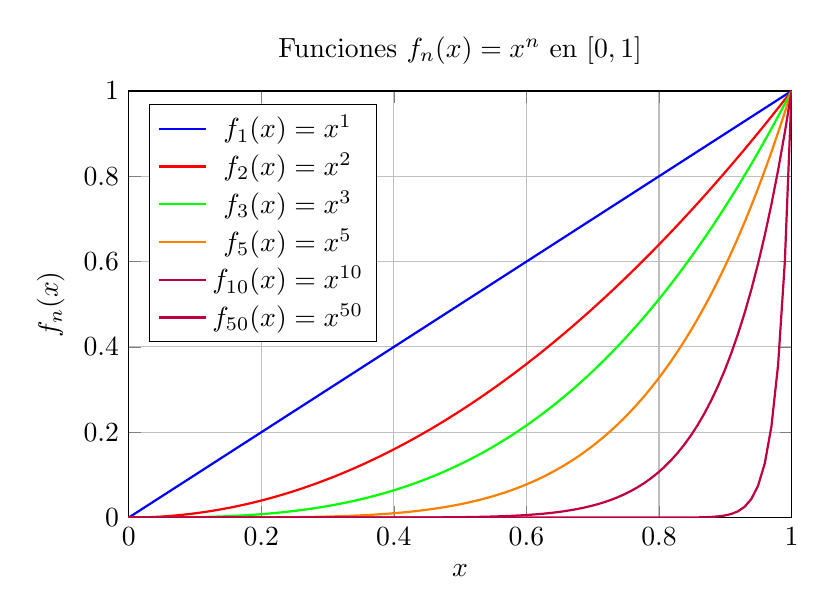
\begin{tikzpicture}
    \begin{axis}[
        width=10cm, height=7cm,
        xlabel={\(x\)},
        ylabel={\(f_n(x)\)},
        xmin=0, xmax=1,
        ymin=0, ymax=1,
        legend pos=north west,
        grid=major,
        title={Funciones \(f_n(x) = x^n\) en \([0, 1]\)}
      ]
      \addplot[domain=0:1, samples=100, thick, blue] {x^1};
      \addlegendentry{\(f_1(x) = x^1\)}

      \addplot[domain=0:1, samples=100, thick, red] {x^2};
      \addlegendentry{\(f_2(x) = x^2\)}

      \addplot[domain=0:1, samples=100, thick, green] {x^3};
      \addlegendentry{\(f_3(x) = x^3\)}

      \addplot[domain=0:1, samples=100, thick, orange] {x^5};
      \addlegendentry{\(f_5(x) = x^5\)}

      \addplot[domain=0:1, samples=100, thick, purple] {x^10};
      \addlegendentry{\(f_{10}(x) = x^{10} \)}

      \addplot[domain=0:1, samples=100, thick, purple] {x^50};
      \addlegendentry{\(f_{50}(x) = x^{50} \)}
    \end{axis}
  \end{tikzpicture}
\end{eg}

\begin{eg}
  \(f_n: [0, 2 \cdot \pi] \to \R \), \(f_n(x) = cos(nx)\) no converge puntualmente pues si \(x = \pi\), \(f_n(\pi) = (-1)^n\) y \(\nexists \lim_{n \to +\infty} f_n(\pi)\).
\end{eg}

Notemos que si \(f_n: X \subset \R \to \R \) converge puntualmente a \(f: X \to \R \Rightarrow (\forall \e > 0)(\exists n_0 \in \N) : |f_n(x) - f(x)| < \e \) \((\forall n > n_0)\), pero \(n_0\) depende de \(\e \) y de \(x\). Si \(\e \) está fijo puede ser que ningún \(n_0 \in \N \) sirva \(\forall x \in X\).

\begin{eg}
  Tomemos \(f_n: [0, 1] \to \R \) dada por \(f_n(x) = x^n\). Si: \begin{align*}
    \e = \frac{1}{2} & \Rightarrow (\forall n \in \N) \, \exists x \in [0\text{, }1) : |f_n(x) - f(x)| \geq \e = \frac{1}{2} \\
                     & \iff |x^n - 0| \geq \frac{1}{2}
  \end{align*}
  En efecto pues dado \(n \in \N \), \(\lim_{x \to 1} x^n = 1\).
\end{eg}

\begin{definition}[Convergencia uniforme]
  \((f_n)_{n \in \N} \) converge uniformemente a \(f: X \to \R \) si \((\forall \e > 0)(\forall x \in X)(\exists n_0 \in \N) : (\forall n > n_0)\) \(|f_n(x) - f(x)| < \e \). Notamos \(f_n \rightrightarrows f\).
\end{definition}

De la definición se desprende que \((f_n)_{n \in \N} \) converge uniformemente a \(f\) si y solo si \begin{align*}
  \lim_{n \to +\infty} \sup_{x \in X} |f_n(x) - f(x)| = 0
\end{align*}

\begin{eg}
  Por el ejemplo anterior \(f_n: [0, 1] \to \R \) dada por \(f_n(x) = x^n\) no converge uniformemente.
  Consideremos \(f_n: [0, 1 - \delta]\) con \(\delta \in (0, 1) \Rightarrow \) la convergencia a \(f(x) = 0\) es uniforme.
  En efecto, dado \(\e > 0\) quiero ver que
  \begin{align*}
    \exists n_0 \in \N : |x^n - 0| = x^n < \e \quad \forall n > n_0 \, \forall x \in [0, 1 - \delta].
  \end{align*}
  Como \(x^n\) es creciente entonces
  \begin{align*}
     & 0 \leq x^n \leq (1 - \delta)^n                                                                                      \\
     & \text{Como } \lim_{n \to +\infty} (1 - \delta)^n = 0                                                                \\
     & \Rightarrow \text{Dado } \e > 0 \quad \exists n_0 \in \N \, : \, |(1 - \delta)^n - 0 | < \e \quad \forall n > n_0   \\
     & \Rightarrow |x^n - 0| \leq |(1 - \delta)^n - 0| < \e \quad \forall n > n_0 \quad \forall x \in [0\text{, }1-\delta]
  \end{align*}
  \(\therefore \) la convergencia es uniforme.
\end{eg}

\begin{definition}[Sucesión de Cauchy]
  \((f_n)_{n \in \N} \), \(f_n: X \to \R \) es de Cauchy si \(\forall \e > 0\), \(\exists n_0 \in N : \forall n\),\(m > n_0\),\(\forall x \in X\), \(|f_n(x) - f_m(x)| < \e \).
\end{definition}

\begin{theorem}
  Una sucesión de funciones \(f_n : X \to \R \) es uniformemente convergente \(\iff \) es de Cauchy.
  \begin{proof}
    Para la ida tomemos \(\e > 0\), luego \(\exists n_0 \in \N : |f_n(x) - f(x)| < \frac{\e}{2} \) \((\forall n > n_0)(\forall x \in X)\) por hipótesis. Luego si \(n, m > n_0 \Rightarrow |f_n(x) - f_m(x)| < |f_n(x) - f(x)| + |f_m(x) - f(x)| < \e \) \((\forall x \in X)\). \\
    Para la vuelta tenemos que \(\forall x \in X\) \((f_n(x))_{n \in \N} \) es una sucesión de Cauchy que converge a un límite que llamo \(f(x)\). Dado \(\e > 0\), \(\exists n_0 \in \N : |f_n(x) - f_m(x)| < \e \) \((\forall n, m > n_0)\). \(\forall x \in X\) fijado el \(x\) y el \(n\) tomamos \(m \to +\infty \therefore |f_n(x) - f(x)| < \e \) \((\forall x \in X)(\forall n > n_0) \therefore \) la convergencia es uniforme.
  \end{proof}
\end{theorem}

\(f = \sum f_n\) es un caso particular del límite.
\(f : X \to \R \), \(f_n: X \to \R \). \(f = \lim_{n \to +\infty} S_n\), \(S_n\) la suma parcial, luego
\begin{align*}
  \sum f_n \rightrightarrows f \iff (\forall \e > 0) \, (\exists n_0 \in \N) \, : \, |S_{n+1}(x) - S_n(x)| < \e \quad (\forall n > n_0) \, (\forall x \in X)
\end{align*}

\begin{definition}[Convergencia normal]
  Decimos que \(\sum f_n: X \to \R \) converge normalmente si
  \begin{align*}
     & \exists (a_n)_{n \in \N} \subset \R : \sum a_n < +\infty \text{ y } \\
     & |f_n(x)| < a_n \quad (\forall n \in \N)(\forall x \in X).
  \end{align*}
\end{definition}

\begin{eg}
  \(\sum_{n \geq 1} \frac{sen(nx)}{n^2} \) es normalmente convergente pues \(|\frac{sen(nx)}{n^2}| \leq \frac{1}{n²} \) \((\forall n \in N)\) y \(\sum \frac{1}{n²} \) converge.
\end{eg}

\begin{theorem}[Test de Weierstrass]
  Si \(\sum f_n\) es normalmente convergente \(\Rightarrow \sum |f_n|\) y \(\sum f_n\) son uniformemente convergentes.
  \begin{proof}
    \(X\) el dominio de todas las \(f_i \Rightarrow (\forall n \in \N)(\forall p \in \N)(\forall x \in X) \Rightarrow \) \begin{align*}
      |S_{n + p}(x) - S_n(x)| & = |f_{n+1}(x) + \cdots + f_{n + p}(x)| \\
      & \leq |f_{n+1}(x)| + \cdots + |f_{n+p}(x)| \\
      & \leq a_{n+1} + \cdots + a_{n+p} < \e
    \end{align*}
    Por la hipótesis de la convergencia normal \(\therefore \sum f_n\) y \(\sum |f_n|\) convergen uniformemente.
  \end{proof}
\end{theorem}

Notemos que la convergencia normal implica la convergencia uniforme que a su vez implica la convergencia puntual, pero el camino inverso no vale.

\begin{eg}
  Sea \(f_n : [1\text{, }+\infty)\) dada por \begin{align*}
    f_n(x) = \begin{cases}
               \frac{1}{x} & \text{si } x \in [n, n+1], \\
               0           & \text{caso contrario.}
             \end{cases}
  \end{align*}
  Si llamamos \(f: [1\text{, } +\infty) \to \R \) a \(f(x) = \frac{1}{x} \).
  Afirmo que \(\sum_{n \geq 1} f_n \rightrightarrows f\). En efecto, pues
  \begin{align*}
     & 0 \leq f(x) - S_n < \frac{1}{n} \quad (\forall x \in [1\text{, } +\infty)) \text{ pues si }                                                                  \\
     & x \leq n+1 \Rightarrow f(x) = \frac{1}{x} \text{ y } S_n = \frac{1}{x} \text{ i.e } x \in [1\text{, } n+1) \Rightarrow \text{ la suma parcial no se anula, } \\
     & x > n+1 \Rightarrow f(x) = \frac{1}{x} \text{ y } S_n = 0 \text{ i.e no aparece en la suma.}
  \end{align*}
  Pero no converge normalmente en \([1, +\infty)\), pues si fuese \(f(x) \leq a_n\) \((\forall x \in [1, +\infty))\) tomando \(x = n \Rightarrow \frac{1}{n} \leq a_n \Rightarrow \sum a_n = +\infty\) y no puede ser normal la serie.
\end{eg}

\begin{note}
  Sea \((f_n)_{n \in \N} \) nos preguntamos si el límite en \(x\) y en \(n\) son intercambiables. La respuesta en general es no.
\end{note}

\begin{eg}
  \(f_n(x) = x^n\), \(f(x) = \begin{cases}
      1 & \text{si } x = 1,        \\
      0 & \text{si } 0 \leq x < 1.
    \end{cases} \) \begin{align*}
    & \lim_{x \to 1} \left(\lim_{n \to \infty} f_n(x)\right) = \lim_{x \to 1} f(x) = 0 \\
    & \lim_{n \to \infty} \left(\lim_{x \to 1} f_n(x)\right) = \lim_{n \to \infty} \left(\lim_{x \to 1} x^n\right) = \lim_{n \to \infty} 1 = 1
  \end{align*}
\end{eg}

\begin{theorem}
  Sea \(a\) un punto de acumulación de \(X\). Si la sucesión \(f_n: X \to \R \) converge uniformemente a \(f: X \to \R \) y \((\forall n \in \N)(\exists \lim_{x \to a} f_n(x) = L_n) \Rightarrow \)
  \begin{enumerate}
    \item \(\exists \lim_{n \to \infty} L_n\).
    \item \(L = \lim_{x \to a} f(x)\).
  \end{enumerate}
  Es decir que \begin{align*}
    \lim_{n \to \infty}\left(\lim_{x \to a} f_n(x)\right) = \lim_{x \to a}\left(\lim_{n \to \infty} f_n(x)\right)
  \end{align*}
  Siempre que los límites de adentro existan y el de la sucesión de funciones sea uniforme.

  \begin{proof}
    Para ver que \(\exists \lim_{n \to \infty} L_n = L\). Probemos que \(L_n\) es de Cauchy.
    \begin{enumerate}
      \item Dado \(\e > 0\), como \(f_n \rightrightarrows f\), entonces
            \begin{align*}
               & \exists n_0 \in \N : |f_n(x) - f_m(x)| < \frac{\e}{3}  \quad (\forall n > n_0)(\forall x \in X)                 \\
               & \text{Si } m, n > n_0, \exists x \in X : |L_m - f_m(x)| < \frac{\e}{3} \text{ y } |L_n - f_n(x)| < \frac{\e}{3} \\
               & \Rightarrow
              \begin{aligned}[t]
                |L_n - L_m| & \leq |L_n - f_n(x)| + |f_n(x) - f_m(x)| + |f_m(x) - L_m| \\
                            & < \frac{\e}{3} + \frac{\e}{3} + \frac{\e}{3} = \e
              \end{aligned}
            \end{align*}
      \item Veamos que si \(f(x) = \lim_{n \to \infty} f_n\) verifica \(\lim_{x \to a} f(x) = L\). Dado \(\e > 0\),
            \begin{align*}
               & \exists n_0 \in \N : |L_n - L| < \frac{\e}{3} \quad \forall n > n_0 \quad \forall x \in X                                                                       \\
               & \text{Si } n > n_0 \Rightarrow \exists \delta > 0 \, : \, 0 < |x-a| < \delta \Rightarrow |f_n(x) - L_n| < \frac{\e}{3} \text{ pues }\lim_{x \to a} f_n(x) = L_n \\
               & \Rightarrow \text{ Si } |x-a| < \delta \Rightarrow |f(x) - L| < \e
            \end{align*}
    \end{enumerate}
  \end{proof}
\end{theorem}

\begin{corollary}
  Sea \(a \in X\) punto de acumulación. Si \begin{enumerate}
    \item \(\sum f_n \rightrightarrows f\) en \(X\)
    \item \(\forall n \in \N \), \(\exists \lim_{x \to a} f_n(x) = L_n\)
  \end{enumerate} \(\Rightarrow \sum L_n < +\infty\) y \(\sum L_n = \lim_{x \to a} f(x)\).
  Es decir que \begin{align*}
    \lim_{x \to a}\left(\sum f_n(x)\right) = \sum\left(\lim_{x \to a} f_n(x)\right)
  \end{align*} Siempre que \(\sum f_n\) sea uniformemente convergente.
\end{corollary}

Notemos que el teorema también vale si \(a = +\infty\)
\begin{align*}
  \lim_{n \to +\infty} \left(\lim_{x \to +\infty} f_n(x)\right) = \lim_{x \to +\infty}\left(\lim_{n \to +\infty} f_n(x)\right)
\end{align*}
Siempre que los límites de adentro existan y la convergencia de la sucesión de funciones sea uniforme. La demostración queda como ejercicio.

\begin{theorem}
  Si \(f_n \rightrightarrows f\) y todas las \(f_n\) son continuas en \(a \in X \Rightarrow f\) es continua en \(a\).
  \begin{proof}
    Si \(a\) es punto aislado es inmediato. Si \(a \in X^{\prime} \Rightarrow \) \begin{align*}
      \lim_{x \to a} f(x) & = \lim_{x \to a}\left(\lim_{n \to \infty} f_n(x)\right)                                     \\
                          & = \lim_{n \to \infty}\left(\lim_{x \to a} f_n(x)\right) = \lim_{n \to \infty} f_n(a) = f(a)
    \end{align*}
  \end{proof}
\end{theorem}

Si el límite de \((f_n)_{n \in \N} \) no es continuo y las funciones de la sucesión sí, el límite no puede ser uniforme. Por otro lado que el límite sea continuo tampoco alcanza para que la convergencia sea uniforme.

\begin{definition}[Convergencia monótona]
  Decimos que \((f_n)_{n \in \N} \) converge monótonamente a \(f\), si \((\forall x \in X)\) la sucesión \((f_n)_{n \in \N} \) es monótona y \(f_n(x) \to f(x)\).
\end{definition}

\begin{theorem}
  Sea \(X \subset \R \) compacto. Si una sucesión de funciones continuas \(f_n: X \to \R \) converge monótonamente a una función continua \(f: X \to \R \Rightarrow \) la convergencia es uniforme.
  \begin{proof}
    Dado \(\e > 0\), definamos
    \begin{align*}
      K_n & = \{ x \in X : |f_n(x) - f(x)| \geq \e \} \quad (\forall n \in \N) \\
          & = |f_n(x) - f(x)|^{-1}([\e, +\infty))
    \end{align*}
    Como \(f_n\), \(f\) son continuas, \(K_n\) es cerrado de \(X \Rightarrow K_n\) es compacto \((\forall n \in \N)\). Afirmo que como \((f_n)\) es monótona,
    \(K_1 \supset K_2 \supset K_3 \supset \cdots \).
    En efecto, si \begin{enumerate}
      \item \(f_1 < f_2 < \cdots < f_n < \cdots < f \Rightarrow -f_1 > -f_2 \Rightarrow f - f_1 > |f - f_2| \Rightarrow K_1 \supset K_2 \cdots \).
      \item \(f_1 > f_2 > \cdots > f_n > \cdots < f \Rightarrow f_1 - f > |f - f_2| \Rightarrow K_1 \supset K_2 \cdots \).
    \end{enumerate}
    Pero además debe ser \(\bigcap_{n \in \N} K_n = \varnothing \) porque si no \(|f(x) - f_n(x)| \geq \e \) \((\forall n \in \N)\) absurdo
    \(\Rightarrow \exists n_0 \in \N : K_{n_0} = \varnothing \Rightarrow K_n = \varnothing \) \((\forall n > n_0) \Rightarrow |f(x) - f_n(x)| < \e \) \((\forall n > n_0)(\forall x \in X)\).
  \end{proof}
\end{theorem}

\begin{corollary}
  Una serie convergente de funciones no negativas, continuas, definidas en un compacto es uniformemente convergente \(\iff \sum f_n(x)\) es continua en un compacto.
  \begin{proof}
    \(S_n = f_1 + \cdots + f_n\) es una sucesión monótona pues son no negativas.
  \end{proof}
\end{corollary}

\section{Integración de sucesiones de funciones}

\begin{theorem}
  Si \(f_n: [a, b] \to \R \) son funciones integrables que convergen uniformemente a \(f: [a, b] \to \R \Rightarrow \) es integrable y vale que \(\int_a^b f(x) dx = \lim_{n \to +\infty} \int_a^b f_n(x) dx\).
  \begin{proof}
    Sean \(D_n\) y \(D\) los conjuntos de discontinuidad de \(f_n\) y \(f\). Si \(x \notin D_n\) \((\forall n \in \N) \Rightarrow x \notin D\),
    pues el límite uniforme es continuo en los puntos de discontinuidad.
    Luego \(D \subseteq \bigcup_{n \in \N} D_n\) Como \(|D_n| = 0\) \((\forall n \in \N)\), pues son integrables,
    tenemos que \(|D| = 0 \Rightarrow f\) es integrable. Ahora, dado \(\e > 0\),
    \(\exists n_0 \in \N : |f_n(x) - f(x)| < \frac{\e}{b-a} \) \((\forall x \in [a, b])(\forall n > n_0)\). Luego \((\forall n > n_0)\)
    \begin{align*}
      \left|\int_a^b f(x) dx - \int_a^b f_n(x) dx\right| \leq \int_a^b |f(x) - f_n(x)|dx < \frac{\e}{b-a} \cdot (b-a) = \e
    \end{align*}
    Es decir que \(\int_a^b \lim_{n \to +\infty} f_n(x) dx = \lim_{n \to +\infty} \int_a^b f_n(x) dx\).
  \end{proof}
\end{theorem}

\begin{corollary}
  Si \(\sum f_n \rightrightarrows f\) y las \(f_n\) son integrables \(\Rightarrow \) la suma es integrable y \(\int_a^b \sum f_n = \sum \int_a^b f_n\) en otras palabras, la serie se puede integrar término a término.
\end{corollary}

\begin{note}
  Si \(f_n: [a, b] \to \R \) son integrables y convergen puntualmente a \(f\) en \([a, b]\) puede pasar que \(f\) no sea integrable por ejemplo si \(\Q \cap [a, b] = \{r_1, \cdots \} \) y
  \begin{align*}
    f_n(x) = \begin{cases}
               1 & \text{si } x \in \{r_1, \ldots, r_n\}, \\
               0 & \text{caso contrario}.
             \end{cases}
  \end{align*}
  Luego \(f(x) = \begin{cases}
      1 & \text{si } x \in \Q \cap [a, b], \\
      0 & \text{caso contrario}.
    \end{cases} \Rightarrow f_n \to f \text{ en } [a, b]\), cada \(f_n\) es integrable, pero \(f\) no lo es.
\end{note}

\begin{note}
  \(f_n \to f\) en \([a, b]\), \(f_n\) y \(f\) son integrables, pero \(\lim_{n \to \infty} \int_a^b f_n \neq \int_a^b f\). Por ejemplo si \(f_n: [0, 1] \to \R \), \(f_n(x) = \begin{cases}
      (n+1) x^{n+1} & \text{si } x \in [0, 1), \\
      0             & \text{si } x = 1.
    \end{cases} \) Luego si \(f: [0, 1] \to \{0\} \), \(f(x) = 0 \Rightarrow f_n \to f\), pero \(\int_0^1 f_n(x) dx = 1 \neq 0 = \int_0^1 f(x) dx\).
\end{note}

\newpage\thispagestyle{empty}\blankpage

\chapter{Clase XXI - 15/11}
\section{Diferenciación de sucesiones de funciones}

\section{Series de potencia}

\section{Familias equicontinuas}

\newpage\thispagestyle{empty}\blankpage

\chapter{Clase XXII - 22/11}
  \section{Equicontinuidad uniforme}

  \begin{theorem}
  Si $E$ es una familia de funciones derivables en $I : \exists c > 0 : |f^{\prime}(x)| \leq c$ $(\forall f \in E)(\forall x \in I) \Rightarrow E$ es equicontinua en $I$.
  \begin{proof}
    Sea $x_0 \in I$, $\e > 0$, $\delta = \frac{\e}{c}$. Si $x \in I$ y $|x - x_0| < \delta \Rightarrow |f(x) - f(x_0)| \leq c |x - x_0| < c \cdot \frac{\e}{c} < \e$ $(\forall f \in E)$ usando Teorema del Valor Medio.
  \end{proof}
\end{theorem}

Más en general, con el mismo argumento, se ve que si $\forall x \in I$, $\exists c_x > 0$ y un intervalo $I_x$ tal que $x \in I_x \subset I$ y $|f^{\prime}(y)| \leq c_x$ $(\forall f \in E)(\forall y \in I_x) \Rightarrow E$ es equicontinua. 

\begin{definition}[Equicontinuidad uniforme]
  Una familia $E$ de funciones, $f: X \to \R$ se dice uniformemente equicontinua si $(\forall \e > 0)(\exists \delta > 0) : x, y \in X$, $|x-y| < \delta \Rightarrow |f(x) - f(y)| < \e$ $(\forall f \in E)$
\end{definition}

\begin{eg}
  $E$ es una familia de funciones derivables en $I$ y $|f^{\prime}(x)| \leq c$ $(\forall f \in E) \Rightarrow E$ es uniformemente equicontinua
\end{eg}

\begin{eg}
  Una familia formada por una única función continua, pero uniformemente continua es una familia equicontinua, pero no uniformemente.
\end{eg}

\begin{theorem}
  Sea $K \subset \R$ compacto. Toda familia de funciones $f: K \to \R$ equicontinua es uniformemente equicontinua.
  \begin{proof}
    Si $E$ no fuese uniformemente equicontinua, $\exists \e > 0 : (\forall n \in \N)$, $x_n$, $y_n \in K$, $f_n \in E : |x_n - y_n| < \frac{1}{n} < \delta$, pero $|f_n(x_n) - f_n(y_n)| \geq \e$. 
    Pasando a una subsucesión, podemos suponer que $x_n \to x \in K$ ($K$ es compacto) y como $|y_n - x_n| < \frac{1}{n}$ tenemos que $y_n \to x$. \\
    Como la familia $E$ es equicontinua en $x$, $\exists \delta > 0 : z \in K$ y $|x - z| < \delta \Rightarrow |f(x) - f(z)| < \frac{\e}{2}$ $(\forall f \in E) \Rightarrow |f_n(x_n) - f_n(y_n)| \leq |f_n(x_n) - f_n(x)| + |f_n(y_n) - f(x)| < \e$ $(\forall n > n_0 \in \N)$, pues $|x_n - x| < \delta$ y $|y_n - x| < \delta$ Absurdo! 
  \end{proof}
\end{theorem}

\begin{theorem}
  Si una sucesión equicontinua de funciones $f_n: X \to \R$ converge puntualmente en un subconjunto denso $D \subset X \Rightarrow f_n$ converge uniformemente sobre cualquier compacto $K \subset X$.

  \begin{proof}
    Sea $\e > 0$ quiero ver que $\exists n_0 \in \N : |f_m(x) - f_n(x)| < \e$ ($\forall m, n > n_0)(\forall x \in K)$. Luego $\forall d \in D$, $\exists n_d \in \N : |f_m(d) - f_n(d)| < \frac{\e}{3}$ $(\forall n, m > n_d)$. \\
    Por otro lado $\forall y \in K$, $\exists$ un intervalo abierto $I_y$ (centrado en $y$) tal que $|f_n(x) - f(z)| < \frac{e}{3}$ $(\forall x, z \in X \cap I_y)(\forall n \in \N)$. Como $K$ es compacto del cubrimiento $K \subset \bigcup_{y \in K} I_y$ podemos extraer un subcubrimiento finito $K \subset I_1 \cup I_2 \cup \cdots \cup I_p$. \\
    Como $D$ es denso en $X$, en cada intervalo $I_i$ podemos elegir $d_i \in D \cap I_i$. Sea $n_0 = max(n_{d_1}, \cdots n_{d_p}) \Rightarrow$ si $n, m > n_0$ y $x \in K \Rightarrow \exists i : x \in I_i$ así que \begin{equation}
      |f_m(x) - f_n(x)| \leq |f_m(x) - f_m(d_i)| + |f_m(d_i) - f_n(d_i)| + |f_n(d_i) - f_n(x)| < \e
    \end{equation} $\therefore$ es uniformemente equicontinua.
  \end{proof}
\end{theorem}

\begin{definition}[Acotada puntualmente]
  Una familia $E$ de funciones $f: X \to \R$, se dice puntualmente acotada si $\forall x \in X$, $\exists c_x > 0 : |f(x)| \leq c_x$ $(\forall f \in E)$.
\end{definition}

\begin{definition}[Uniformemente acotada]
  Se dice uniformemente acotada si $\exists c > 0 : |f(x)| < c$ $(\forall f \in E)(\forall x \in X)$.
\end{definition}

\begin{theorem}[Cantor - Tijonov]
  Sea $X \subset \R$ numerable. Toda sucesión puntualmente acotada de funciones $f: X \to \R$ posee una subsucesión puntualmente convergente.
  \begin{proof}
    Sea $X = \{x_1, \cdots\}$ como $(f_n)_{n \in \N}$ es acotada, tiene una subsucesión convergente $\Rightarrow \N_1 \subset \N$ infinito tal que $a_1 = \lim_{n \in \N_1} f_n(x_1)$. \\
    Como $(f_n(x_2))_{n \in \N_1}$ es acotada, $\exists \N_2 \subset \N_1$ infinito tal que $\exists a_2 = \lim_{n \in \N_2} f_n(x_2)$. Así siguiendo para cada $i \in \N$ tenemos $\N_1 \supset \N_2 \supset \cdots \supset \N_i \supset \cdots$, tales que $\lim_{n \in \N_i} f_n(x_i) = a_i$. \\
    Definimos a $\N^* \subset \N$ tomando como i-ésimo elemento de $\N^*$ al i-ésimo elemento de $\N_i \Rightarrow (\forall i \in \N) (f_n(x_i))_{n \in \N^*}$ es a partir del i-ésimo elemento una subsucesión de $(f_n(x_i))_{n \in \N_i}$ converge $\therefore$ Esto prueba que $(f_n)_{n \in \N^*}$ converge $\forall x_i \in X$.
  \end{proof}
\end{theorem}

\begin{theorem}[Arzelà - Ascoli]
  Sea $K \subset \R$ compacto, toda sucesión equicontinua y puntualmente acotada de funciones $f_n: K \to \R$ posee una subsucesión uniformemente convergente.
  \begin{proof}
    Como $K \subset \R$, $\exists X \subset K$ numerable y denso en $K$. Por el teorema anterior, como $X$ es numerable $(f_n)_{n \in \N}$ tiene una subsucesión puntualmente convergente en $X$ (por ser $f_n$ puntualmente acotada). Como $(f_n)_{n \in \N}$ es equicontinua y converge puntualmente en $X \subset K$ denso, converge uniformemente en $K$ por ser compacto. 
  \end{proof}
\end{theorem}

\section{Ecuaciones diferenciales}
TODO 

\newpage\thispagestyle{empty}\blankpage

\chapter{Parciales}
\section{Primer parcial - Primera fecha - 14/10}

\begin{enumerate}
  \item Dada $f: X \to Y$. Mostrar que $f$ es inyectiva $\iff f(A-B) = f(A) - f(B)$ para todo par de conjuntos $A, B \subseteq X$.
  \item Considerar $K$ un cuerpo ordenado y $f: K \to K$ definida por $f(x) = (1+x²)^{-1}$. Calcular, en el caso que existan: $inf(f(\Z))$ y $sup(f(\Z))$.
  \item Considerar $B \subseteq A$ conjuntos no vacíos de números reales. Se sabe que $A$ está acotado superior y que $\forall x \in A, \exists y \in B : x \leq y$. Demostrar que $sup A = sup B$.
  \item Demostrar, usando la definición que $\dfrac{4^n - 6}{4^{n+1}+10} \to \dfrac{1}{4}$.
  \item Decidir si las siguientes sucesiones son convergentes. En caso afirmativo, determinar su límite. \begin{enumerate}
    \item $a_1 = -\dfrac{3}{2}, 3 \cdot a_{n+1} = 2 + a_n^3$. Dar un valor de $a_1$ para que la sucesión converja a $-2$.
    \item $b_1 = 1, b_{n+1} = 1 + \dfrac{1}{b_n}$.
  \end{enumerate}
  \item Considerar una sucesión $(a_n)$ de términos positivos tal que $a_n \to L$. Demostrar que \begin{equation} \dfrac{n}{\dfrac{1}{a_1} + \dfrac{1}{a_2} + \cdots + \dfrac{1}{a_n}} \to L \end{equation} 
  \item Considerar $(a_n)$ y $(b_n)$ sucesiones acotadas superiormente mostrar que \begin{equation} \limsup(a_n + b_n) \leq \limsup a_n + \limsup b_n \end{equation} Dar un ejemplo donde la desigualdad sea estricta.
  \item Considerar $(a_n)$ sucesión de términos positivos tal que $\sum a_n$ es convergente. Decidir si la siguiente serie es convergente o divergente: $\sum \dfrac{\sqrt{a_n}}{n}$.
\end{enumerate}

\section{Primer parcial - Segunda fecha - 28/10}

\begin{enumerate}
  \item Considerar $(a_n)$ y $(b_n)$ tales que $a_n \to M$ y $b_n \to L \neq 0$. Demostrar usando la definición que $\dfrac{a_n}{b_n} \to \dfrac{M}{L}$.
  \item Considerar $f: X \to Y$ y $B \subset Y$. Demostrar que $f(f^{-1}(B)) \subseteq B$. Dar un ejemplo donde la desigualdad sea estricta.
  \item Decidir si la sucesión $b_{n+1} = \sqrt{2 + \sqrt{b_n}}$ con $b_1 = 1$ es convergente. En caso afirmativo, determinar su límite.
  \item Considerar $(x_n)$ la sucesión acotada tal que $\liminf x_n = \limsup x_n = L$. Demostrar que $x_n \to L$.
  \item Decidir si $\sum \dfrac{n! \cdot e^n}{n^{n+1}}$ es convergente o divergente.
  \item Considerar $(a_n)$ una sucesión decreciente tal que $\sum a_n$ es convergente. Demostrar que $n a_n \to 0$.
  \item Considerar $a_1 \geq a_2 \geq \cdots \geq 0$. Demostrar que $\sum a_n$ converge $\iff \sum 2^n \cdot a_{2^n}$ converge.
\end{enumerate}

\section{Segundo parcial - Primera fecha - 20/12}

\begin{enumerate}
  \item Sea $f : \R \to \R$ y $f_n(x) = f(nx), \forall n \in \N : (f_n)$ es equicontinua en $0$. Demostrar que $f$ es constante.
  \item Considerar $F$ cerrado y $K$ compacto en $\R^n$ tales que $F \cap K = \varnothing$. Demostrar que $d(F, K) > 0$. Se define $d(F, K) = inf\{ d(f, k) : f \in F, k \in K \}$. \\ Dar un ejemplo donde $F$ y $G$ sean cerrados disjuntos tales que $d(F, G) = 0$.
  \item Considerar $f: X \subseteq \R^n \to R$ una función tal que $\forall \e > 0, \exists g_{\e}: X \to \R$ continua tal que $\forall x \in X$ se cumple que $|f(x) - g_{\e}(x)| < \e$. Mostrar que $f$ es continua.
  \item \begin{enumerate}
    \item Considerar $f_n: X \to Y$ tales que $f_n \rightrightarrows f$ y $g: Y \to Z$ uniformemente continua. Demostrar que $g \circ f_n \rightrightarrows g \circ f$.
    \item Considerar $g_n : Y \to Z$ tales que $g_n \rightrightarrows g$ y $f: X \to Y$. Es cierto que $g_n \circ f \rightrightarrows g \circ f$?
  \end{enumerate}
  \item \begin{enumerate}
    \item Demostrar que $x^n(1-x)$ converge uniformemente a $0$ en $[0, 1]$.
    \item Estudiar la convergencia puntual y uniforme de las siguientes series en el intervalo $[0, 1]$. \begin{enumerate} \item $\sum_{n \geq 1} x^n(1-x)$ \item $\sum_{n \geq 1} (-1)^n x^n(1-x) $ \end{enumerate}
  \end{enumerate}
\end{enumerate}


\blankpage

\bibliographystyle{unsrt}
\bibliography{references}
\nocite{*}

\end{document}
